\chapter{An electronic analog of the Burridge-Knopoff model}
\label{chap: electronic analog of bk}

\section{Mechanical Burridge-Knopoff model}
\label{sec: mechanical bk}

The Burridge-Knopoff (BK) spring-block model \cite{ref:bk} is a two-dimensional system of massive blocks
lying on a rough horizontal surface. Each block is connected to its nearest neighbors by a set of springs,
and linked through another spring to an upper horizontal ceiling moving with constant velocity with respect to the lower plate,
as shown in Fig. \ref{fig bk}.

\begin{figure}[H]
    \centering
    \subfloat{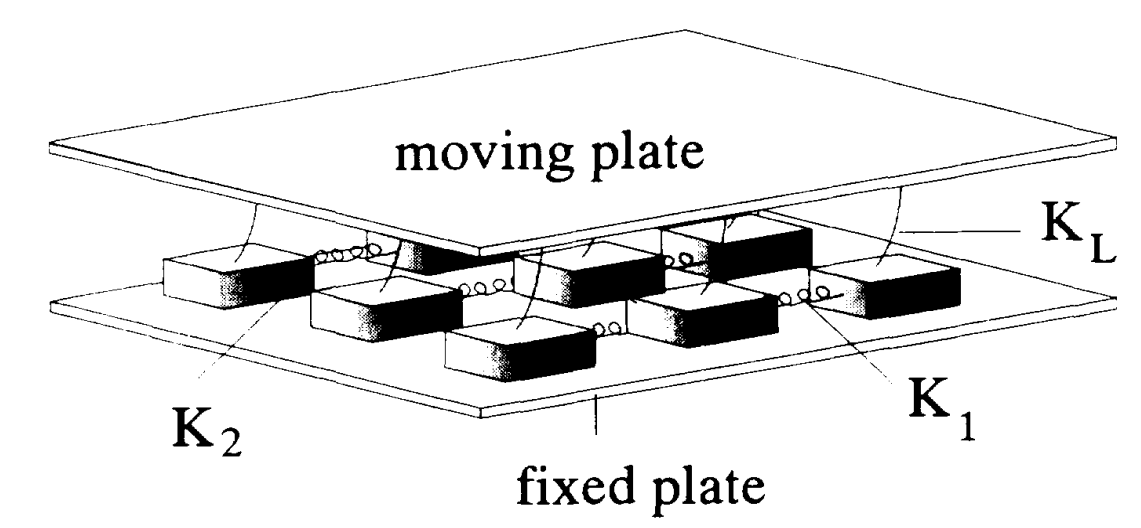
\includegraphics[width=0.42\linewidth]{images/BK1.png}}\\[0.43cm]
    \subfloat{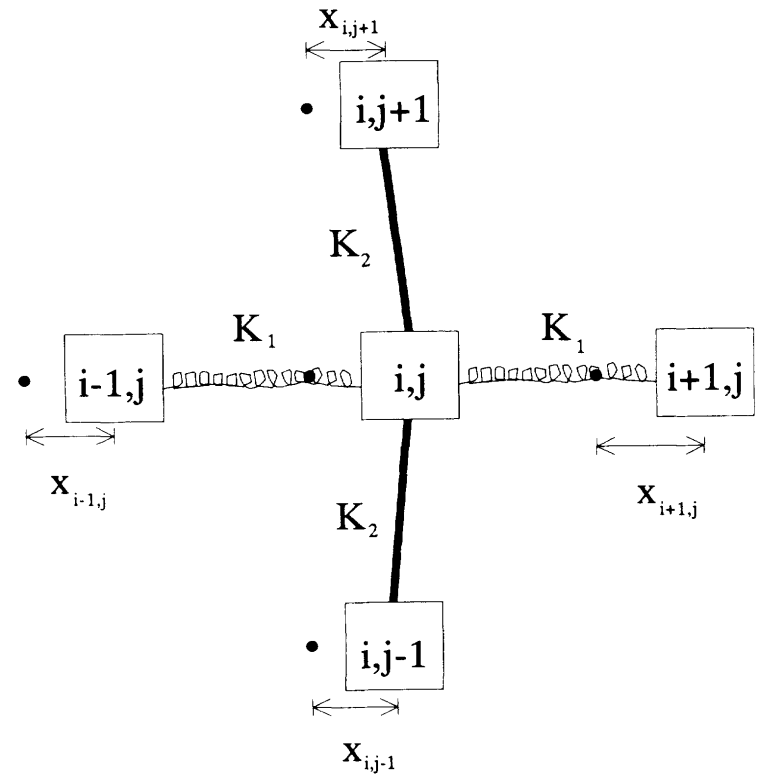
\includegraphics[width=0.42\linewidth]{images/BK2.png}}
    \caption{Visual representation of the Burridge-Knopoff spring-block model. $K_1$ and $K_2$
    are the elastic constants, respectively, of the horizontal and vertical springs, while $K_L$
    is the elastic constant of the springs connecting the blocks and the moving plate.
    The figure below represents the interaction between a block and its four nearest neighbors,
    as a function of the displacement $x_{i,j}$. Figure adapted from Ref. \cite{ref:ofc}.}
    \label{fig bk}
\end{figure}

The blocks are driven by the relative movement of the two rigid plates. When the force on one block
reaches some threshold value $F_{\text{th}}$, the block slips, and it is reasonable to assume that the
force on that block becomes zero. Then, the force on the four nearest neighbors is increased, often
resulting in further slips, and an avalanche can occur.

The purpose of the BK model is the description of the dynamical behavior of
real faults, whereby a constant, slow driving motion of plates produces an accumulation of ``stress''
up to a threshold at which such stress is released through an abrupt motion $-$ i.e., an earthquake $-$
of one or more of the system's constituent parts.

\subsection{Motion of two coupled blocks}
\label{subsec: diff eqs for two blocks}

The mechanical BK model for the motion of two coupled blocks is shown schematically in
Fig. \ref{fig: 2 blocks motion}. The upper ceiling moves with respect to the surface with
a constant velocity $u_d$. Let $x_1$, $x_2$ be the displacements of the block positions
relative to a state in which the springs are relaxed, and $u_1$, $u_2$ the velocities of the blocks in the
lower surface frame, so that $u_i=u_d+\dot{x}_i$ with $i=1,2$.

\begin{figure}[H]
    \centering
    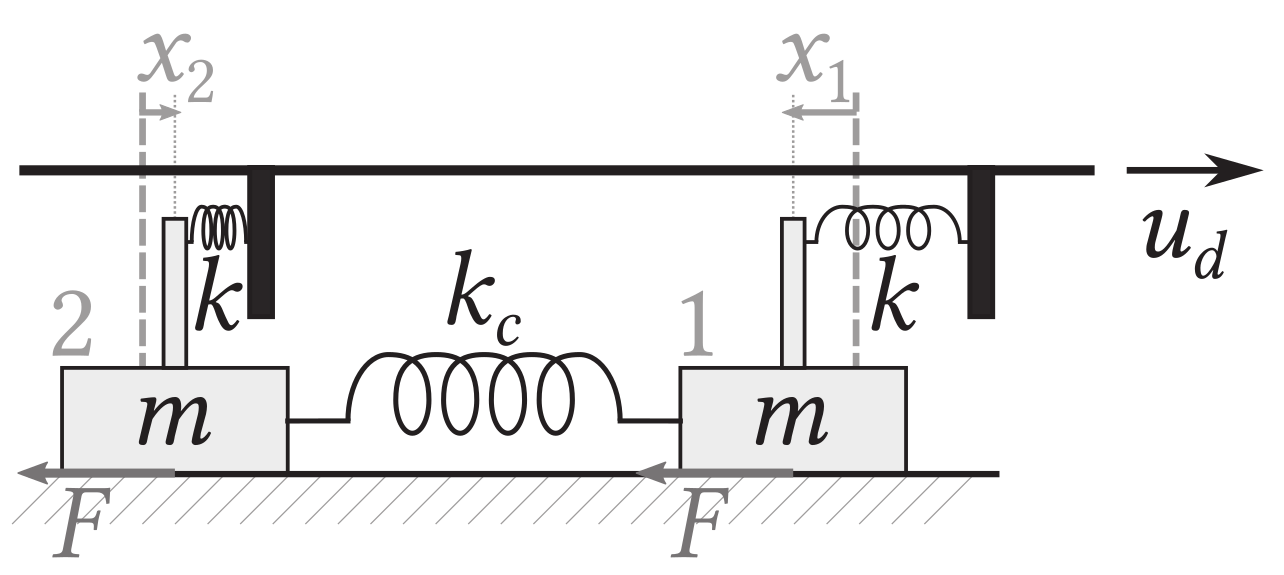
\includegraphics[width=0.5\linewidth]{images/bk_2_blocks.png}
    \caption{Two-blocks mechanical BK model. The upper ceiling, which the blocks
    are coupled to via springs with elastic constant $k$, is dragged with constant
    velocity $u_d$ with respect to the underlying surface. This surface exerts a nonlinear,
    velocity-dependent friction $F$ to each block's motion. Figure adapted from Ref. \cite{ref:electronic_analog}.}
    \label{fig: 2 blocks motion}
\end{figure}

The equations of motion are thus given by

\begin{equation}
\label{eq: 2 block motion}
    \begin{gathered}
    m\frac{\text{d}u_1}{\text{d}t} = -kx_1 - k_c(x_1-x_2) - F(u_1),\\[10pt]
    \frac{\text{d}x_1}{\text{d}t} = u_1 - u_d,\\[10pt]
    m\frac{\text{d}u_2}{\text{d}t} = -kx_2 - k_c(x_2-x_1) - F(u_2),\\[10pt]
    \frac{\text{d}x_2}{\text{d}t} = u_2 - u_d,
\end{gathered}
\end{equation}

where $m$ is the mass of the blocks, $k$ is the elastic constant of the springs that connect the blocks
to the ceiling, $k_c$ is the elastic constant of the spring linking the two blocks, and $F(u)$ is the nonlinear
velocity-dependent friction. The velocities are assumed to be non-negative.

\subsection{Dimensionless system}
\label{subsec: dimensionless 2 block motion}

It is possible to render this system dimensionless by defining the following dimensionless quantities ($i$ takes the values 1 and 2):
a time $\tau\equiv t\sqrt{k/m}$, a velocity $\nu_i\equiv u_i/u_0$, a position $\xi_i\equiv x_i \sqrt{k/m}/u_0$,
a friction $\varphi(\nu_i)\equiv F(\nu_i)/(u_0\sqrt{mk})$ and a parameter $\lambda\equiv k_c/k$.
The four equations of motion can then be written as

\begin{equation}
\label{eq: 2 block motion dimensionless}
\begin{gathered}
    \frac{\text{d}\nu_i}{\text{d}\tau}=-(1+\lambda)\xi_i+\lambda\xi_{3-i}-\varphi(\nu_i),\\[10pt]
    \frac{\text{d}\xi_i}{\text{d}\tau}=\nu_i-\nu_d.
\end{gathered}
\end{equation}

There exists a relative freedom in the choice of the friction $\varphi(\nu)$, provided that
(i) $\varphi(\nu<0)=0$, (ii) $\varphi(\nu\geq0)\geq0$ and (iii) $\varphi(\nu)$ decreases down to zero from a
maximum value $\varphi(0)$ that occurs at $\nu=0$.

It is useful to define the equations of motion also in the case of a lower surface moving with a positive
dimensionless velocity $\Delta\nu$, so that $\nu'_i=\nu_i+\Delta\nu$ and $\nu'_d=\nu_d+\Delta\nu$.
The system of equations becomes:

\begin{equation}
    \label{eq: 2 block motion dimensionless moving surface}
    \begin{gathered}
        \frac{\text{d}\nu'_i}{\text{d}\tau}=-(1+\lambda)\xi_i+\lambda\xi_{3-i}-\varphi(\nu'_i-\Delta\nu),\\[10pt]
        \frac{\text{d}\xi_i}{\text{d}\tau}=\nu'_i-\nu'_d.
    \end{gathered}
\end{equation}


\section{Electronic analog for the motion of two blocks}
\label{sec: electronic analog}

In order to analyze the properties of the BK model, it is possible to build an electronic circuit
which differential equations are the same as Eqs. \ref{eq: 2 block motion dimensionless moving surface}.
The first implementation was done by Field, Venturi and Nori \cite{ref:fvn} by drawing a direct parallelism
between mechanical and electrical quantities. The idea was to use capacitance as mass,
inductance as the reciprocal of elastic constant, voltage as velocity and current as position.
However, this implementation has two main drawbacks. The first one is the usage of inductances, which are typically
bulky and have intrinsically large tolerances compared with other components, resulting in higher uncertainties; moreover,
their tunability is very low. The second issue is that the current is a state variable, and it is less straightforward
to measure it with respect to voltage.

It is possible to use another implementation \cite{ref:electronic_analog} which does not rely on inductances
and uses only voltages as state variables. In order to do so it is necessary to rewrite the system equations
as integral equations, so that they can be implemented by electronic integrators that are more stable than
the differentiators. The new state variables are defined as $V_i\equiv \nu_i V_0$ and $W_i\equiv \xi_i V_0$ and
the new time constant is given by $\tau=RC$, where $R$ and $C$ are suitably chosen resistance and capacitance.
Integrating the system of Eqs. \ref{eq: 2 block motion dimensionless moving surface} for a moving surface and replacing
$V'_i\equiv V_i+\Delta V$ and $V'_d\equiv V_d+\Delta V$, where $V_d\equiv V_0\nu_d$ and $\Delta V\equiv V_0\Delta\nu$,
leads to the following system of equations:

\begin{equation}
    \label{eq: 2 block motion electronic}
    \begin{gathered}
        V_i+\Delta V=-\frac{1}{RC}\int\left[ (1+\lambda)W_i - \lambda W_{3-i}+V_0\varphi\left(\frac{V_i}{V_0}\right) \right]\text{d}t ,\\[10pt]
        W_i=-\frac{1}{RC}\int(V_d-V_i)\,\text{d}t,
    \end{gathered}
\end{equation}

where $\lambda=R/R_c$ and $R_c$ is a suitably chosen resistance.

These differential equations are implemented by the circuit shown in Fig. \ref{fig: circuit diagram},
which makes use of resistors, capacitors, diodes and operational amplifiers, without any inductance.
Assuming for a while that $\Delta V$ and the nonlinear element $\varphi(V_i/V_0)$ were not present,
the two integrations above could be promptly implemented by considering the black part of the circuit diagram.

\begin{figure}[H]
    \centering
    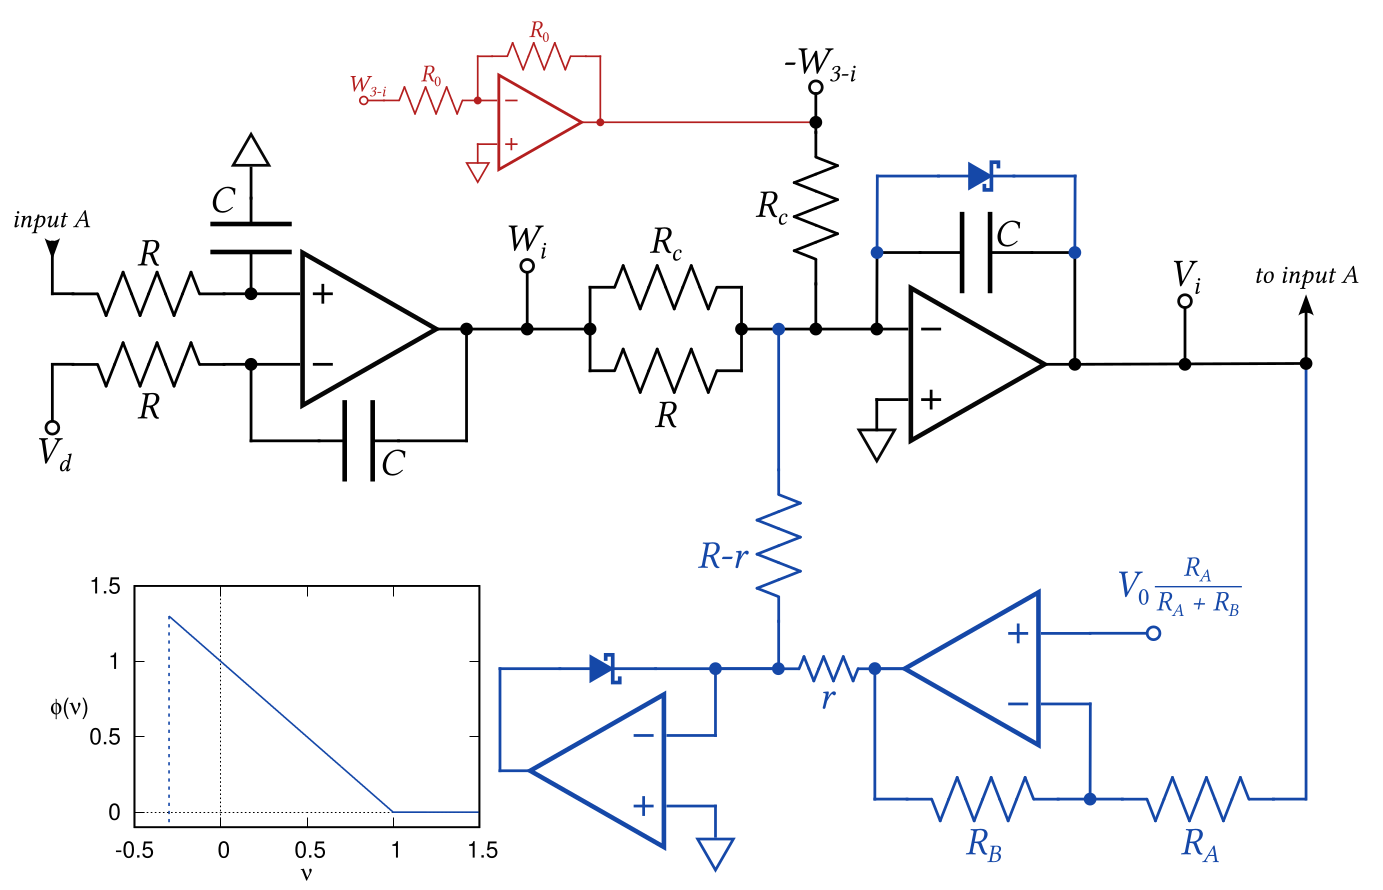
\includegraphics[width=\linewidth]
    {../1_block/breadboard/breadboard_implementation.png}
    \caption{Inductorless representation of the BK model. The circuit diagram refers to a single block, labeled by $i=1,2$.
    The bottom left plot shows the characteristic of the nonlinear element, i.e. the blue part of the diagram.
    The red part is a standard inverting operational amplifier, which is necessary for the coupling between two blocks.
    Figure adapted from Ref. \cite{ref:electronic_analog}.}
    \label{fig: circuit diagram}
\end{figure}

The nonlinear term is instead represented by the blue part of the diagram and it is implemented as follows.
A Schottky diode is inserted on the feedback network on the integrator producing $V_i$; this ensures that $V_i$ does not
drop below $-V_{\text{diode}}$, where $V_{\text{diode}}\approx 0.3$ V. In order to not contradict the constraint
that the ``velocity'' must be always non-negative, it is necessary to set $\Delta V = V_{\text{diode}}$.
In this way the first of the constraints set in Sec. \ref{subsec: dimensionless 2 block motion}, i.e. $\varphi(V_i < 0 )=0$
is satisfied, since the voltage cannot drop below zero.

The nonlinear friction element consists in a linear drop for the analog of the velocity-weakening force, and it is
implemented using two additional op-amps as follows. The output of the first op-amp is given by $V_0-V_iR_B/R_A$.
Downstream of the resistor $r$, this voltage is prevented to drop below zero by an active
clamp made of the second op-amp which has a diode in its feedback network. The resulting voltage is fed back into
the integrator generating $V_i$ through an additional resistor $R-r$.


\section{Characterization of the single block behavior}
\label{sec: single block characterization}

With the aim of analyzing the circuit represented in Fig. \ref{fig: circuit diagram},
it is necessary to characterize its behavior. The first characterization concerns the
function of a single block, in the absence of couplings.
In this case $\lambda=0$ and the differential equations of the system can be simplified as
(the subscript $i$ is omitted):

\begin{equation}
\label{eq: single block eq motion}
\begin{gathered}
    \frac{\text{d}^2V}{\text{d}t^2}+
    \frac{1}{\tau}\varphi'\left(\frac{V}{V_0}\right)\frac{\text{d}V}{\text{d}t}+
    \frac{1}{\tau^2}(V-V_d)=0\\[10pt]
    \frac{\text{d}W}{\text{d}t}=\frac{1}{\tau}(V-V_d)
\end{gathered}
\end{equation}

where $\varphi'$ is the derivative of the friction with respect to the velocity $V$.
The equation for the velocity is of the kind met in the classical description of stick-slip
vibrations \cite{ref:stick_slip}, i.e. of the self-sustained oscillations induced by friction.
This means that an oscillating behavior for $V$ and $W$ has to be expected.

In order to check the validity of these equations, the circuit was physically implemented
in two different manners. The first implementation was done on a breadboard using large
electronic components; the main issue with this system is that it is not scalable,
due to the fact that a single circuit occupies half of the entire space on the breadboard.
The second one consists instead in an integrated board in which 25 circuits
like the one in Fig. \ref{fig: circuit diagram} were implemented;
the scalability issue is solved in this case, so that this board could be utilized
to study the behavior of many coupled blocks, as will be done in the next chapters.

\subsection{Breadboard implementation}
\label{subsec:breadboard implementation}

The breadboard implementation was made using 1N5817 Schottky diodes
and OP27 op-amps; these op-amps were
supplied with $V_{CC}=\pm12~\text{V}$. The nominal values for the
resistances and capacitors are $R=R_c=10~\text{k}\Omega$,
$R_A=R_B=10~\text{k}\Omega$, $r=1.8~\text{k}\Omega$ and
$C=100~\text{nF}$, so that the characteristic time of the circuit is $\tau=1$ ms.
The input voltages are $V_0=1~\text{V}$ and
the variable voltage $V_d$, while the output voltages are
$V$ and $W$ (the subscript $i$ is omitted).

The single block behavior of this circuit is shown in Fig. \ref{fig:oscillation breadboard}.
As expected by Eqs. \ref{eq: single block eq motion}, both the velocity $V$ and the position $W$
exhibit an oscillating behavior. While $W$ closely resembles a sinusoidal wave, $V$ possesses
a lower clamping that makes it different from a simple wave; this clamping is due
to the presence of the Schottky diodes, which prevent that the velocity becomes negative, as
discussed in Sec. \ref{sec: electronic analog}.
In the end, both the frequency and the amplitude of the waves depend on the driving voltage $V_d$.

\begin{figure}
    \centering
    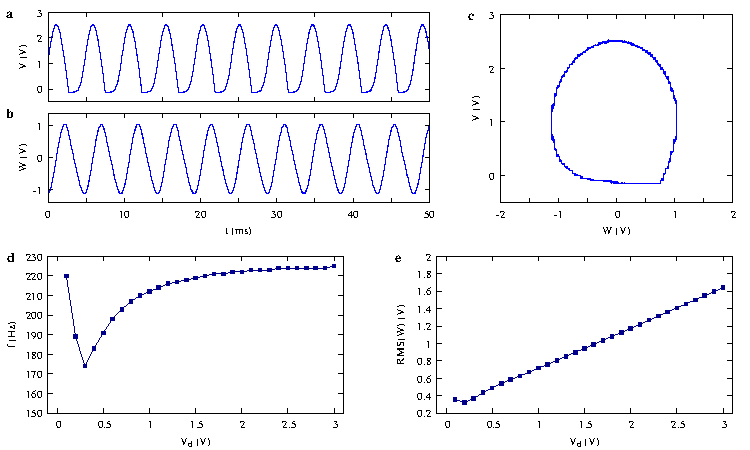
\includegraphics[width=\linewidth]{../1_block/breadboard/single_block.pdf}
    \caption{Oscillating behavior for the circuit implemented on
    the breadboard. (a) Plot of $W$ and (b) of $V$ as a function of time,
    for $V_d=1$ V.
    (c) Phase portrait (Lissajous figure) of $V$ versus $W$. (d)
    Frequency and (e) root mean square amplitude of the
    output signal $W$ as a function of the parameter $V_d$.}
    \label{fig:oscillation breadboard}
\end{figure}

%The lower clamping in the Lissajous
%figure is intended and is due to the presence of the Schottky diodes.
%The frequency behavior at high voltages,
%namely $V_d \gtrsim 1$ V, is the same for each kind of op-amp.
%On the other hand, the amplitudes possess an offset which depends on
%the selected op-amp; nonetheless, they all exhibit a mostly linear
%behavior.

\subsection{Integrated board implementation}
\label{subsec:integrated board implementation}

The circuit diagram for each of the 25 chips on the integrated board is equivalent to the
one shown in Fig. \ref{fig: circuit diagram}. The only differences with the breadboard implementation
concern the nonlinear components, i.e. the use of DFLS1100 Schottky diodes and quad operational
amplifiers OP470, which should offer comparable performances to the components used in the previous section,
i.e. 1N5817 Schottky diodes and OP27 op-amps.

A comparison between the single block behavior of this circuit and the one implemented in the previous section
is shown in Fig. \ref{fig:oscillation board}. The most notable difference is the amplitude of the waveforms and of
the Lissajous figures, which is higher in the integrated board case. Another discrepancy between the two plots lies
in the frequency behavior at low driving voltage $V_d$, i.e. the initial ``drop'' in the frequency is more pronounced
in the breadboard case with respect to the integrated circuit. These distinctions are all probably due to the different diodes
and op-amps utilized in the two cases, but they do not modify the actual dynamics of the circuit.

Despite being slightly different, both implementations comply with the oscillating behavior predicted by
Eqs. \ref{eq: single block eq motion}. It is thus reasonable to assume that both the integrated circuit and the one on the
breadboard can potentially be a consistent physical implementation of the BK model. In order to furtherly strenghten
this hypothesis, an analysis on the behavior of two coupled blocks will be carried out in the next section.
From now on, only the integrated board implementation will be considered, due to the scalability issues that were discussed
beforehand.

\begin{figure}
    \centering
    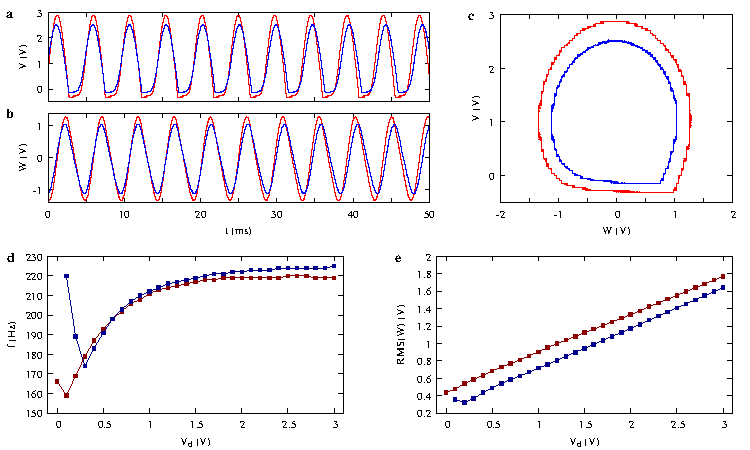
\includegraphics[width=\linewidth]{../1_block/board_new/single_block.pdf}
    \caption{Oscillating behavior for the circuit implemented on
    the integrated board (red) and the one implemented on the breadboard (blue).
    (a) Plot of $W$ and (b) of $V$ as a function of time, for $V_d=1$ V.
    (c) Phase portrait (Lissajous figure) of $V$ versus $W$. (d)
    Frequency and (e) root mean square amplitude of the
    output signal $W$ as a function of the parameter $V_d$.}
    \label{fig:oscillation board}
\end{figure}


\section{Characterization of the double block behavior}
\label{sec: double block characterization}

The coupling between two blocks is performed by connecting the inverted voltage $-W_2$ of the second block to the
inverting input of the op-amp generating $V_1$ on the first block (see Fig. \ref{fig: circuit diagram}), and viceversa, in order
to comply with Eqs. \ref{eq: 2 block motion electronic}.

The behavior of the two coupled blocks is shown in Fig. \ref{fig:2 blocks waveforms}.
By looking at the waveforms $V_i(t)$ and $W_i(t)$ it is possible to notice that the simple periodic behavior
is no longer observed. Furthermore, the Lissajous figures do not show a stationary orbit like the single block case.
This hints that the dynamics in the presence of coupling might be chaotic, i.e. deterministic but unpredictable,
and surely non-periodic.

Another way to check the presence of chaos in the system is to make use of a bifurcation diagram, i.e. the distribution
of the local maxima of a state variable (position, velocity) as a function of an external parameter (driving force).
This diagram is shown in Fig. \ref{fig: bifurcation} for the position $W_1$ ($W_2$ behaves similarly) as a function of $V_d$.
The scan of the $V_d$ parameter was carried out by switching off the circuit's power supply, changing the voltage $V_d$,
and the switching the power supply back on. This ensured that the recorded evolution was independent of the previous state.
It is possible to notice that the dynamics is richer for $V_d\lesssim0.1$ V, where several maxima can be detected.
In contrast, for $V_d\gtrsim0.1$ V, only one maximum can be observed; in this regime the system behaves similarly
to the single block case, manifesting periodic sinusoidal-like oscillations.

\begin{figure}
    \centering
    \begin{minipage}{.49\textwidth}
        \begin{subfigure}{\linewidth}
            \centering
            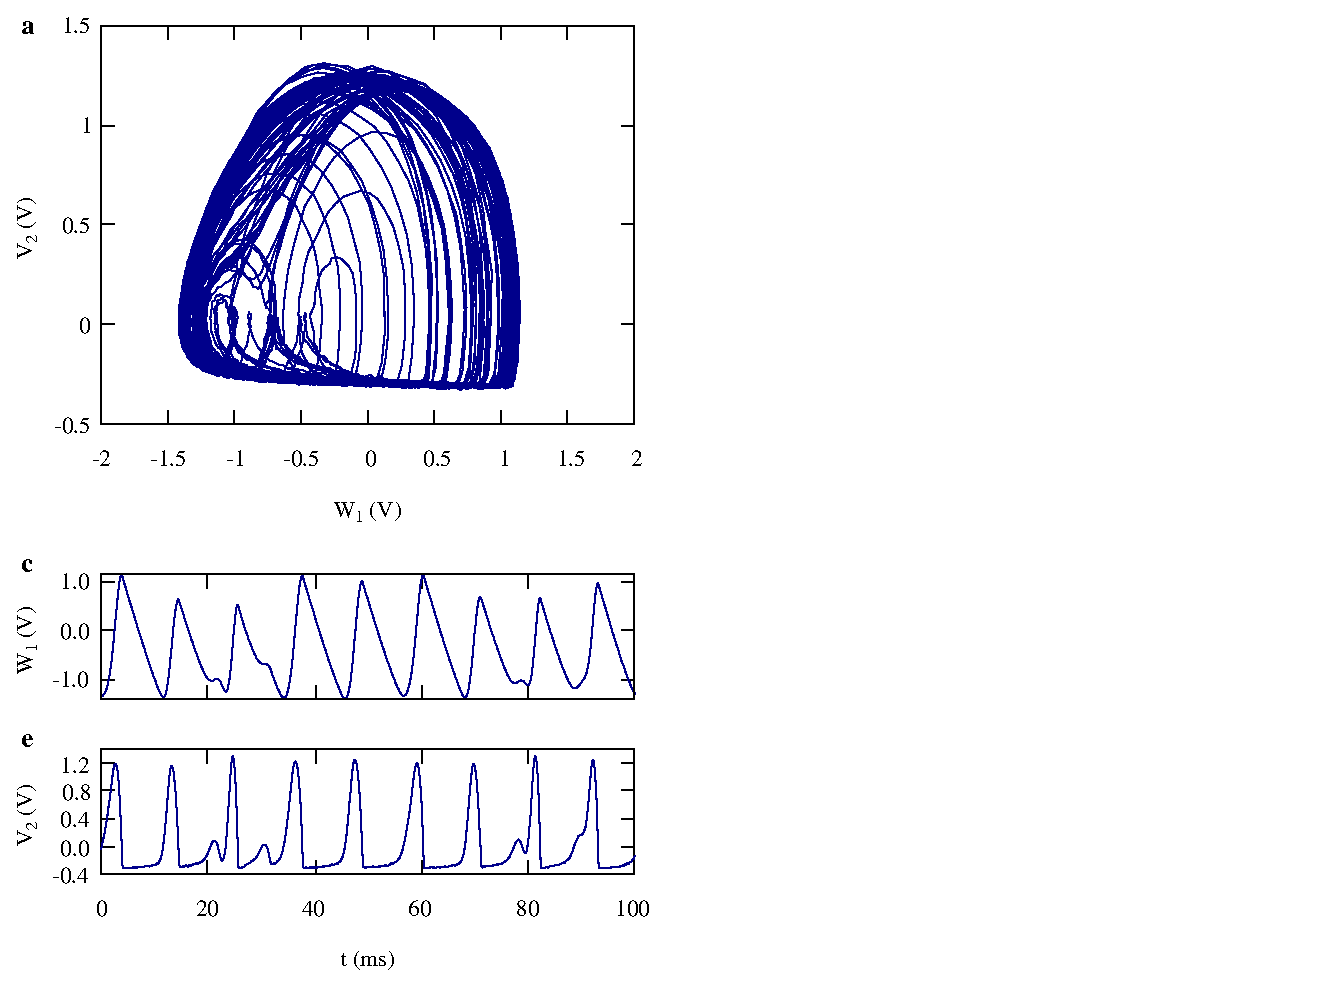
\includegraphics[width=\linewidth,trim={0cm 0 11cm 0},clip,center]
            {../2_blocks/4e4_points/plots/waveforms_1.pdf}
        \end{subfigure}
    \end{minipage}
    \begin{minipage}{.49\textwidth}
        \begin{subfigure}{\linewidth}
            \centering
            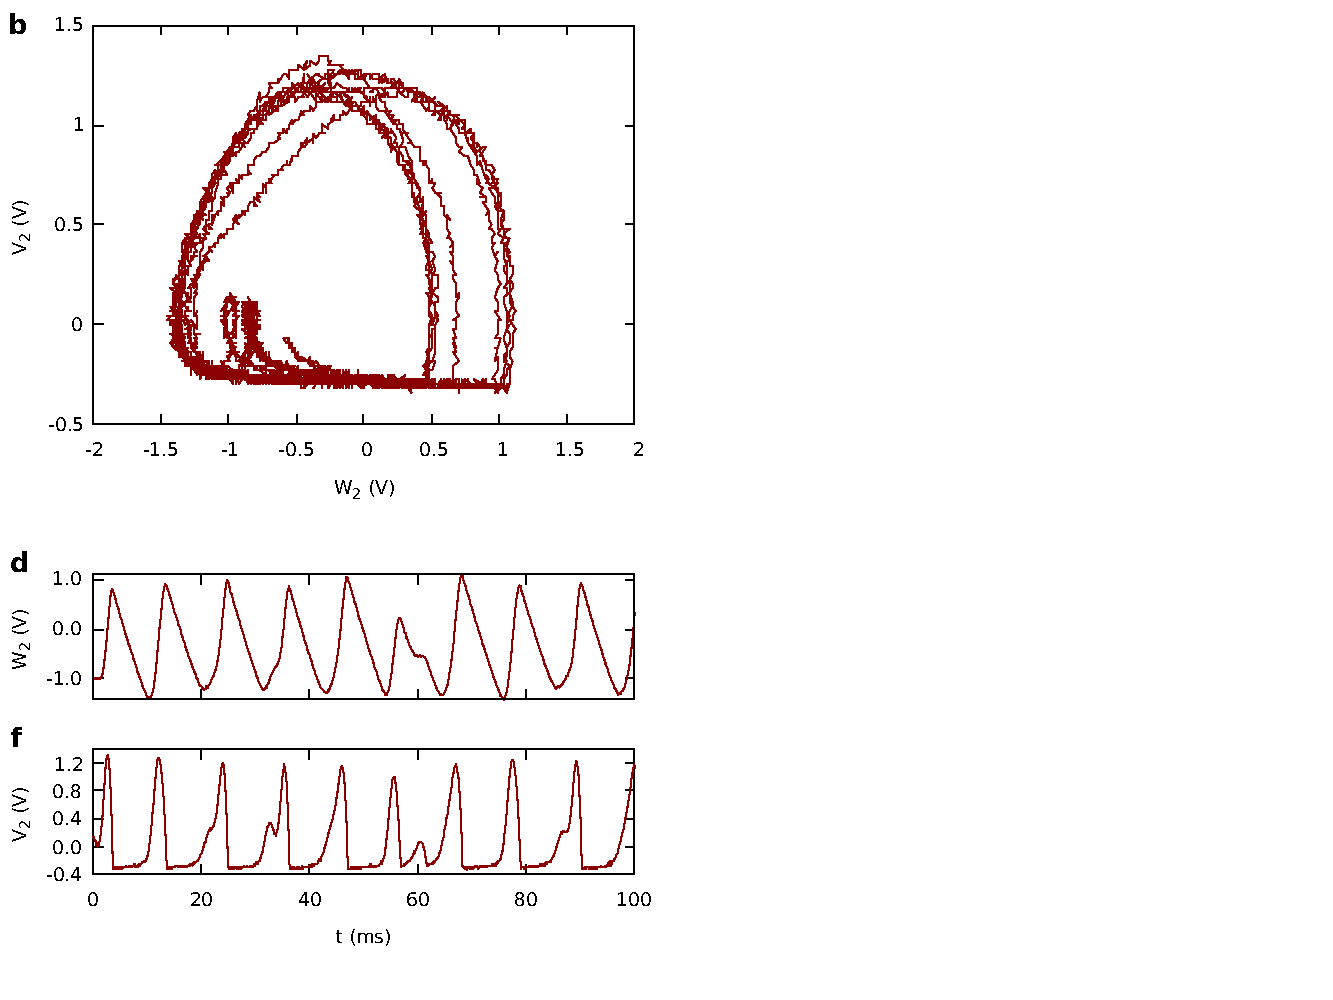
\includegraphics[width=\linewidth,trim={0cm 0 11cm 0},clip,center]
            {../2_blocks/4e4_points/plots/waveforms_2.pdf}
        \end{subfigure}
    \end{minipage}
    \caption{Chaotic behavior of two coupled blocks for $V_d=0.05$ V.
    Phase portraits of $V_i$ vs $W_i$ for the first (a) and second (b) block, for a total time of 1 s.
    Time series plots for $W_1$ (c), $V_1$ (e), $W_2$ (d) and $V_2$ (f), for a total time of 100 ms.}
    \label{fig:2 blocks waveforms}
\end{figure}

\begin{figure}[H]
    \centering
    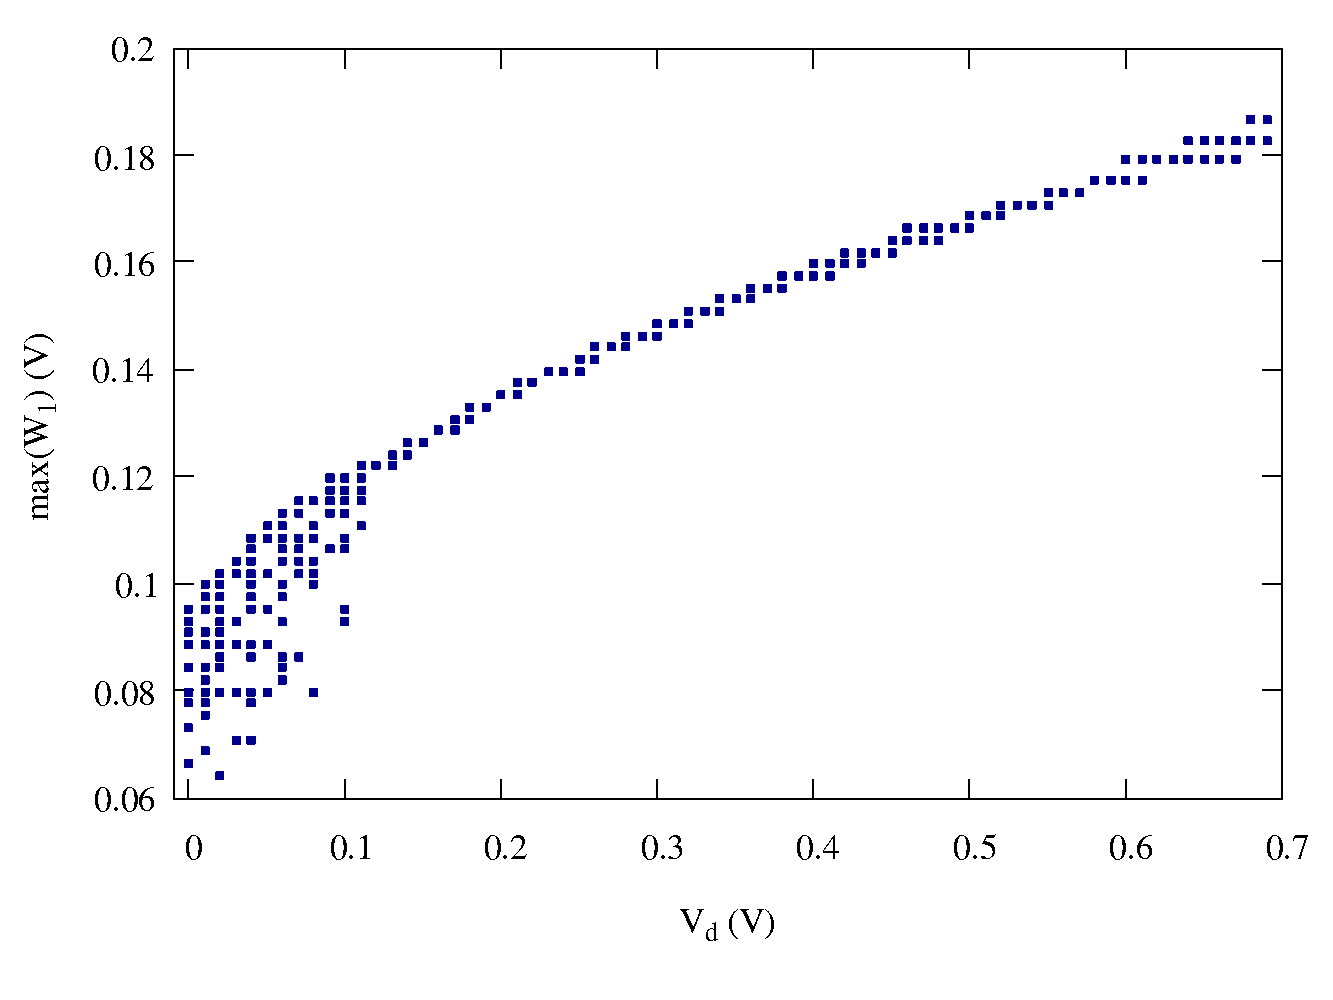
\includegraphics[width=0.6\linewidth]{../2_blocks/bifurcation/bifurcation.pdf}
    \caption{Bifurcation diagram for two coupled blocks.
    The local maxima of $W_1$ are plotted as a function of the external parameter $V_d$,
    which is varied in steps of 10 mV.}
    \label{fig: bifurcation}
\end{figure}

It is therefore safe to assume that, for low driving voltages $V_d$, the coupled system of two blocks shows a chaotic behavior.
The reason why this does not occur at higher voltages might be that the driving force is so strong that the blocks
behave independently of it. Nonetheless, these analyses are not enough to say that this circuit is actually a chaotic system.
In order to prove this statement, a deeper chaos analysis is carried out in the next chapter.





\begin{comment}

\section{Prototypes}\label{sec:prototypes}

In order to describe the coupling between many oscillators it is
not possible use the breadboard implementation of the circuit
shown in Fig. \ref{fig: circuit diagram}, due to
scalability issues. For the purpose of improving the system
scalability, two smaller prototypical chips have been built.
The circuit implemented in each chip is shown in Fig.
\ref{fig:prototype implementation}. The differences between this
circuit and the one used in the previous section lie in the nonlinear
elements; in this case MBRA210L Schottky diodes have been used,
as well as quad operational amplifiers OP470, which offer
comparable performance to OP27 op-amps.

The oscillating behavior of this circuit is shown in Fig.
\ref{fig:oscillation prototype} for both chips. These systems are much
less stable with respect to the circuit implemented on the breadboard;
in fact, measurements were possible only in a small range for $V_d$,
namely $V_d \leq 1.1$ V for one chip and $V_d \leq 0.6$ V for the
other one. It is also important to point out that the diode clamping
is not present; in fact, it is only noticeable at voltages
$V_d \lesssim 0.4$ V.


\begin{figure}[H]
    \centering
    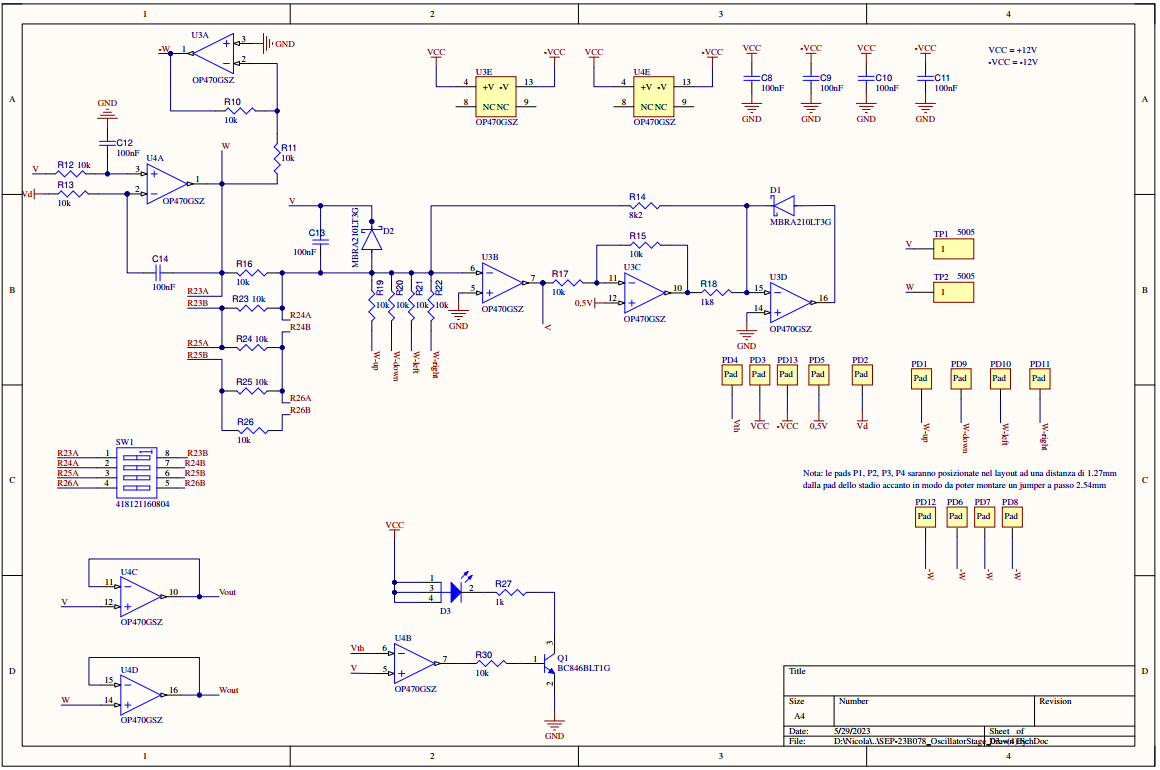
\includegraphics[width=0.75\linewidth]
    {../1_block/prototypes/prototype_implementation.png}
    \caption{Circuit diagram of one prototypical chip.}
    \label{fig:prototype implementation}
\end{figure}

\begin{figure}[H]
    \centering
    \begin{minipage}{.58\textwidth}
        \begin{subfigure}{\linewidth}
            \centering
            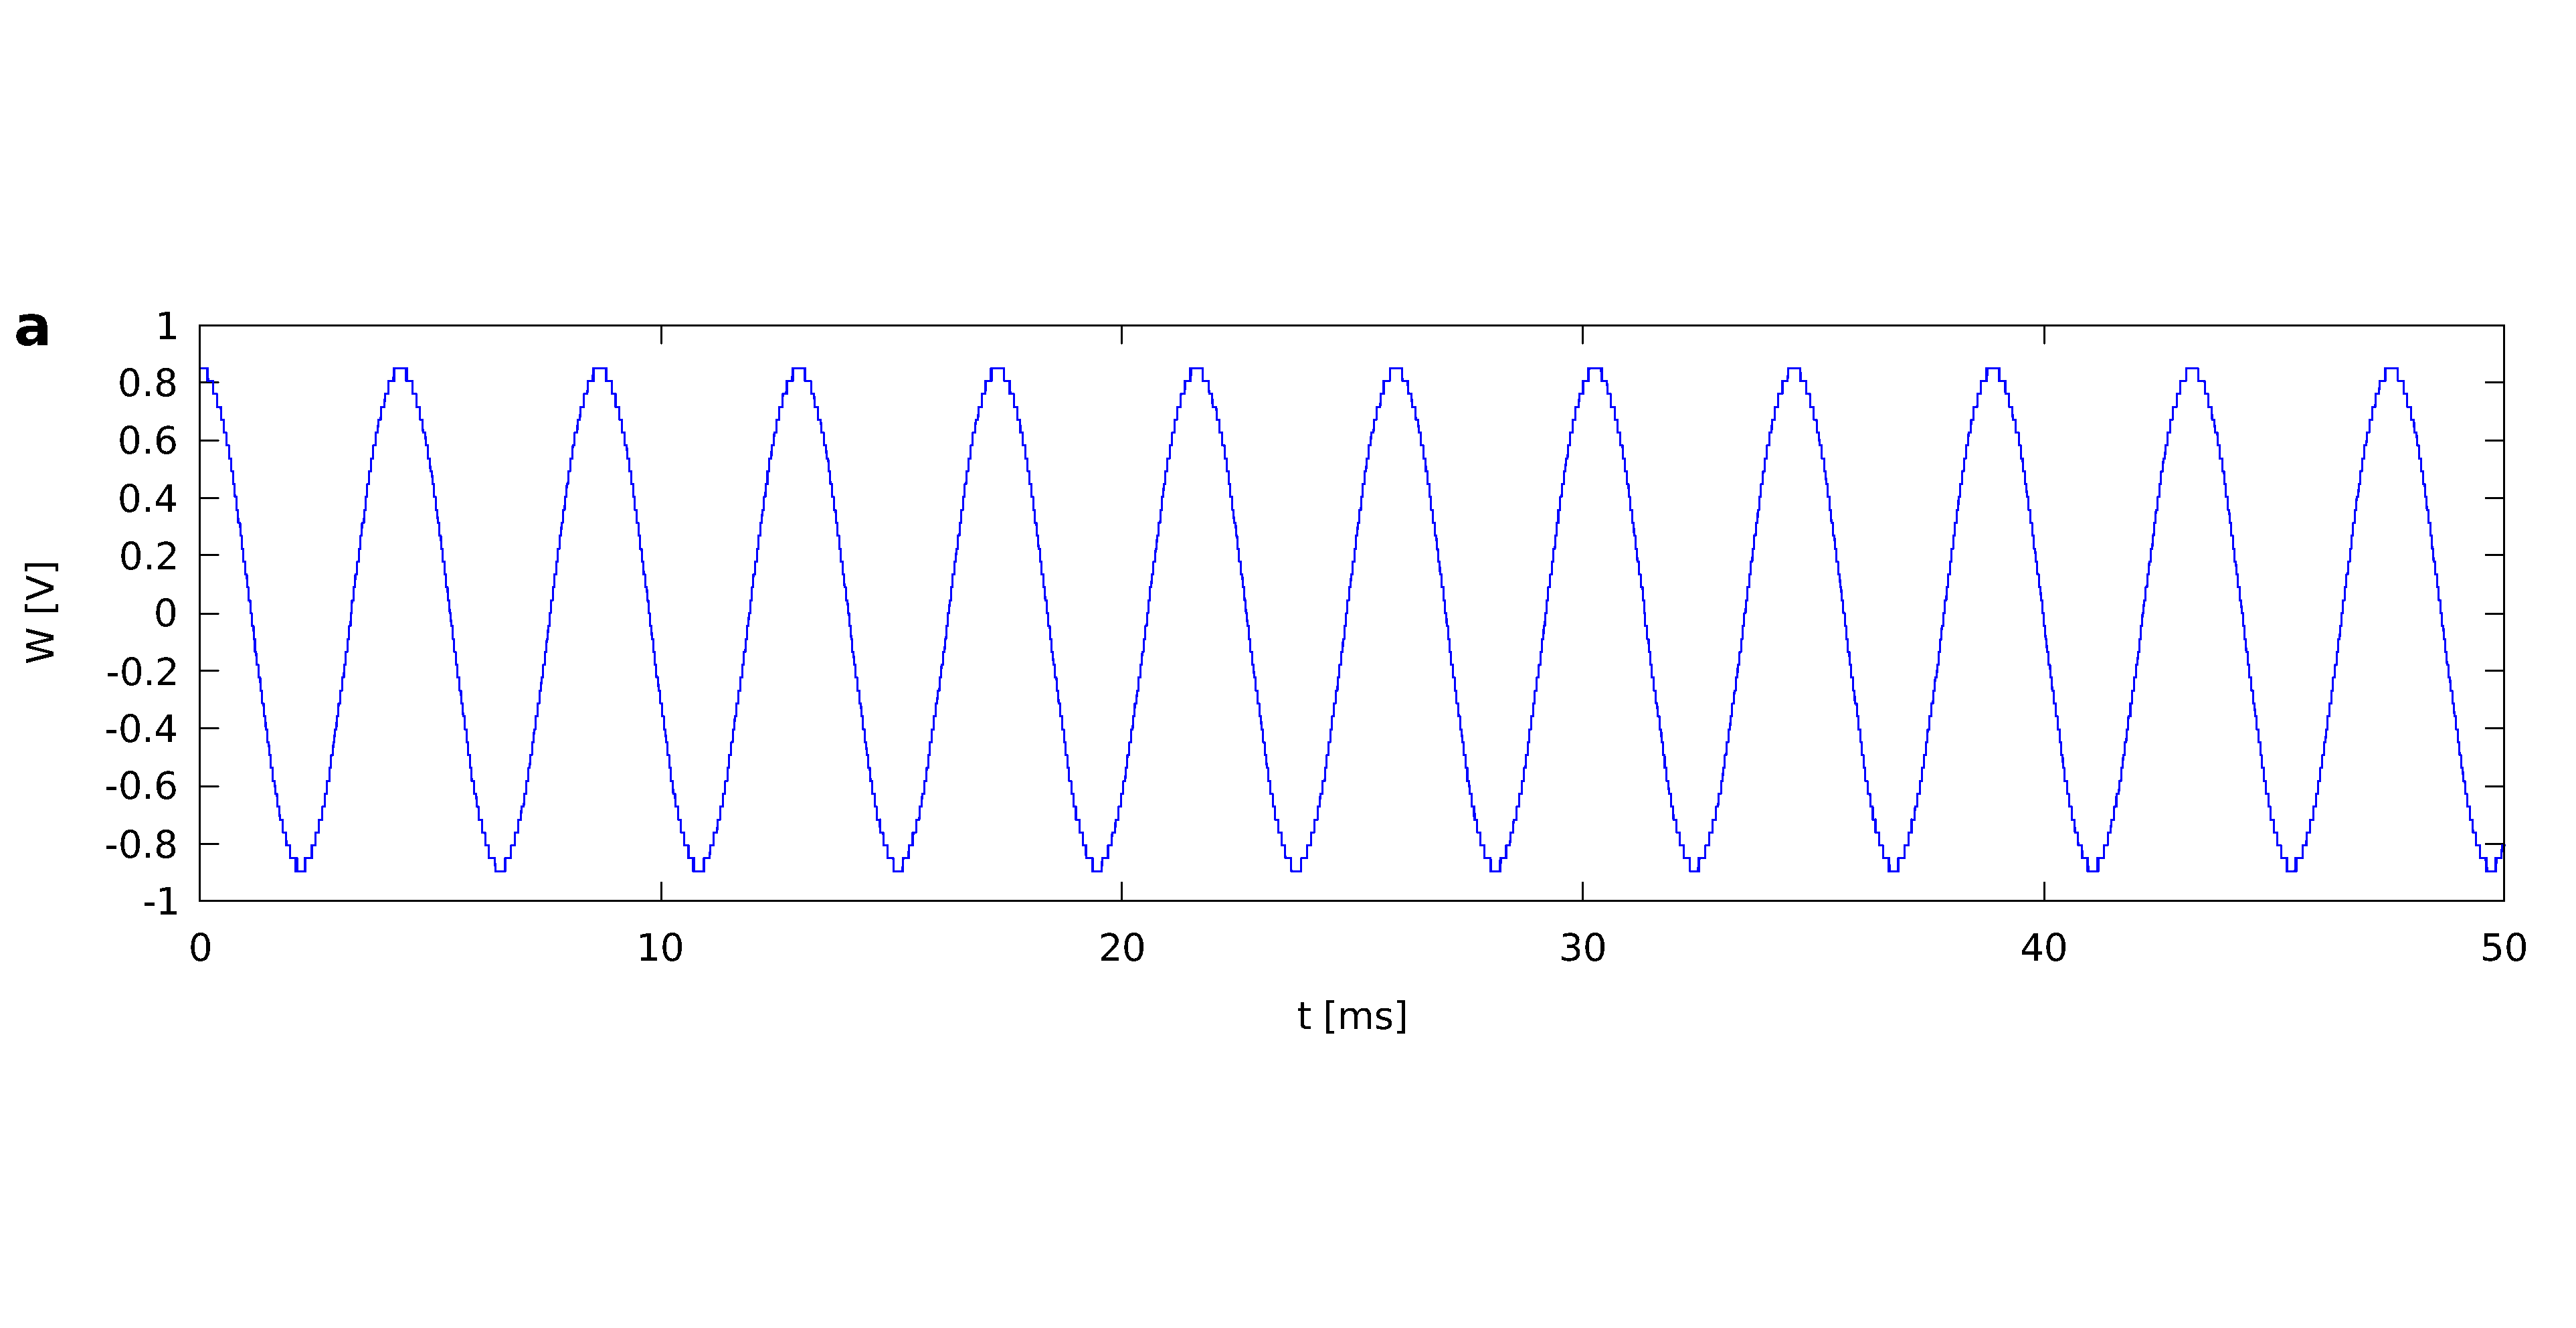
\includegraphics[width=\linewidth,trim={0 6cm 0 6cm},clip,left]
            {../1_block/prototypes/W_wf.pdf}\\
            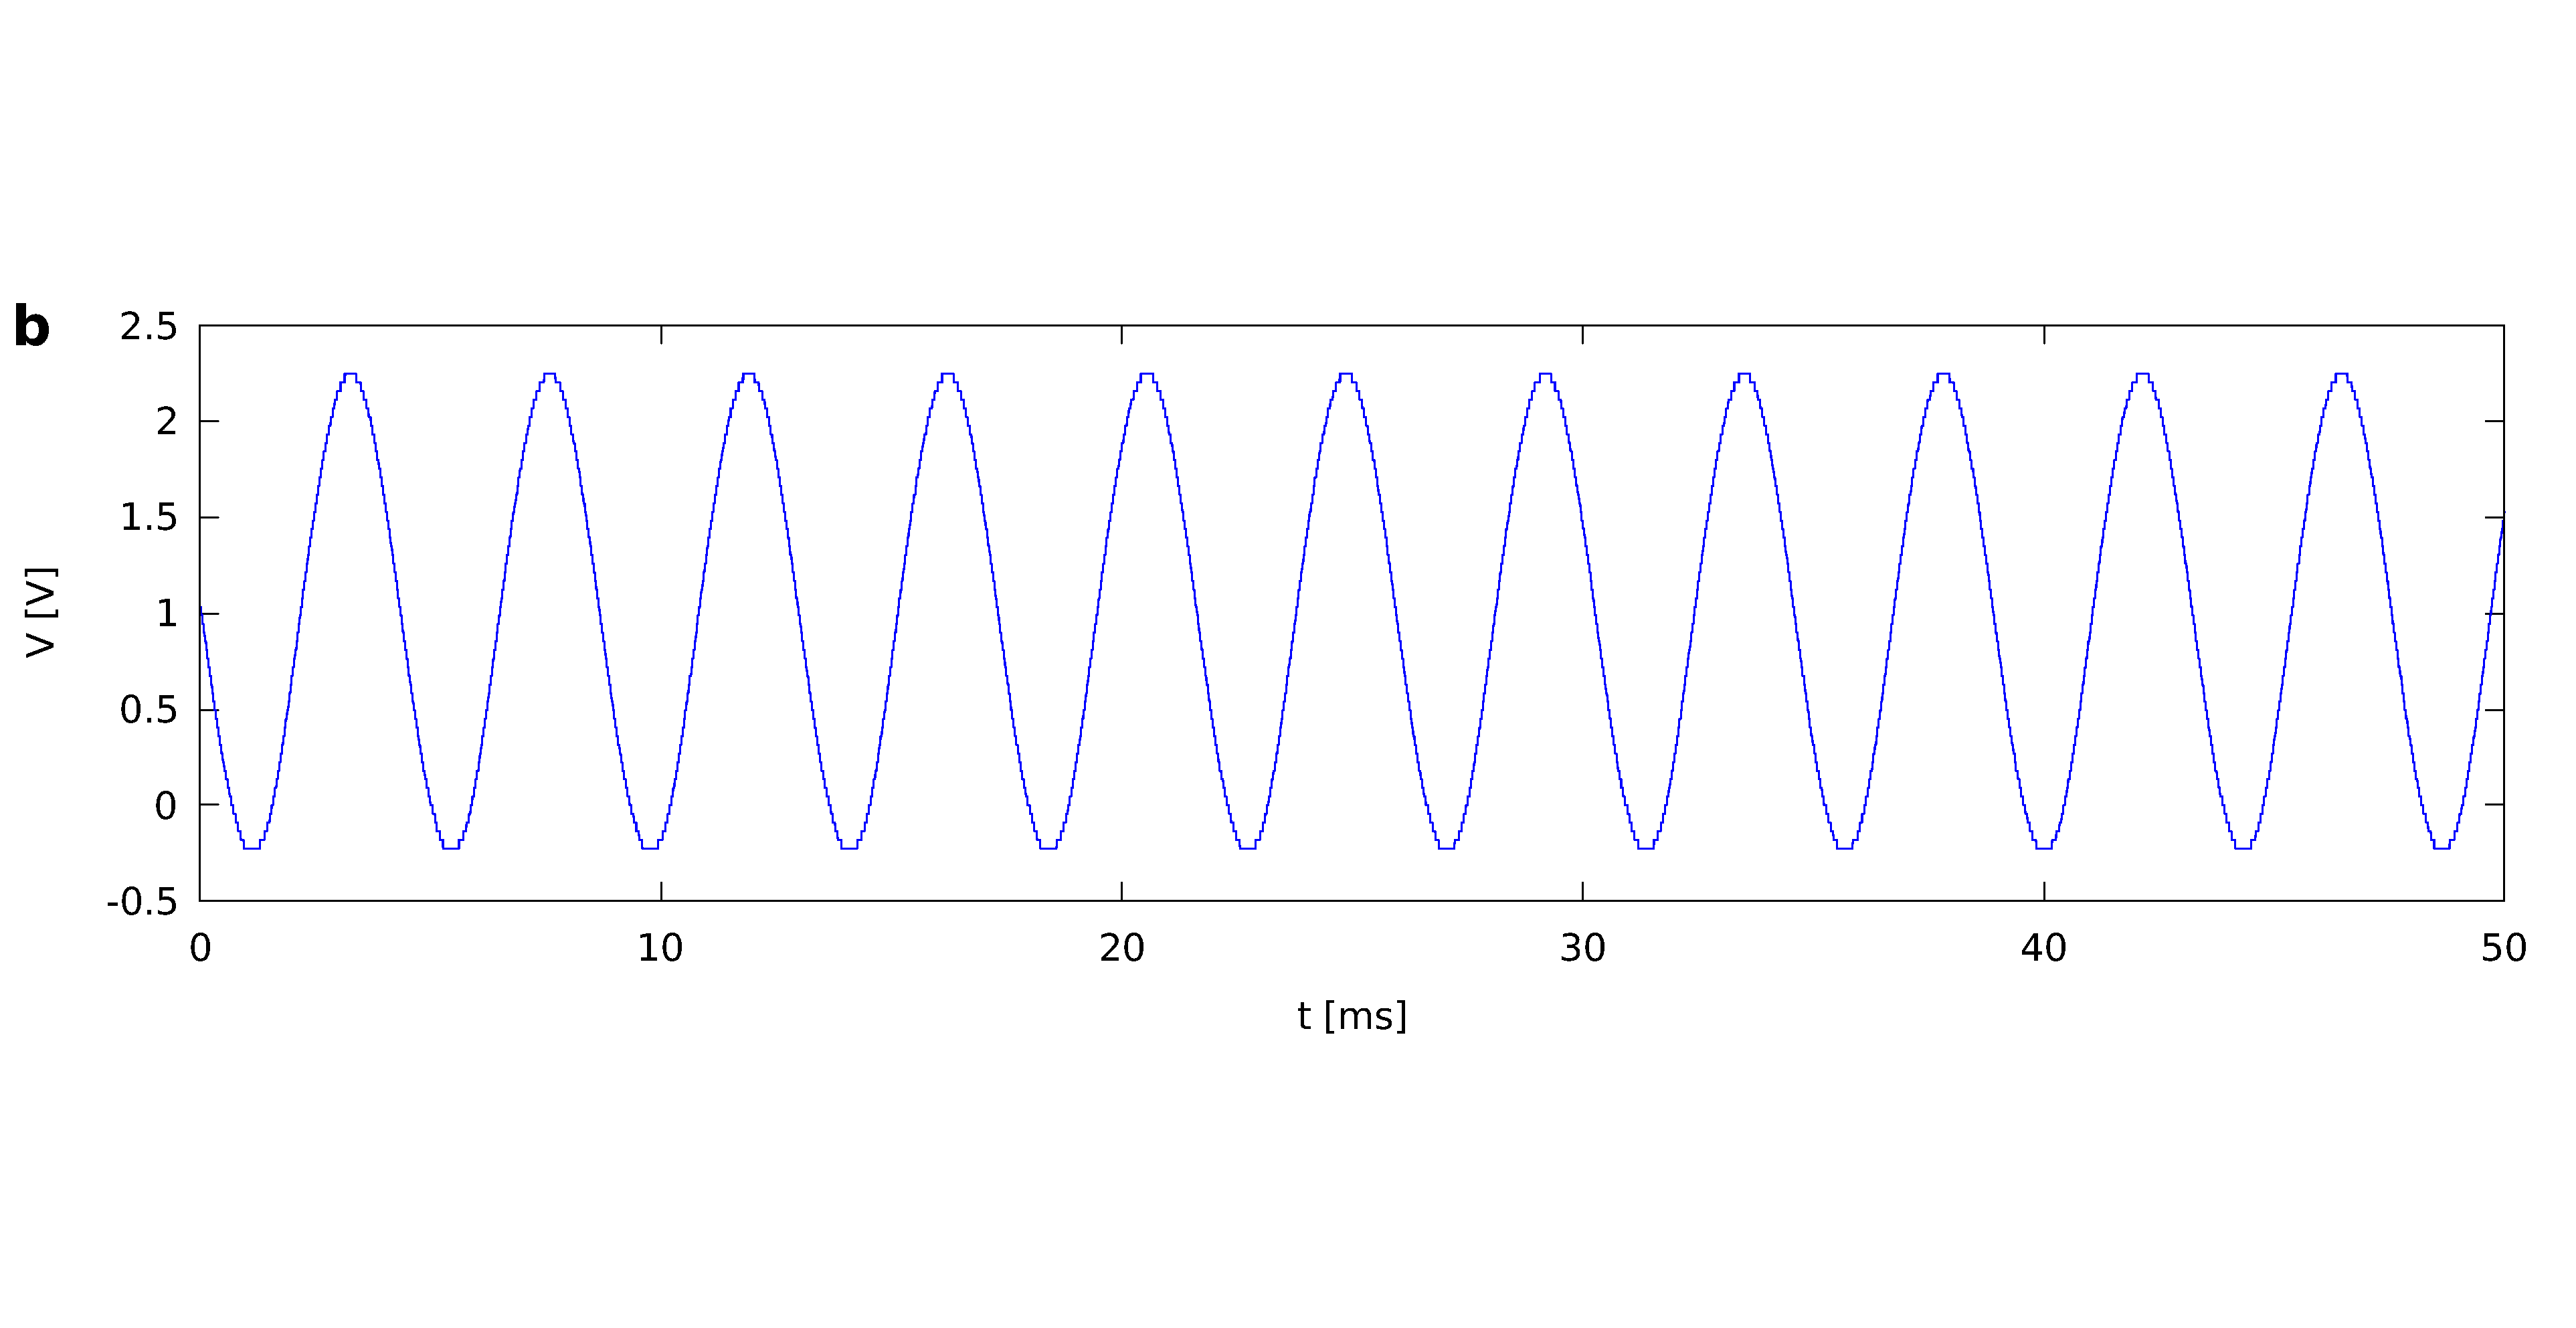
\includegraphics[width=\linewidth,trim={0 6cm 0 6cm},clip,left]
            {../1_block/prototypes/V_wf.pdf}
        \end{subfigure}
    \end{minipage}
    \begin{subfigure}{.39\textwidth}
        \centering
        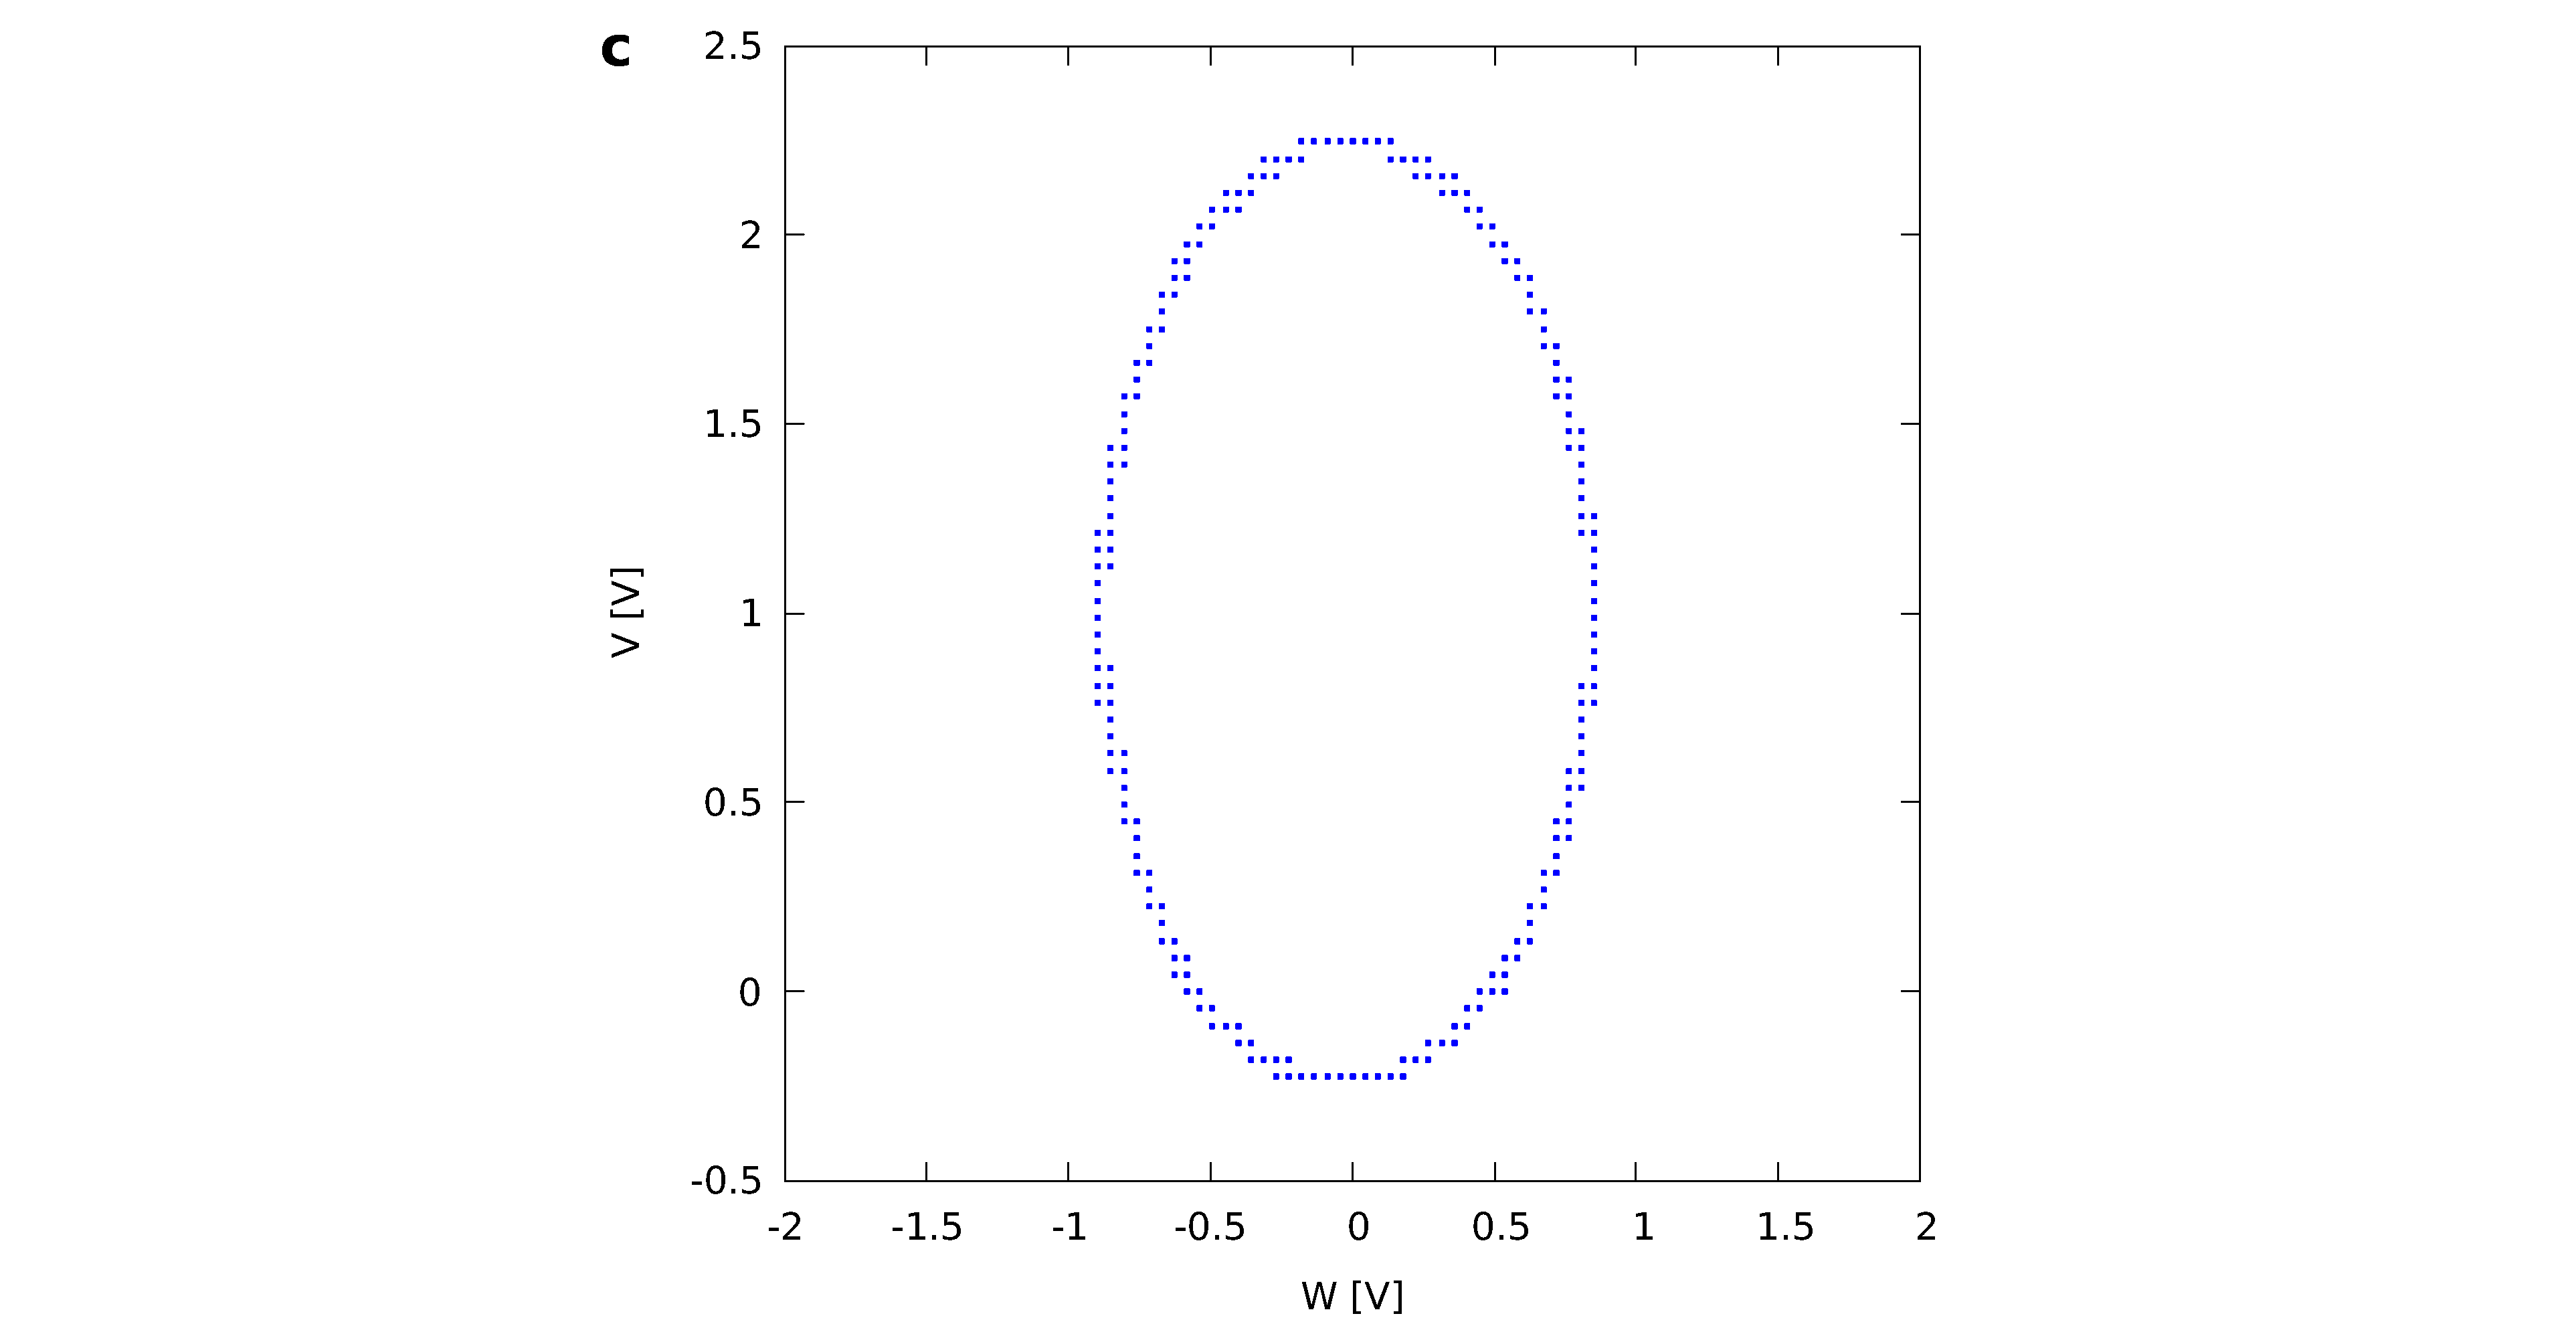
\includegraphics[width=\linewidth,trim={15cm 0 15cm 0},clip,right]
        {../1_block/prototypes/Lissajous.pdf}
    \end{subfigure}
    \begin{subfigure}{.49\textwidth}
        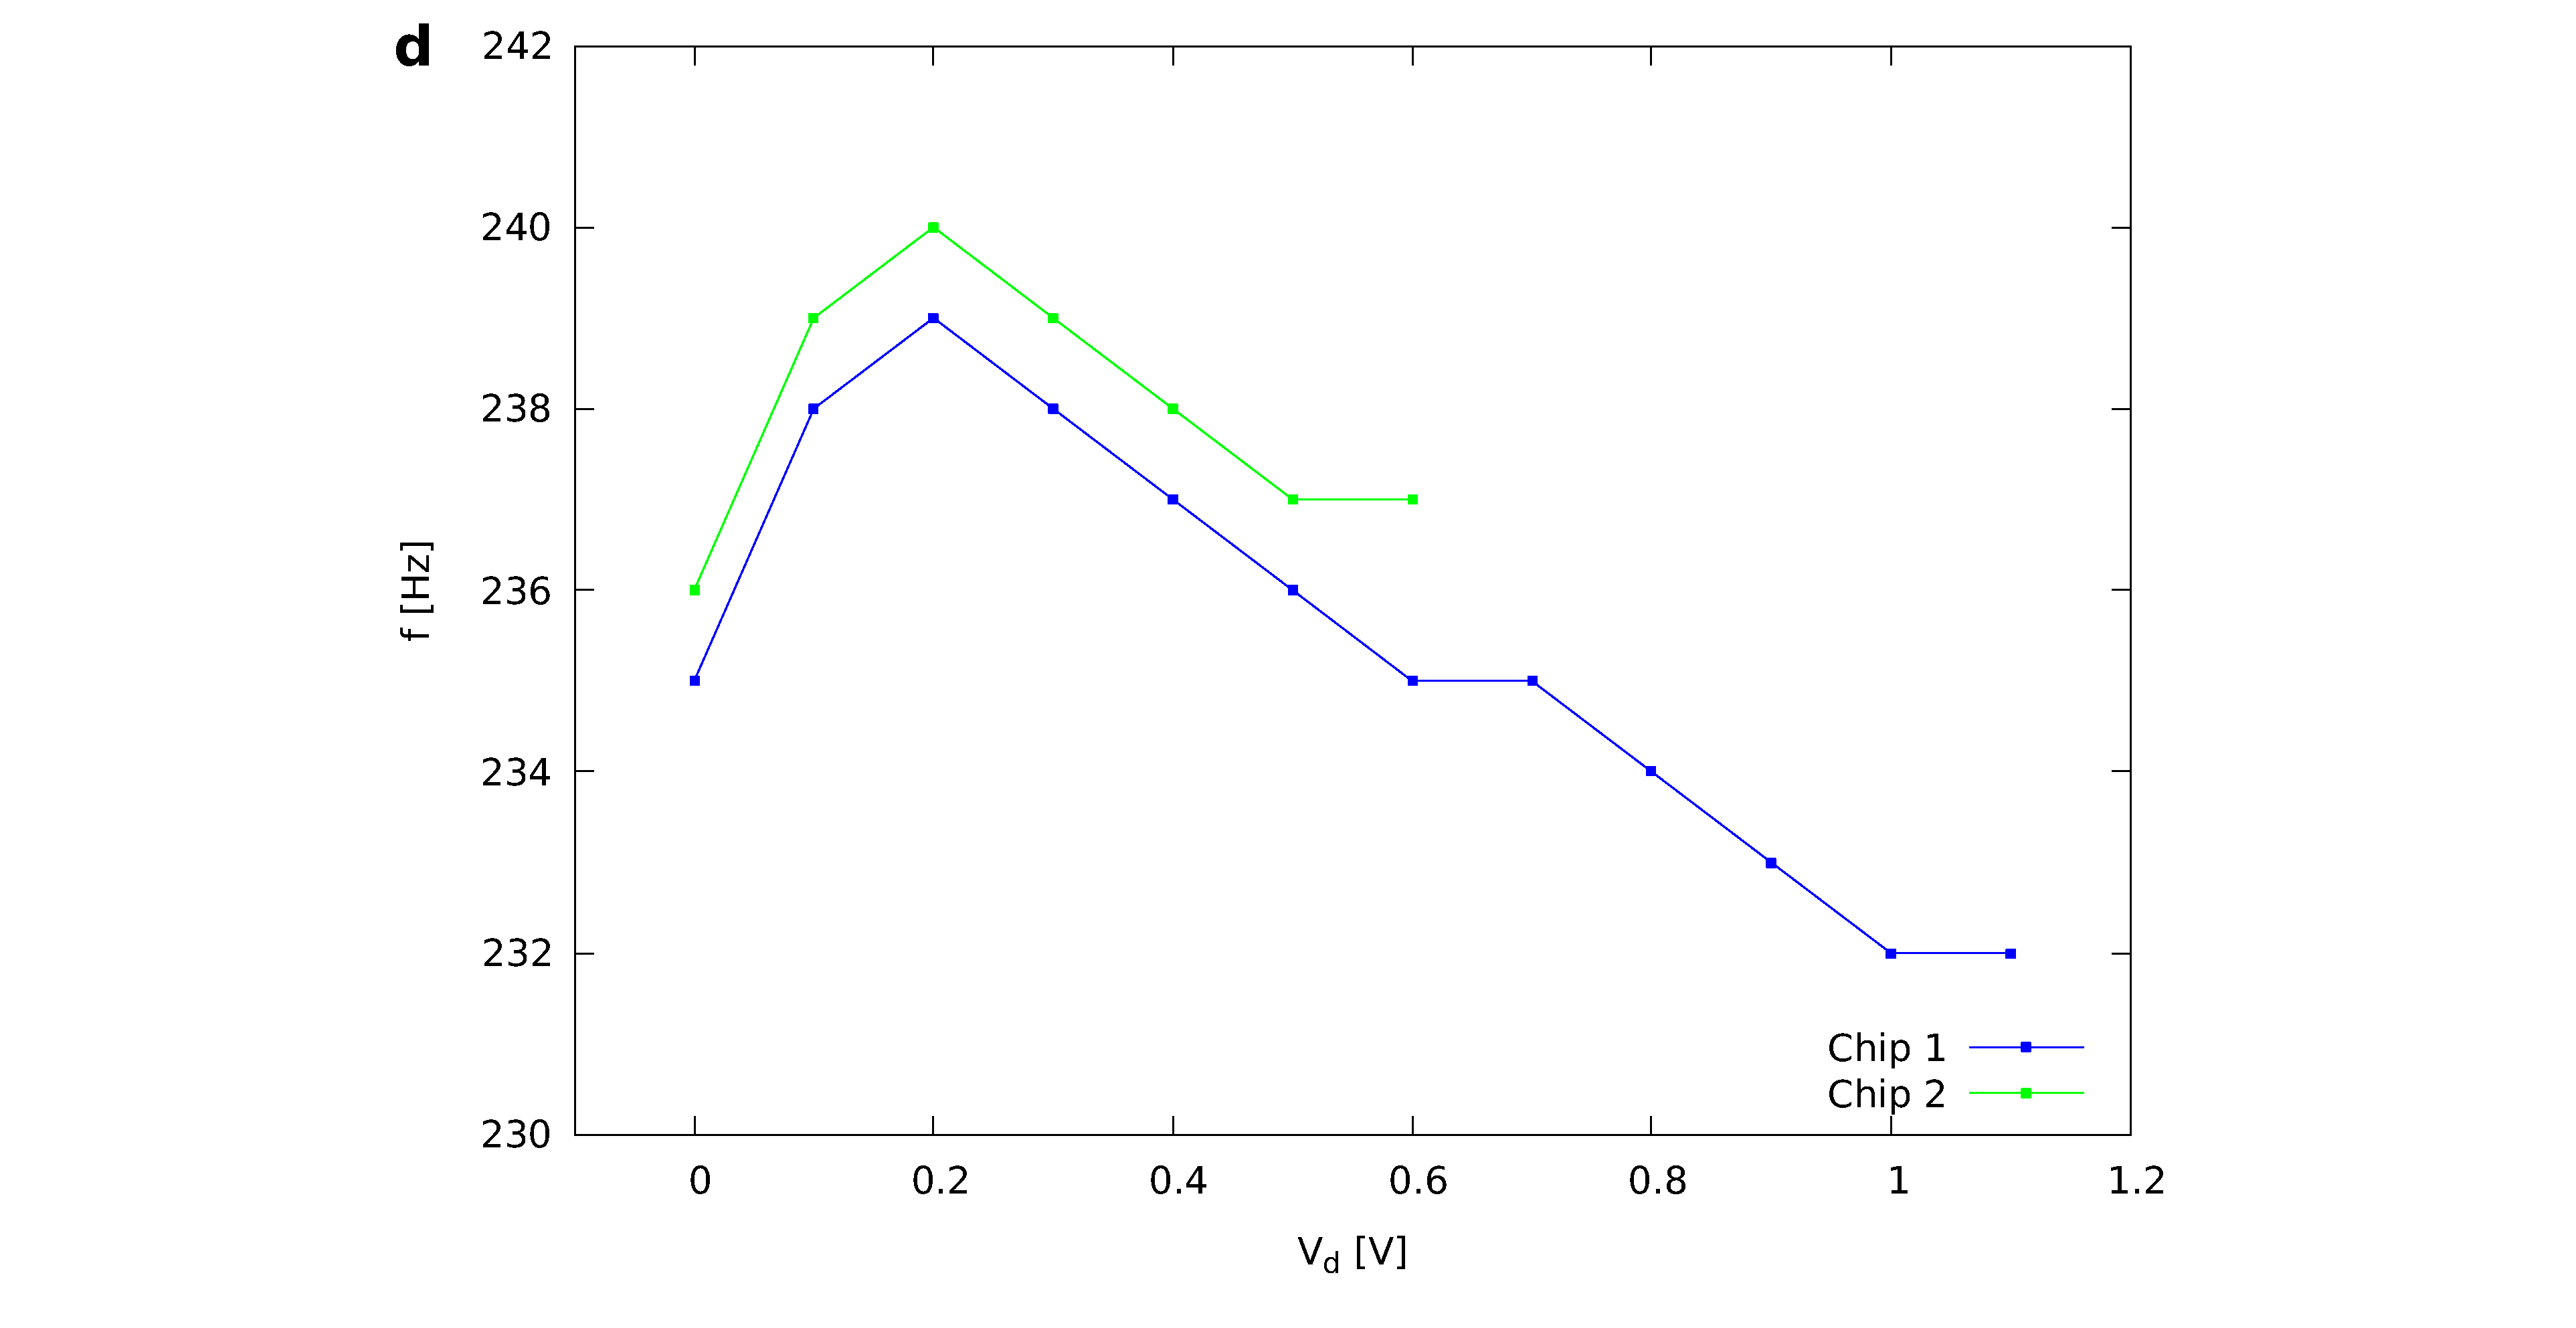
\includegraphics[width=\linewidth,trim={10cm 0 9cm 0},clip,left]
        {../1_block/prototypes/freq_prot.pdf}
    \end{subfigure}
    \begin{subfigure}{.49\textwidth}
        \centering
        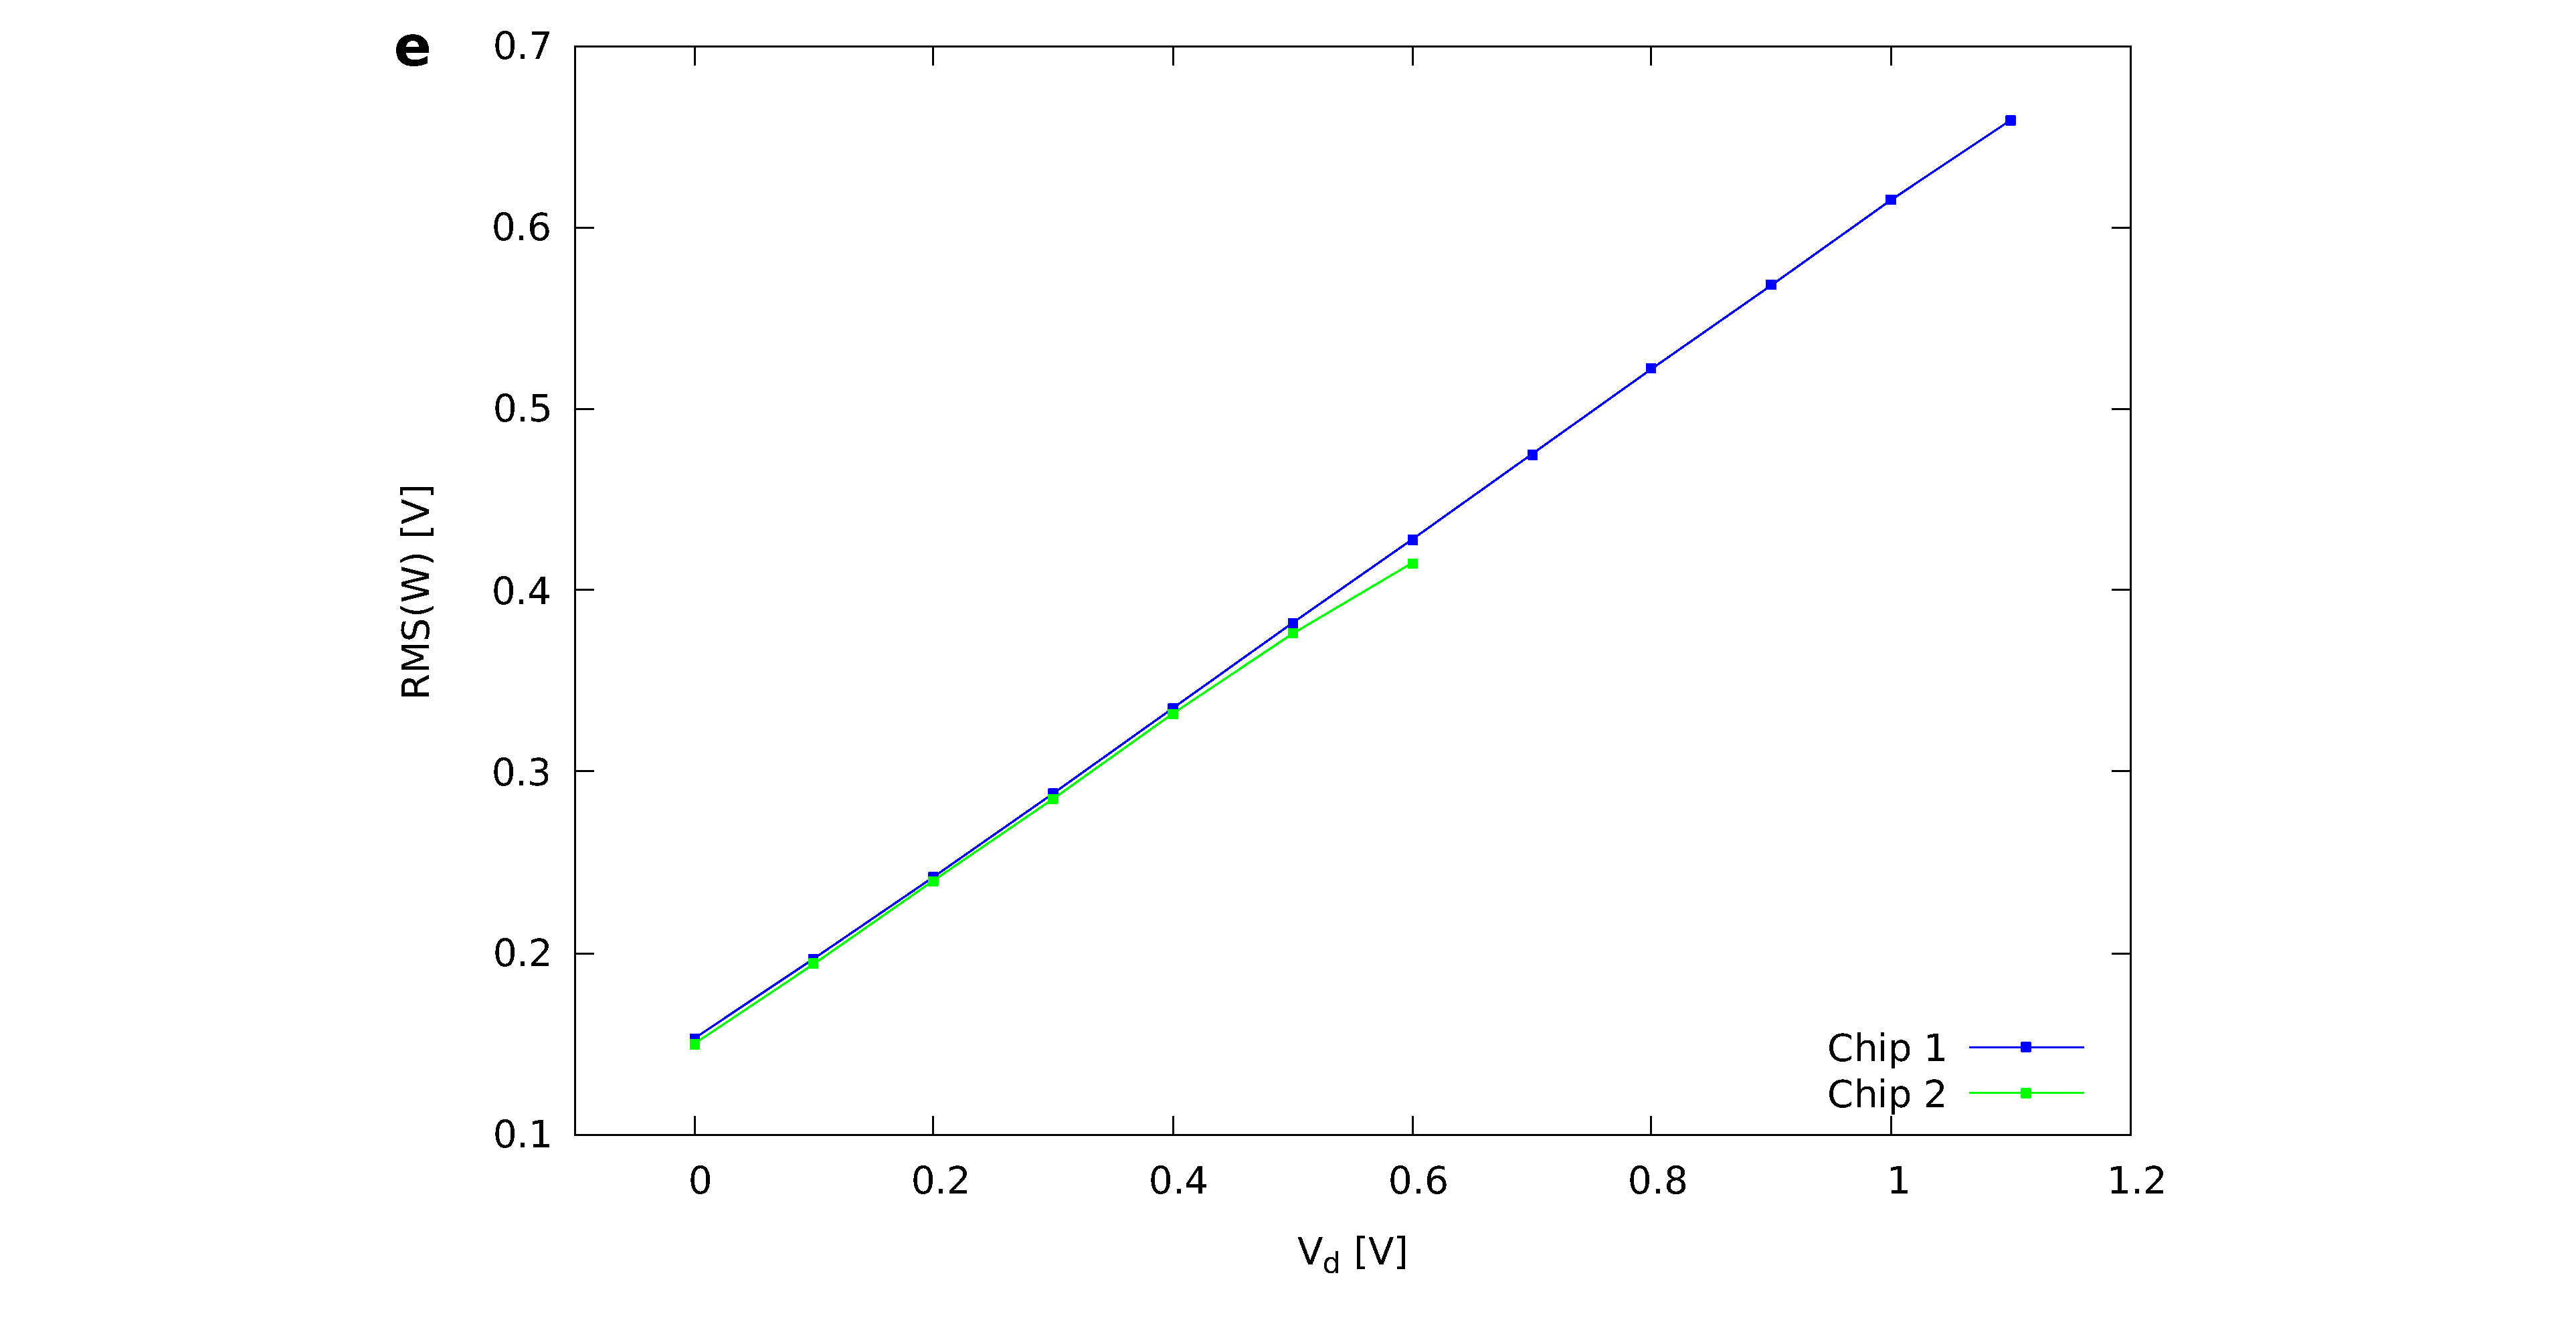
\includegraphics[width=\linewidth,trim={9cm 0 10cm 0},clip,right]
        {../1_block/prototypes/rms_prot.pdf}
    \end{subfigure}
    \caption{Oscillating behavior for the circuit implemented on
    the prototypical chips. (a) Plot of $W$ and (b) of $V$ as a
    function of time, for $V_d=1$ V.
    (c) Phase portrait (Lissajous figure) of $V$ versus $W$. (d)
    Frequency and (e) root mean square amplitude of the
    output signal $W$ as a function of the parameter $V_d$ and for
    the two different chips.}
    \label{fig:oscillation prototype}
\end{figure}

\section{Board}\label{sec:board}

In order to finally analyze the behavior of many coupled
oscillators, a board containing 25 chips (or blocks) has been built.
The circuit diagram is equivalent to the one shown in Fig.
\ref{fig:prototype implementation} for the prototypes, the only
difference being the use of DFLS1100 Schottky diodes instead of
MBRA210L ones.

The oscillating behavior is shown in Fig.
\ref{fig:oscillation board}. Once again, these systems are not as
stable as the circuit on the breadboard; measurements were in fact
taken for $V_d \leq 2.2$ V for the first two blocks. It is important to notice
that in the voltage range $0.6~\text{V} \leq V_d \leq 2.1~\text{V}$
a clamping of the output voltage $V$ can be observed; this is not
intended and is probably due to intrinsic limitations in the current.

\begin{figure}[H]
    \centering
    \begin{minipage}{.58\textwidth}
        \begin{subfigure}{\linewidth}
            \centering
            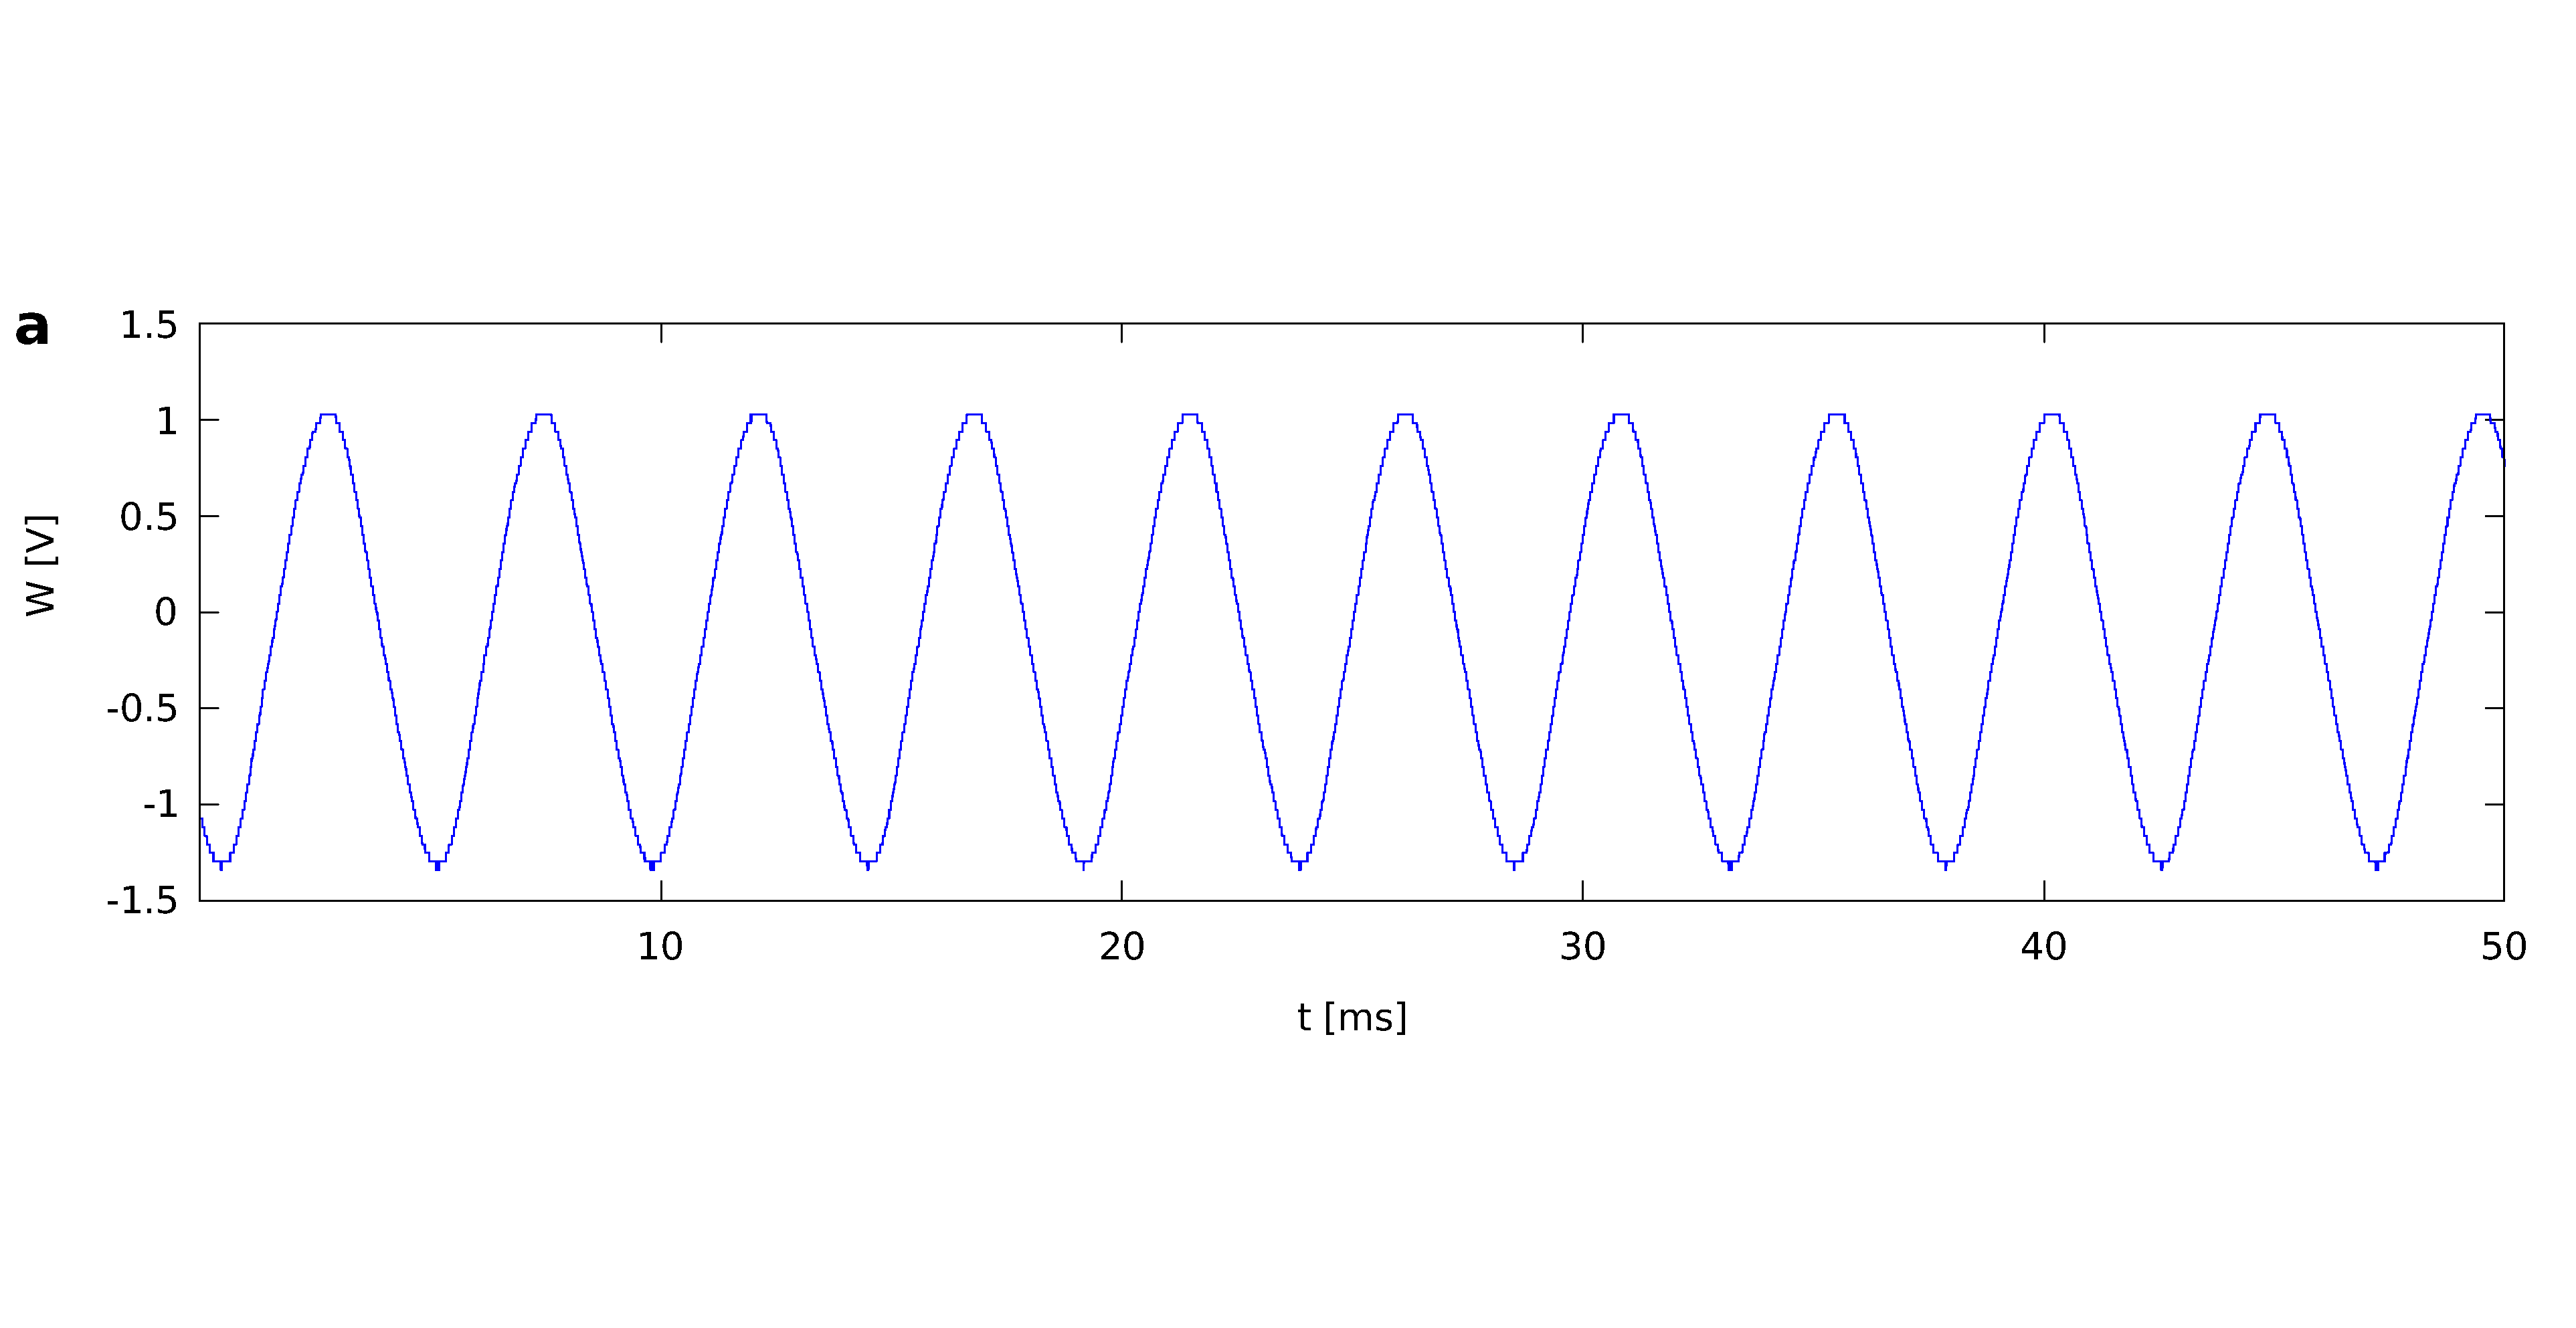
\includegraphics[width=\linewidth,trim={0 6cm 0 6cm},clip,left]
            {../1_block/board/W_wf.pdf}\\
            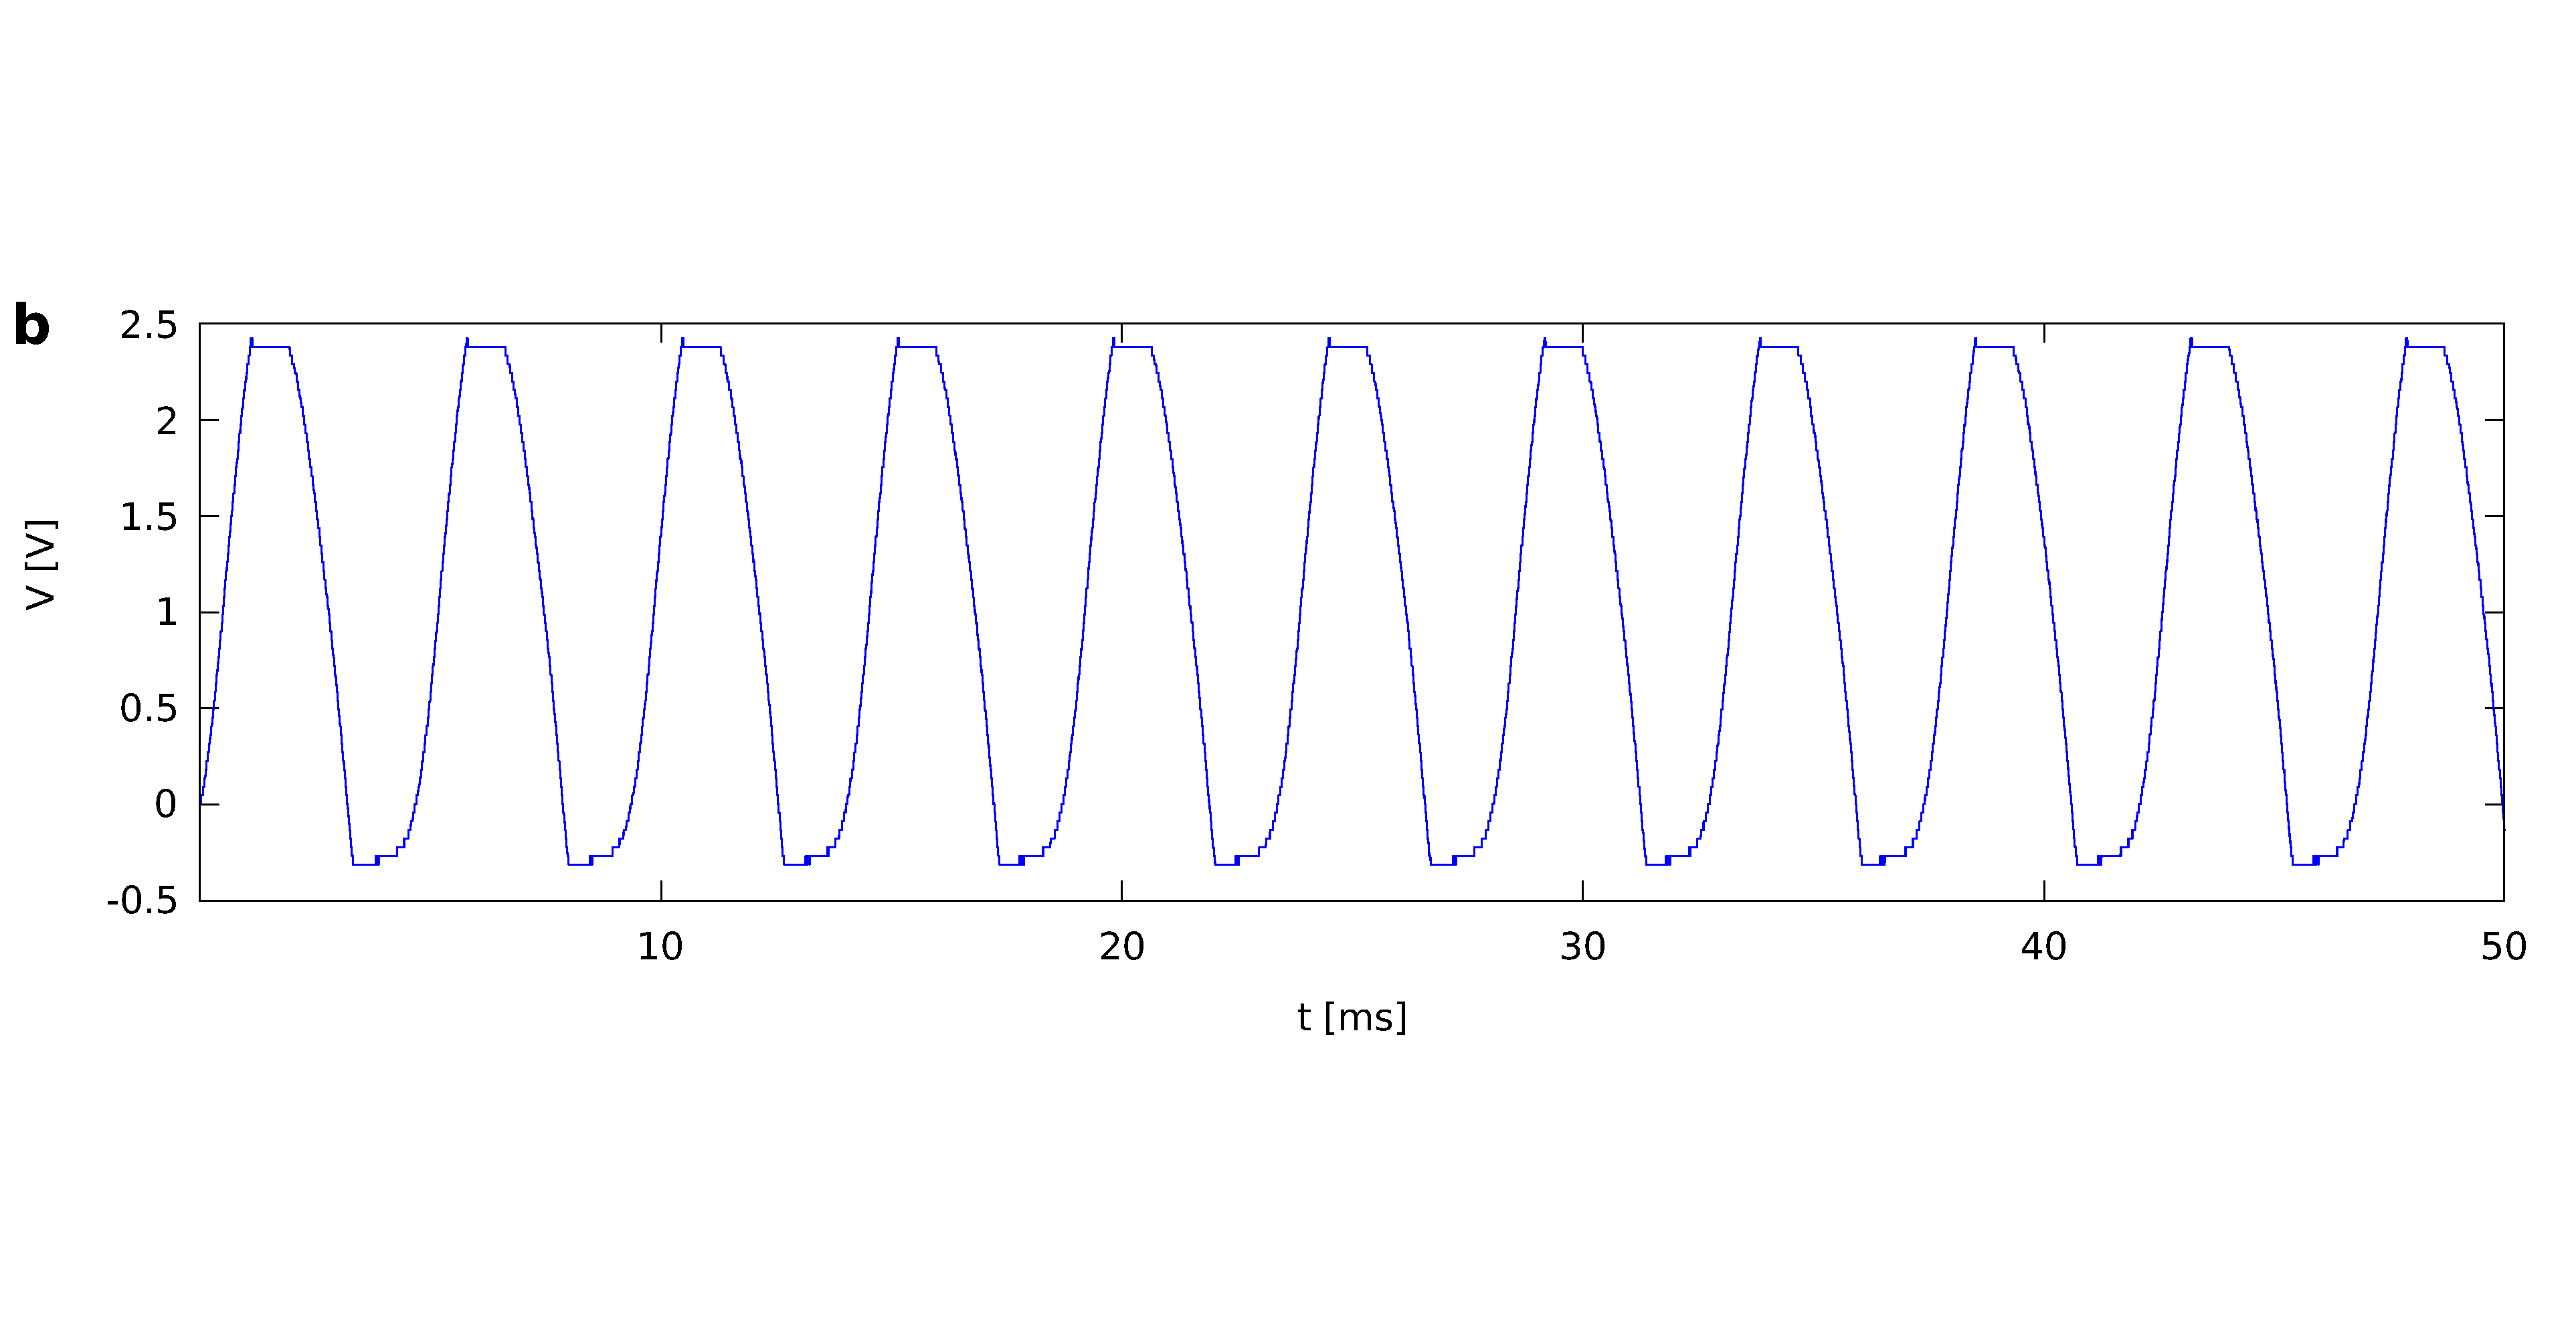
\includegraphics[width=\linewidth,trim={0 6cm 0 6cm},clip,left]
            {../1_block/board/V_wf.pdf}
        \end{subfigure}
    \end{minipage}
    \begin{subfigure}{.39\textwidth}
        \centering
        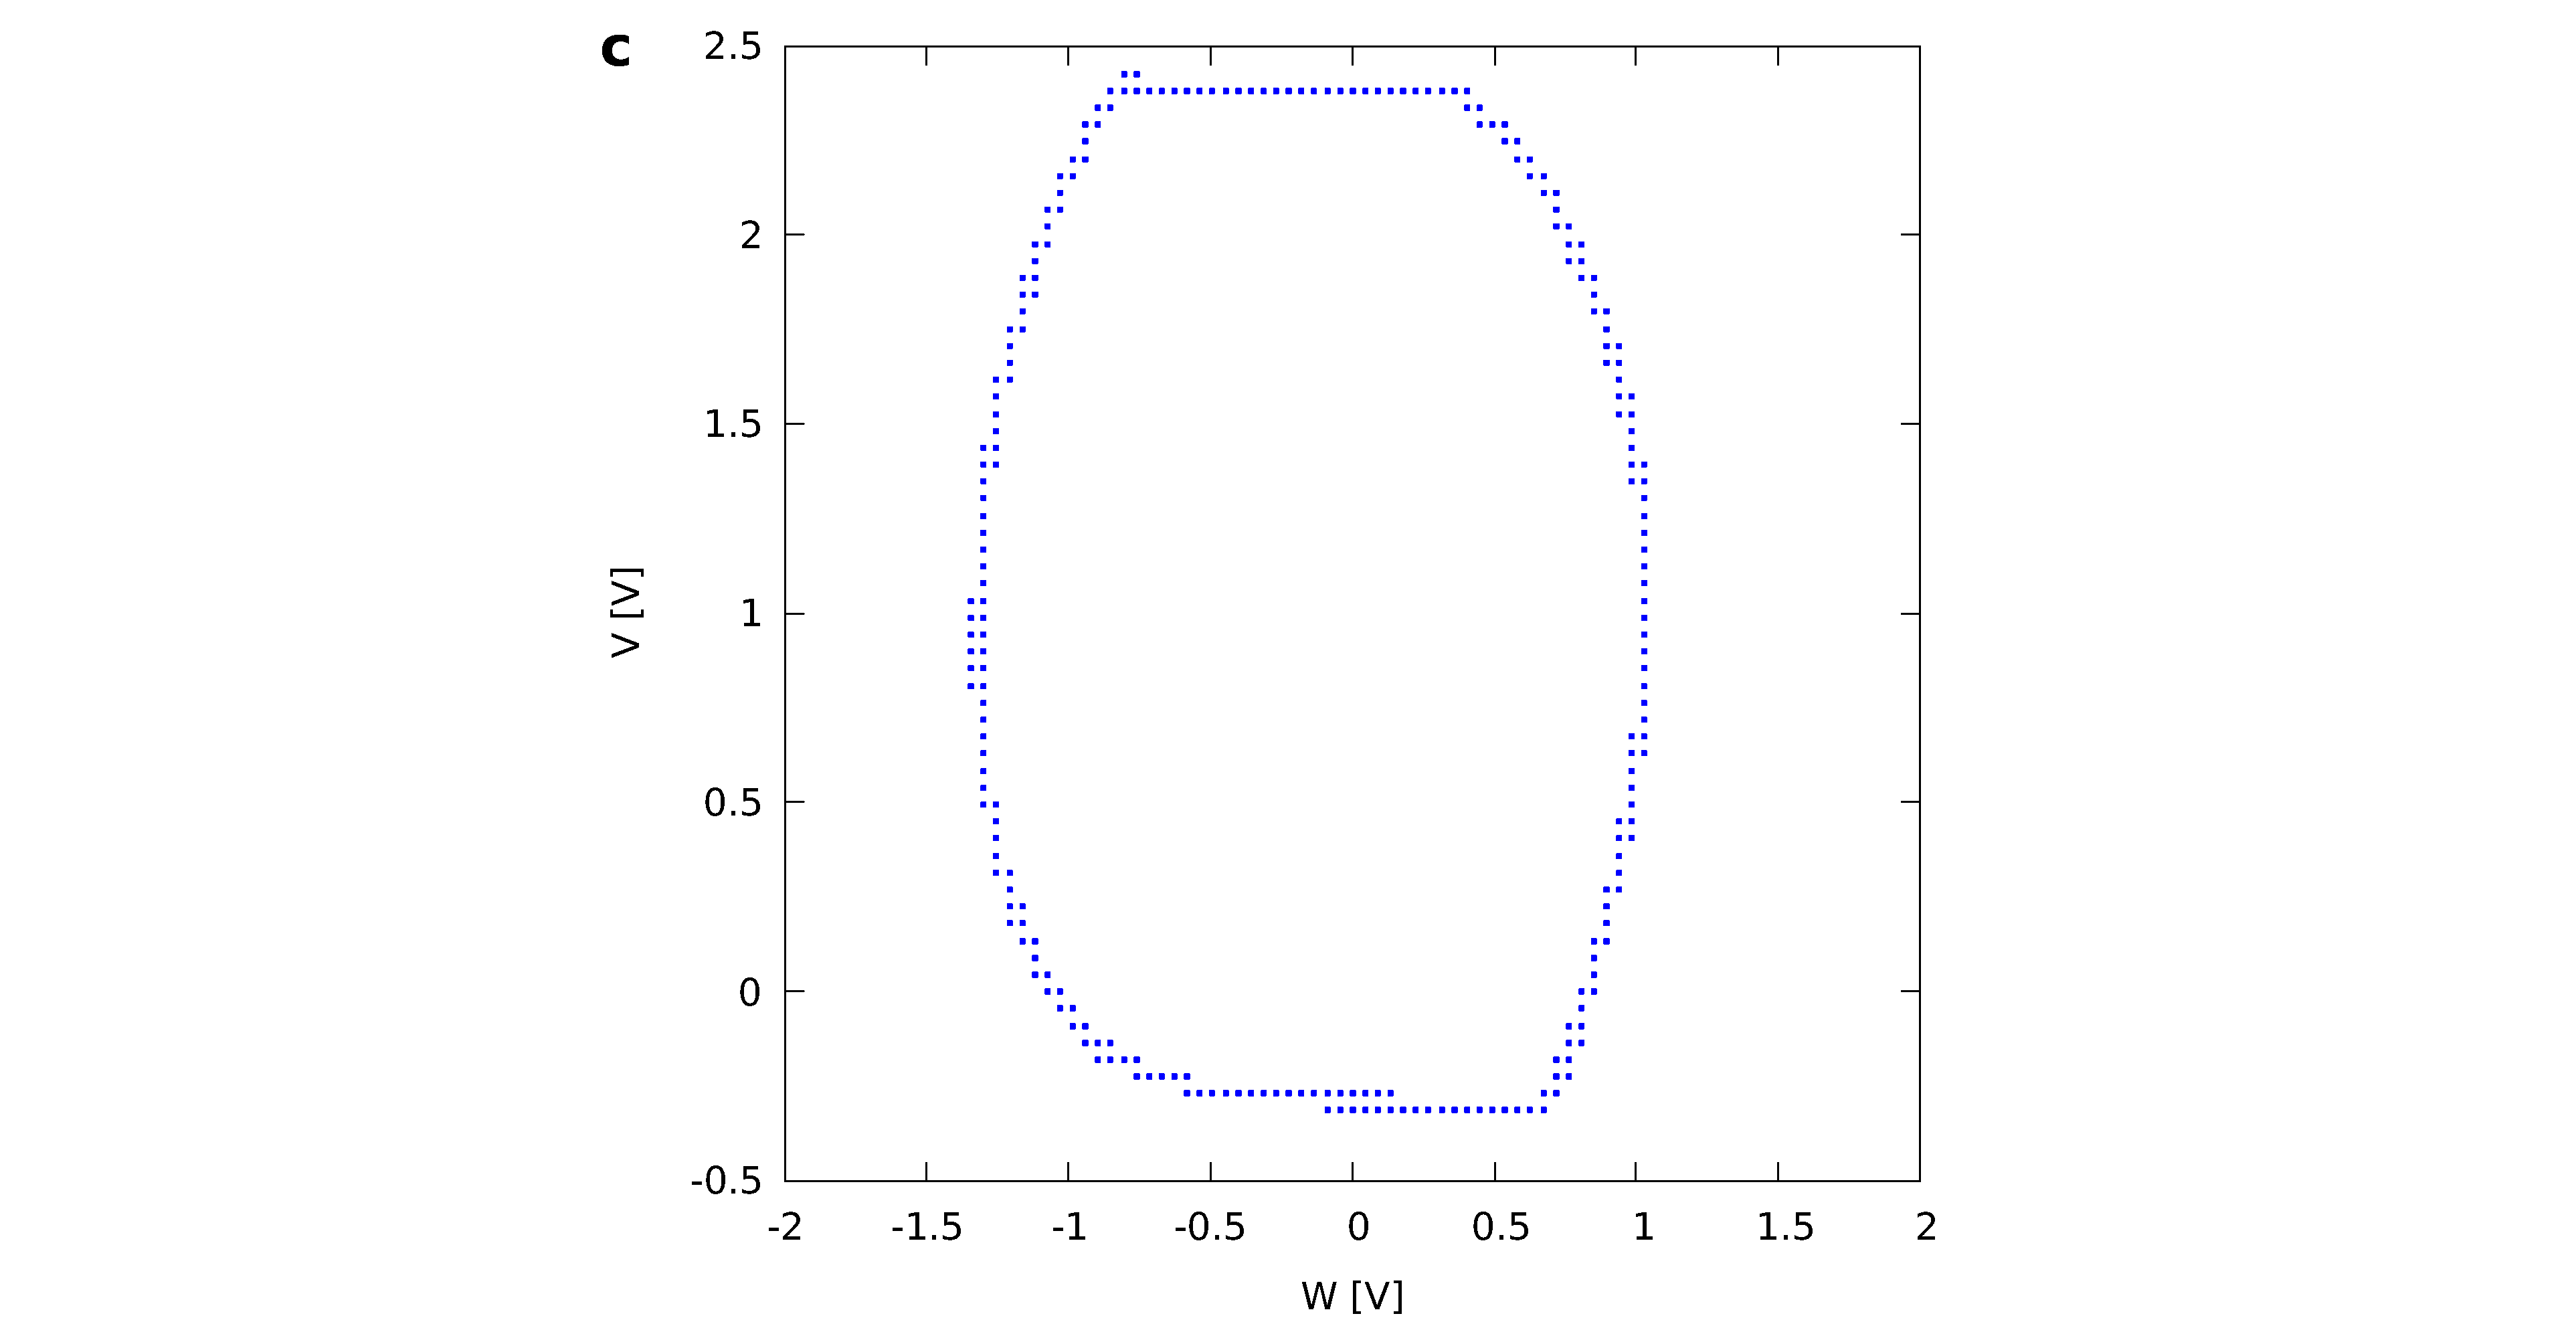
\includegraphics[width=\linewidth,trim={15cm 0 15cm 0},clip,right]
        {../1_block/board/Lissajous.pdf}
    \end{subfigure}
    \begin{subfigure}{.49\textwidth}
        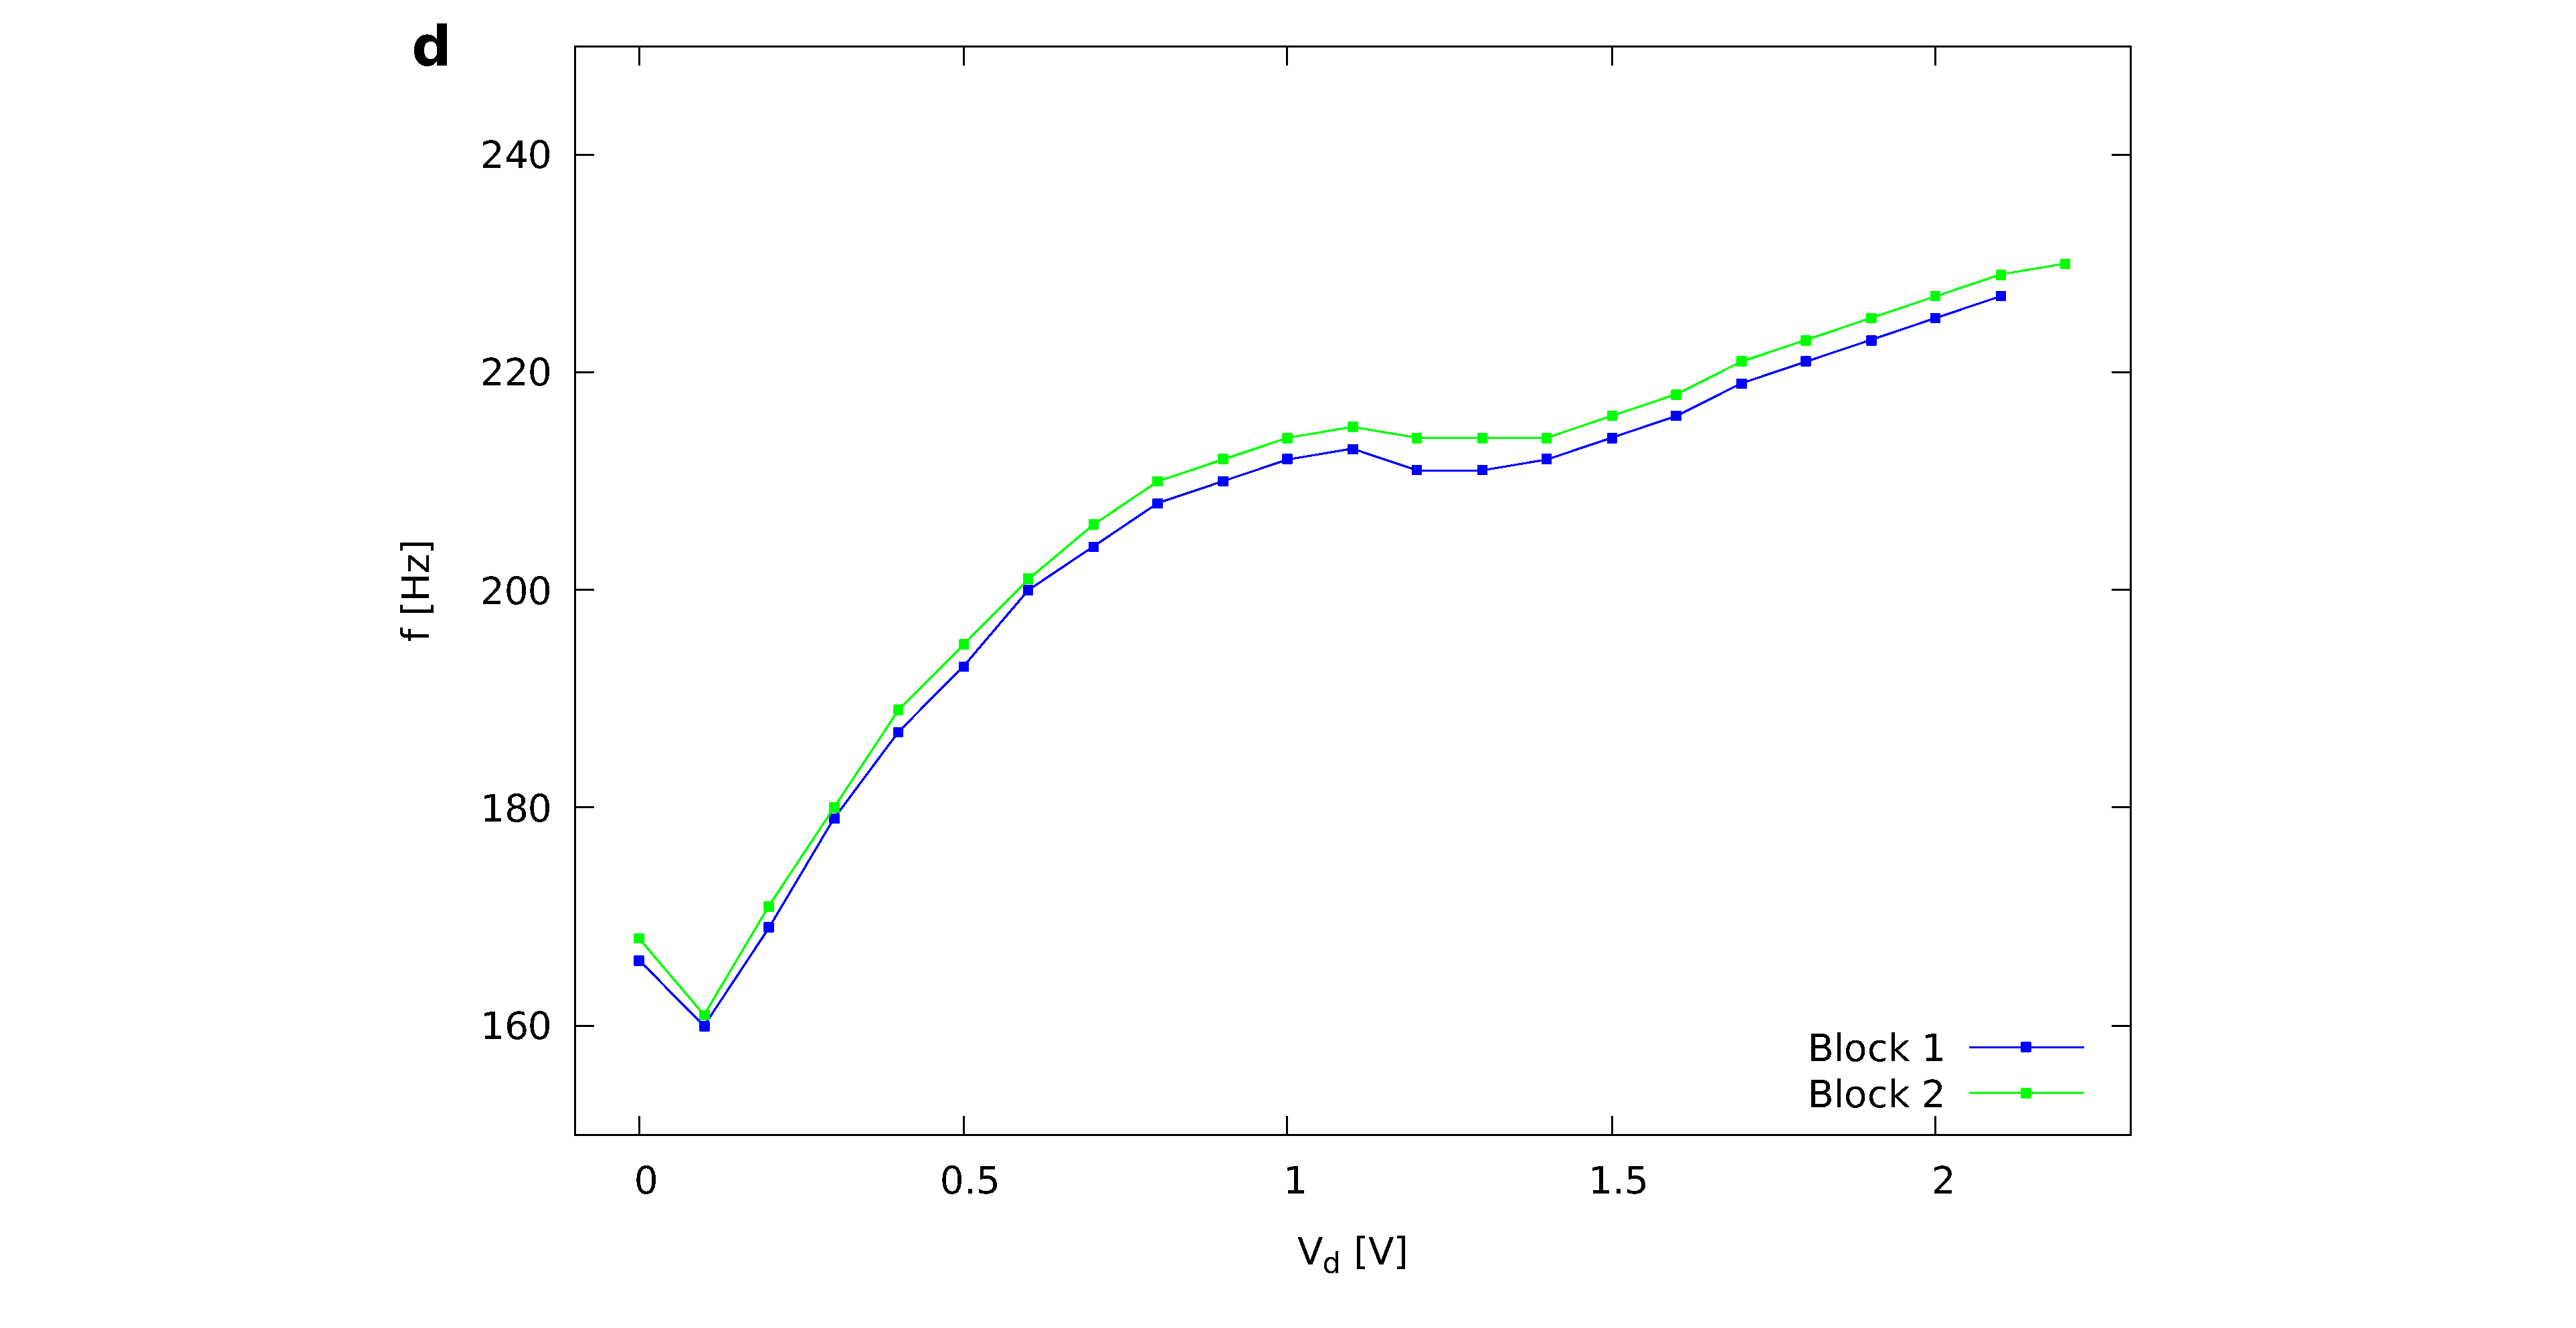
\includegraphics[width=\linewidth,trim={10cm 0 9cm 0},clip,left]
        {../1_block/board/freq_board.pdf}
    \end{subfigure}
    \begin{subfigure}{.49\textwidth}
        \centering
        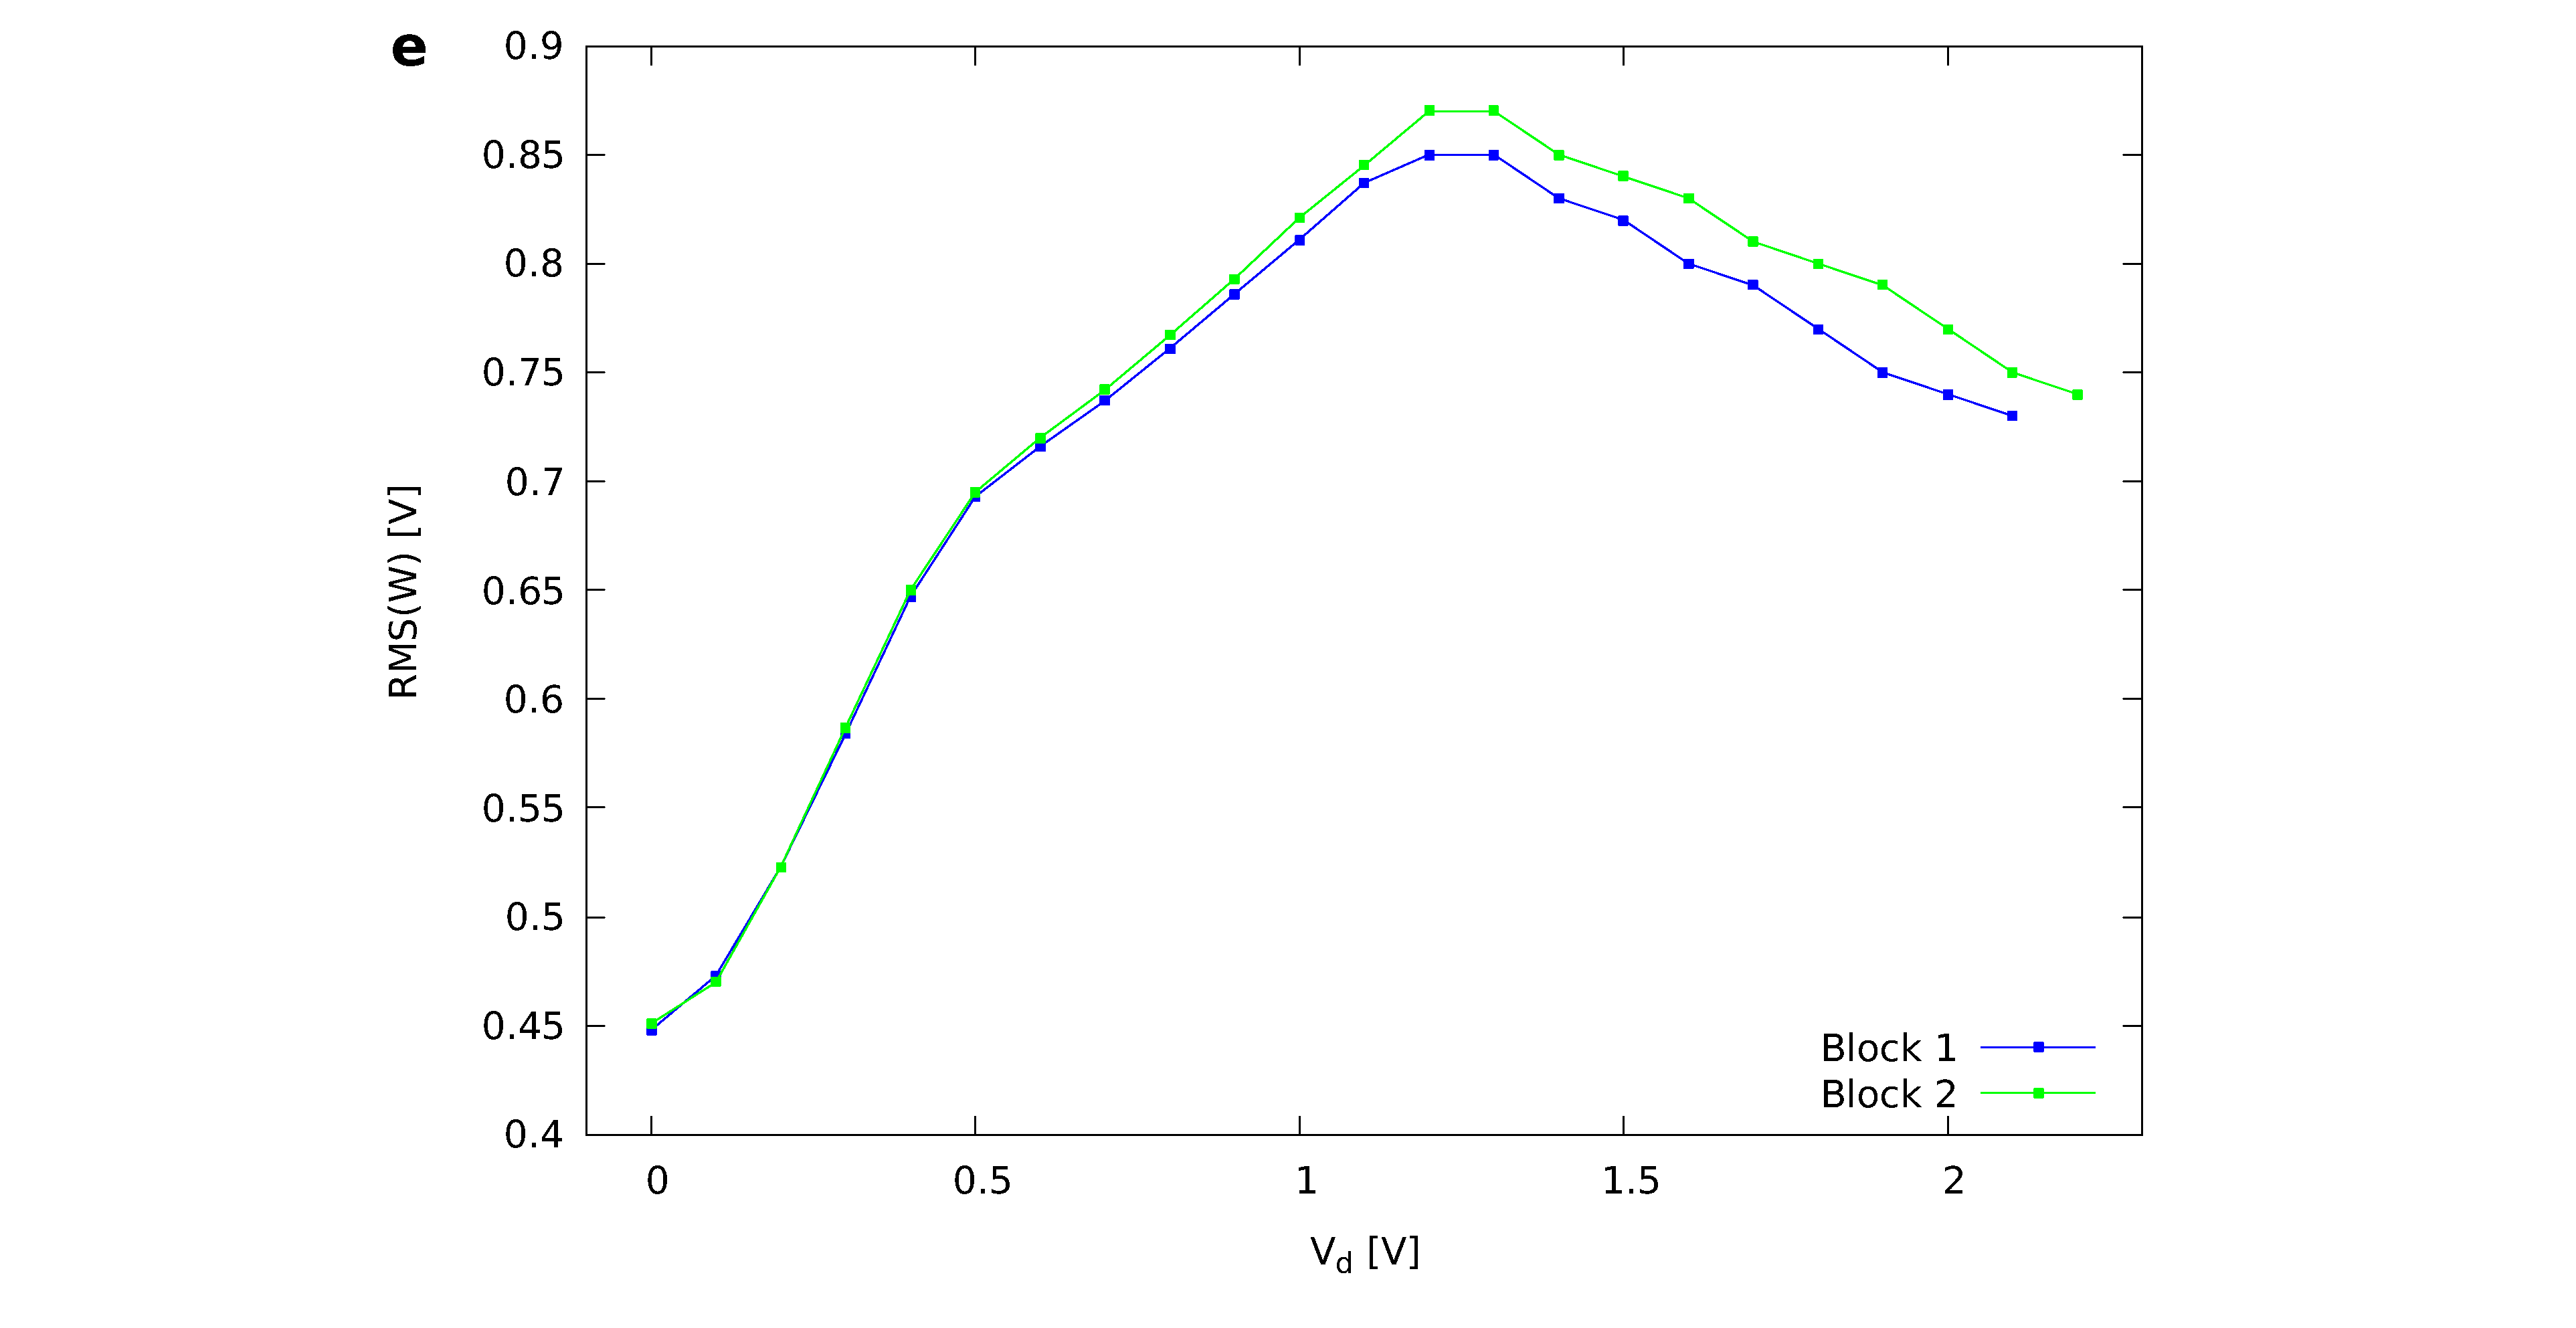
\includegraphics[width=\linewidth,trim={9cm 0 10cm 0},clip,right]
        {../1_block/board/rms_board.pdf}
    \end{subfigure}
    \caption{Oscillating behavior for the circuit implemented on
    the board. (a) Plot of $W$ and (b) of $V$ as a
    function of time, for $V_d=1$ V.
    (c) Phase portrait (Lissajous figure) of $V$ versus $W$. (d)
    Frequency and (e) root mean square amplitude of the
    output signal $W$ as a function of the parameter $V_d$ and for
    two different blocks.}
    \label{fig:oscillation board}
\end{figure}


\section{New board}\label{sec:new board}

\begin{figure}[H]
    \centering
    \begin{minipage}{.58\textwidth}
        \begin{subfigure}{\linewidth}
            \centering
            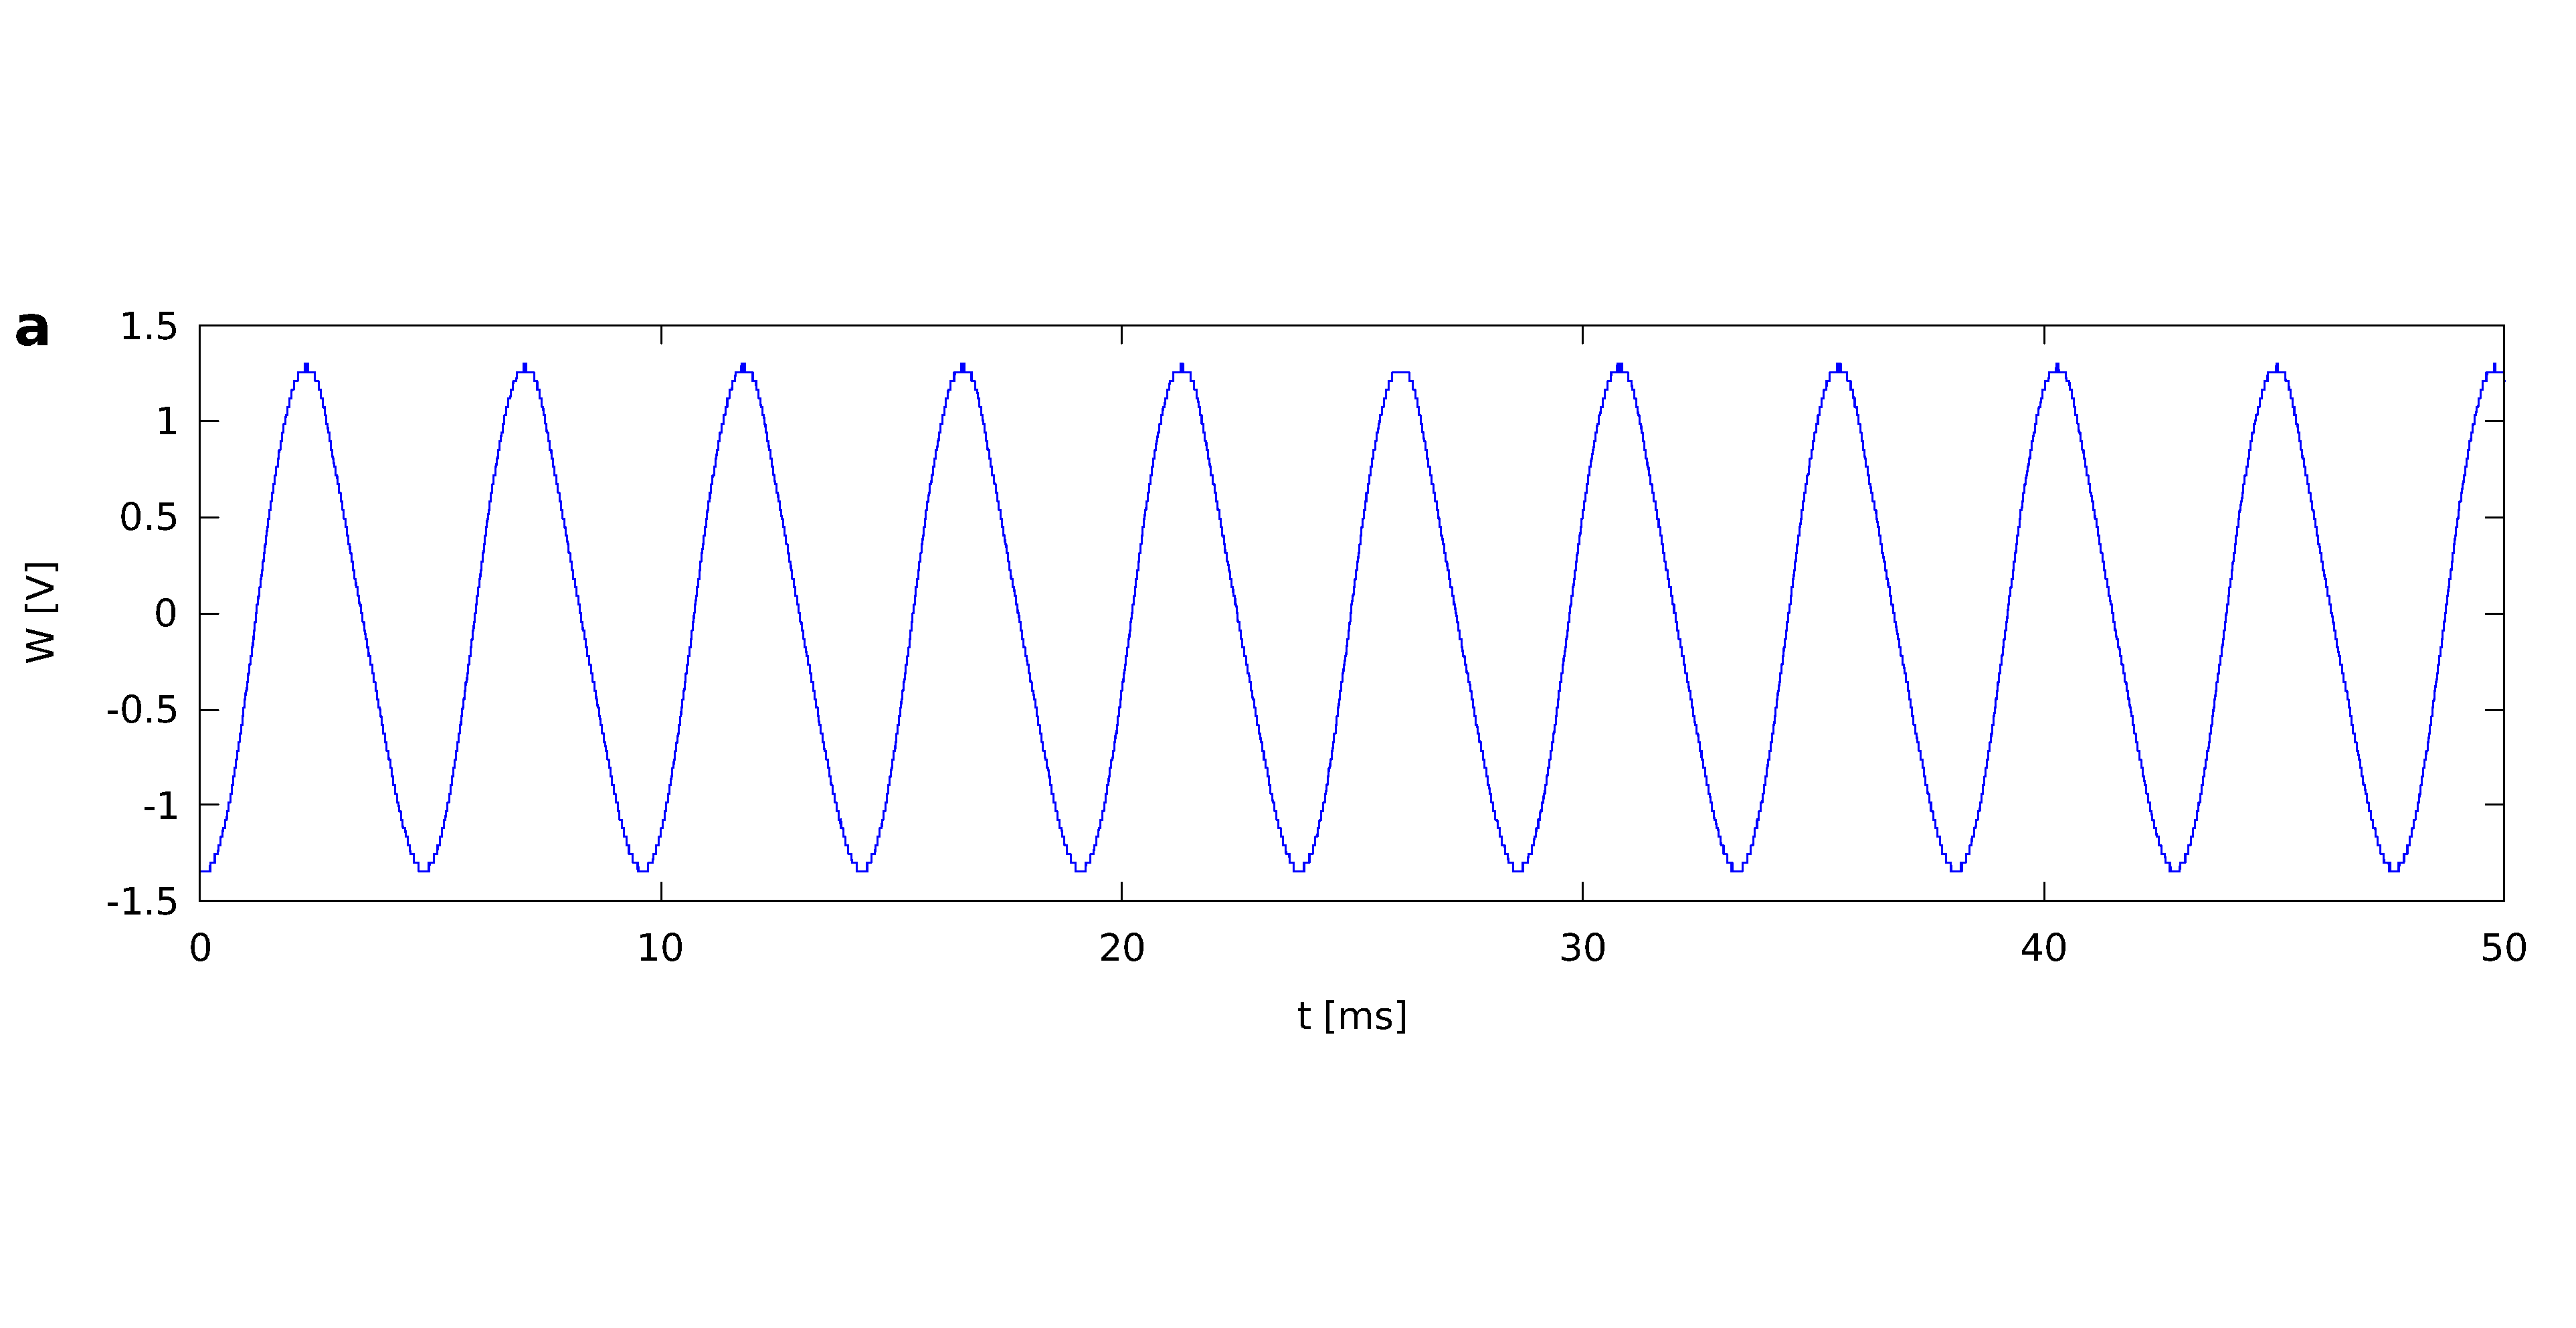
\includegraphics[width=\linewidth,trim={0 6cm 0 6cm},clip,left]
            {../1_block/board_new/W_wf.pdf}\\
            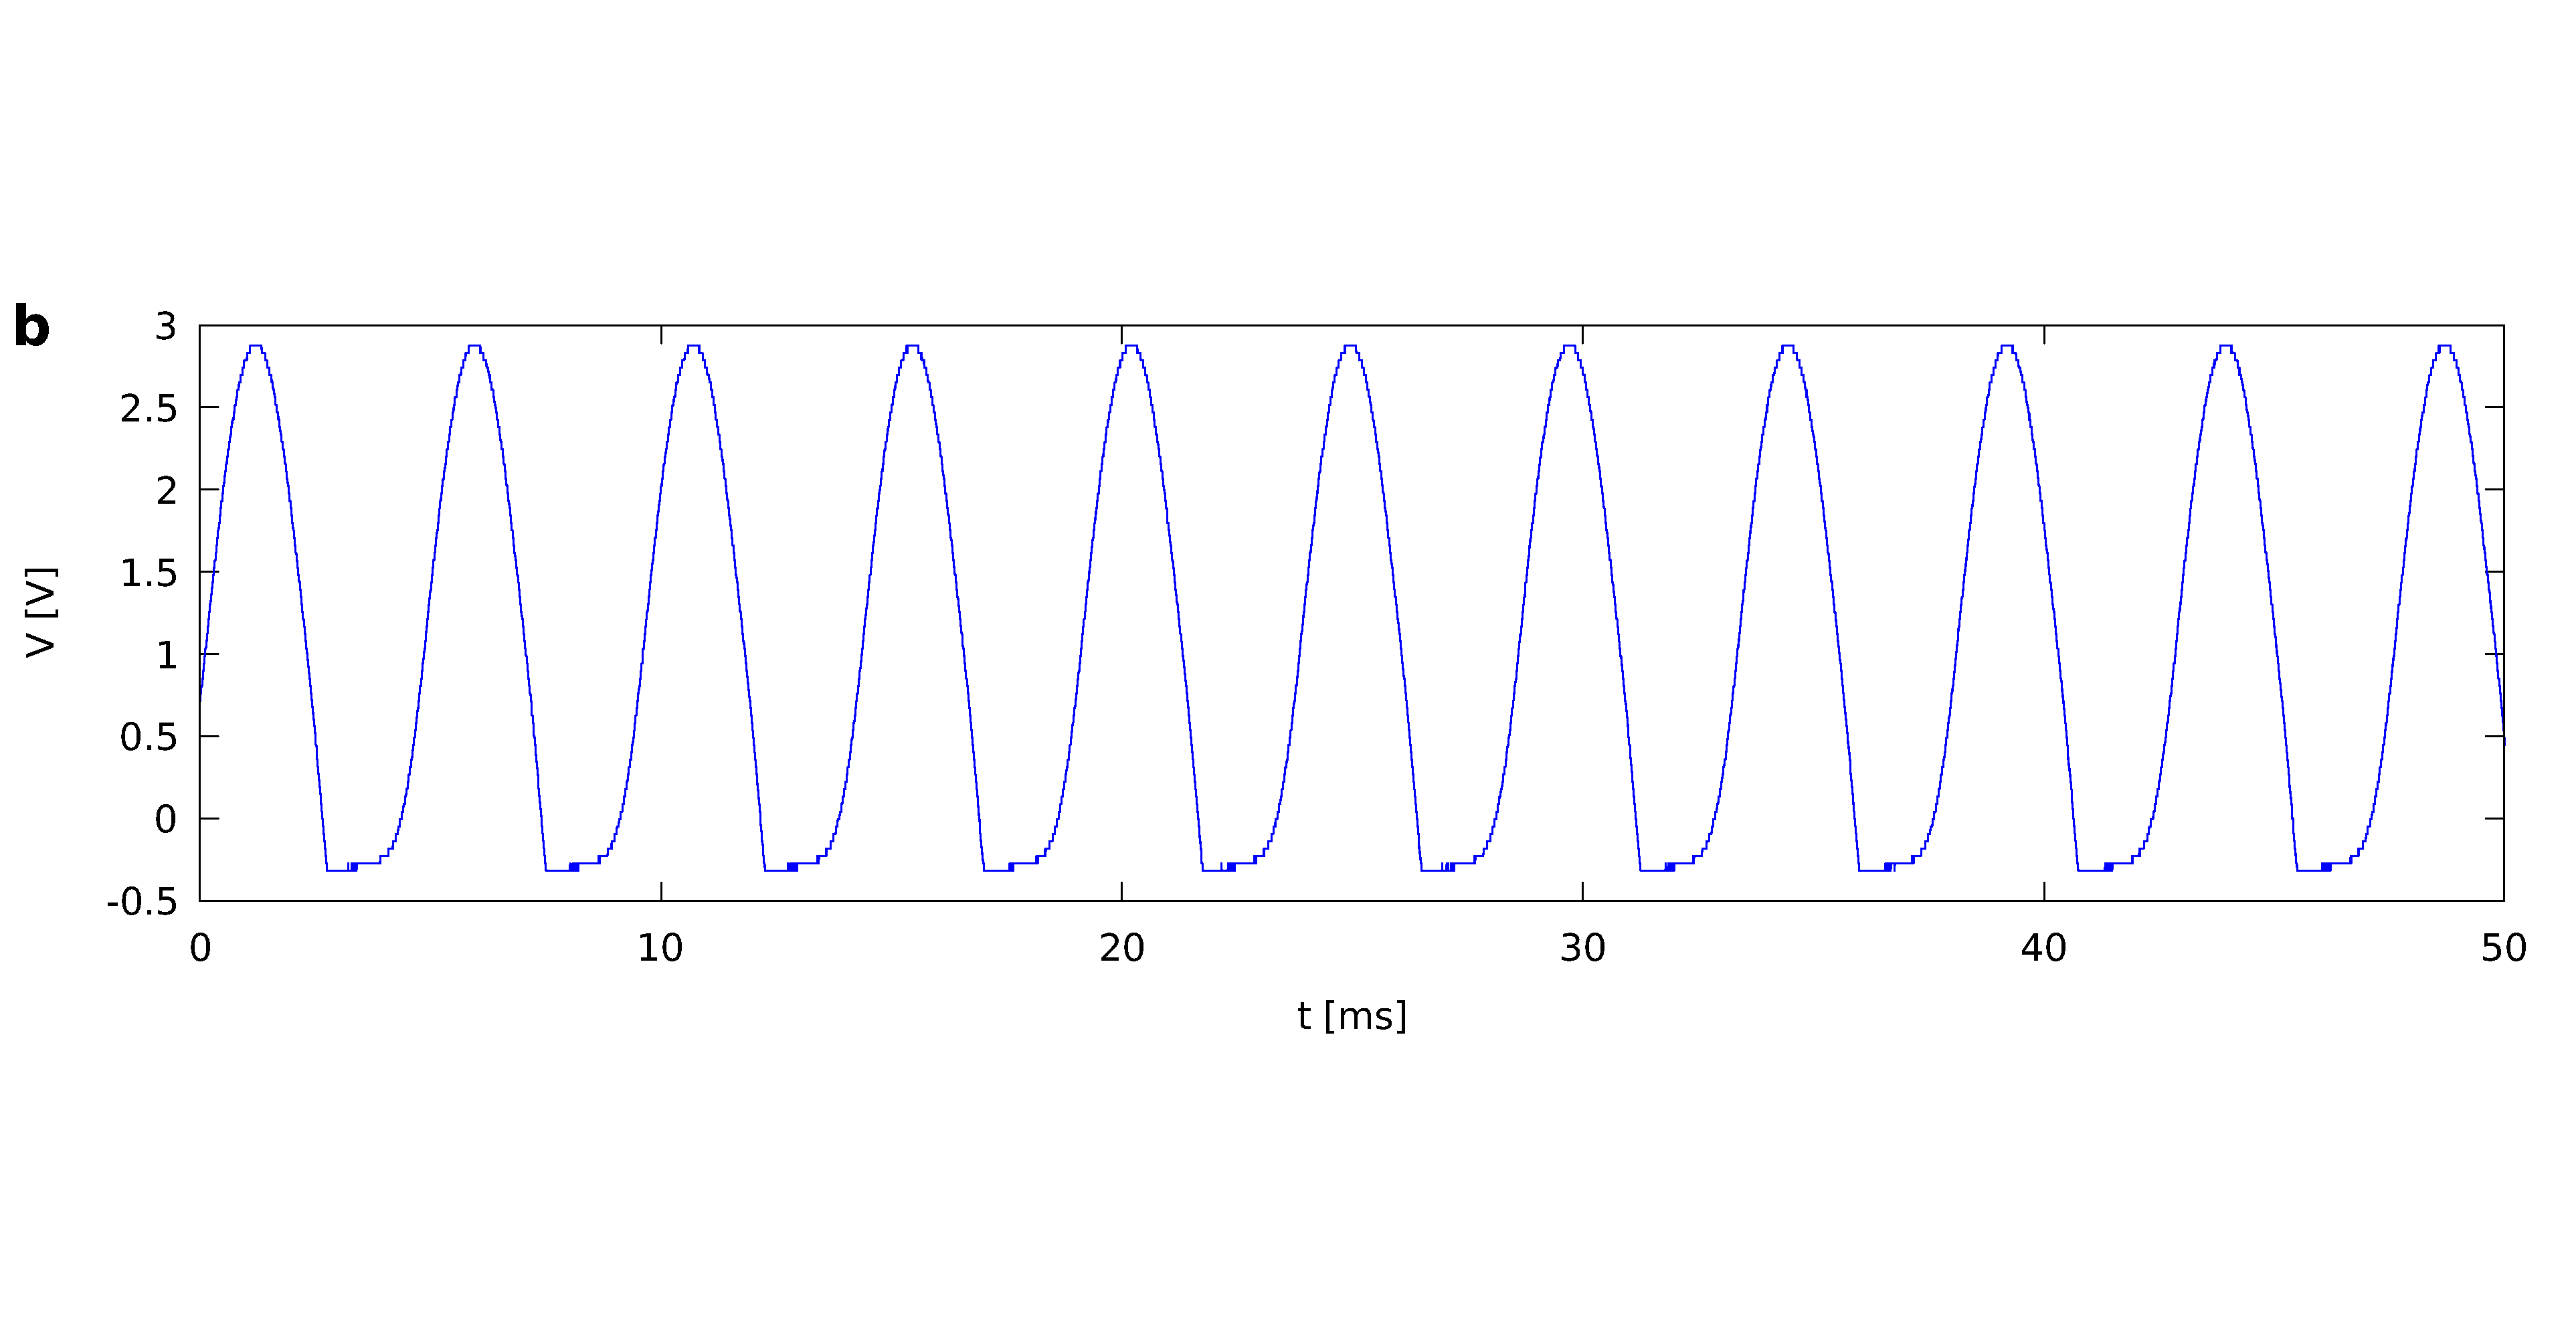
\includegraphics[width=\linewidth,trim={0 6cm 0 6cm},clip,left]
            {../1_block/board_new/V_wf.pdf}
        \end{subfigure}
    \end{minipage}
    \begin{subfigure}{.39\textwidth}
        \centering
        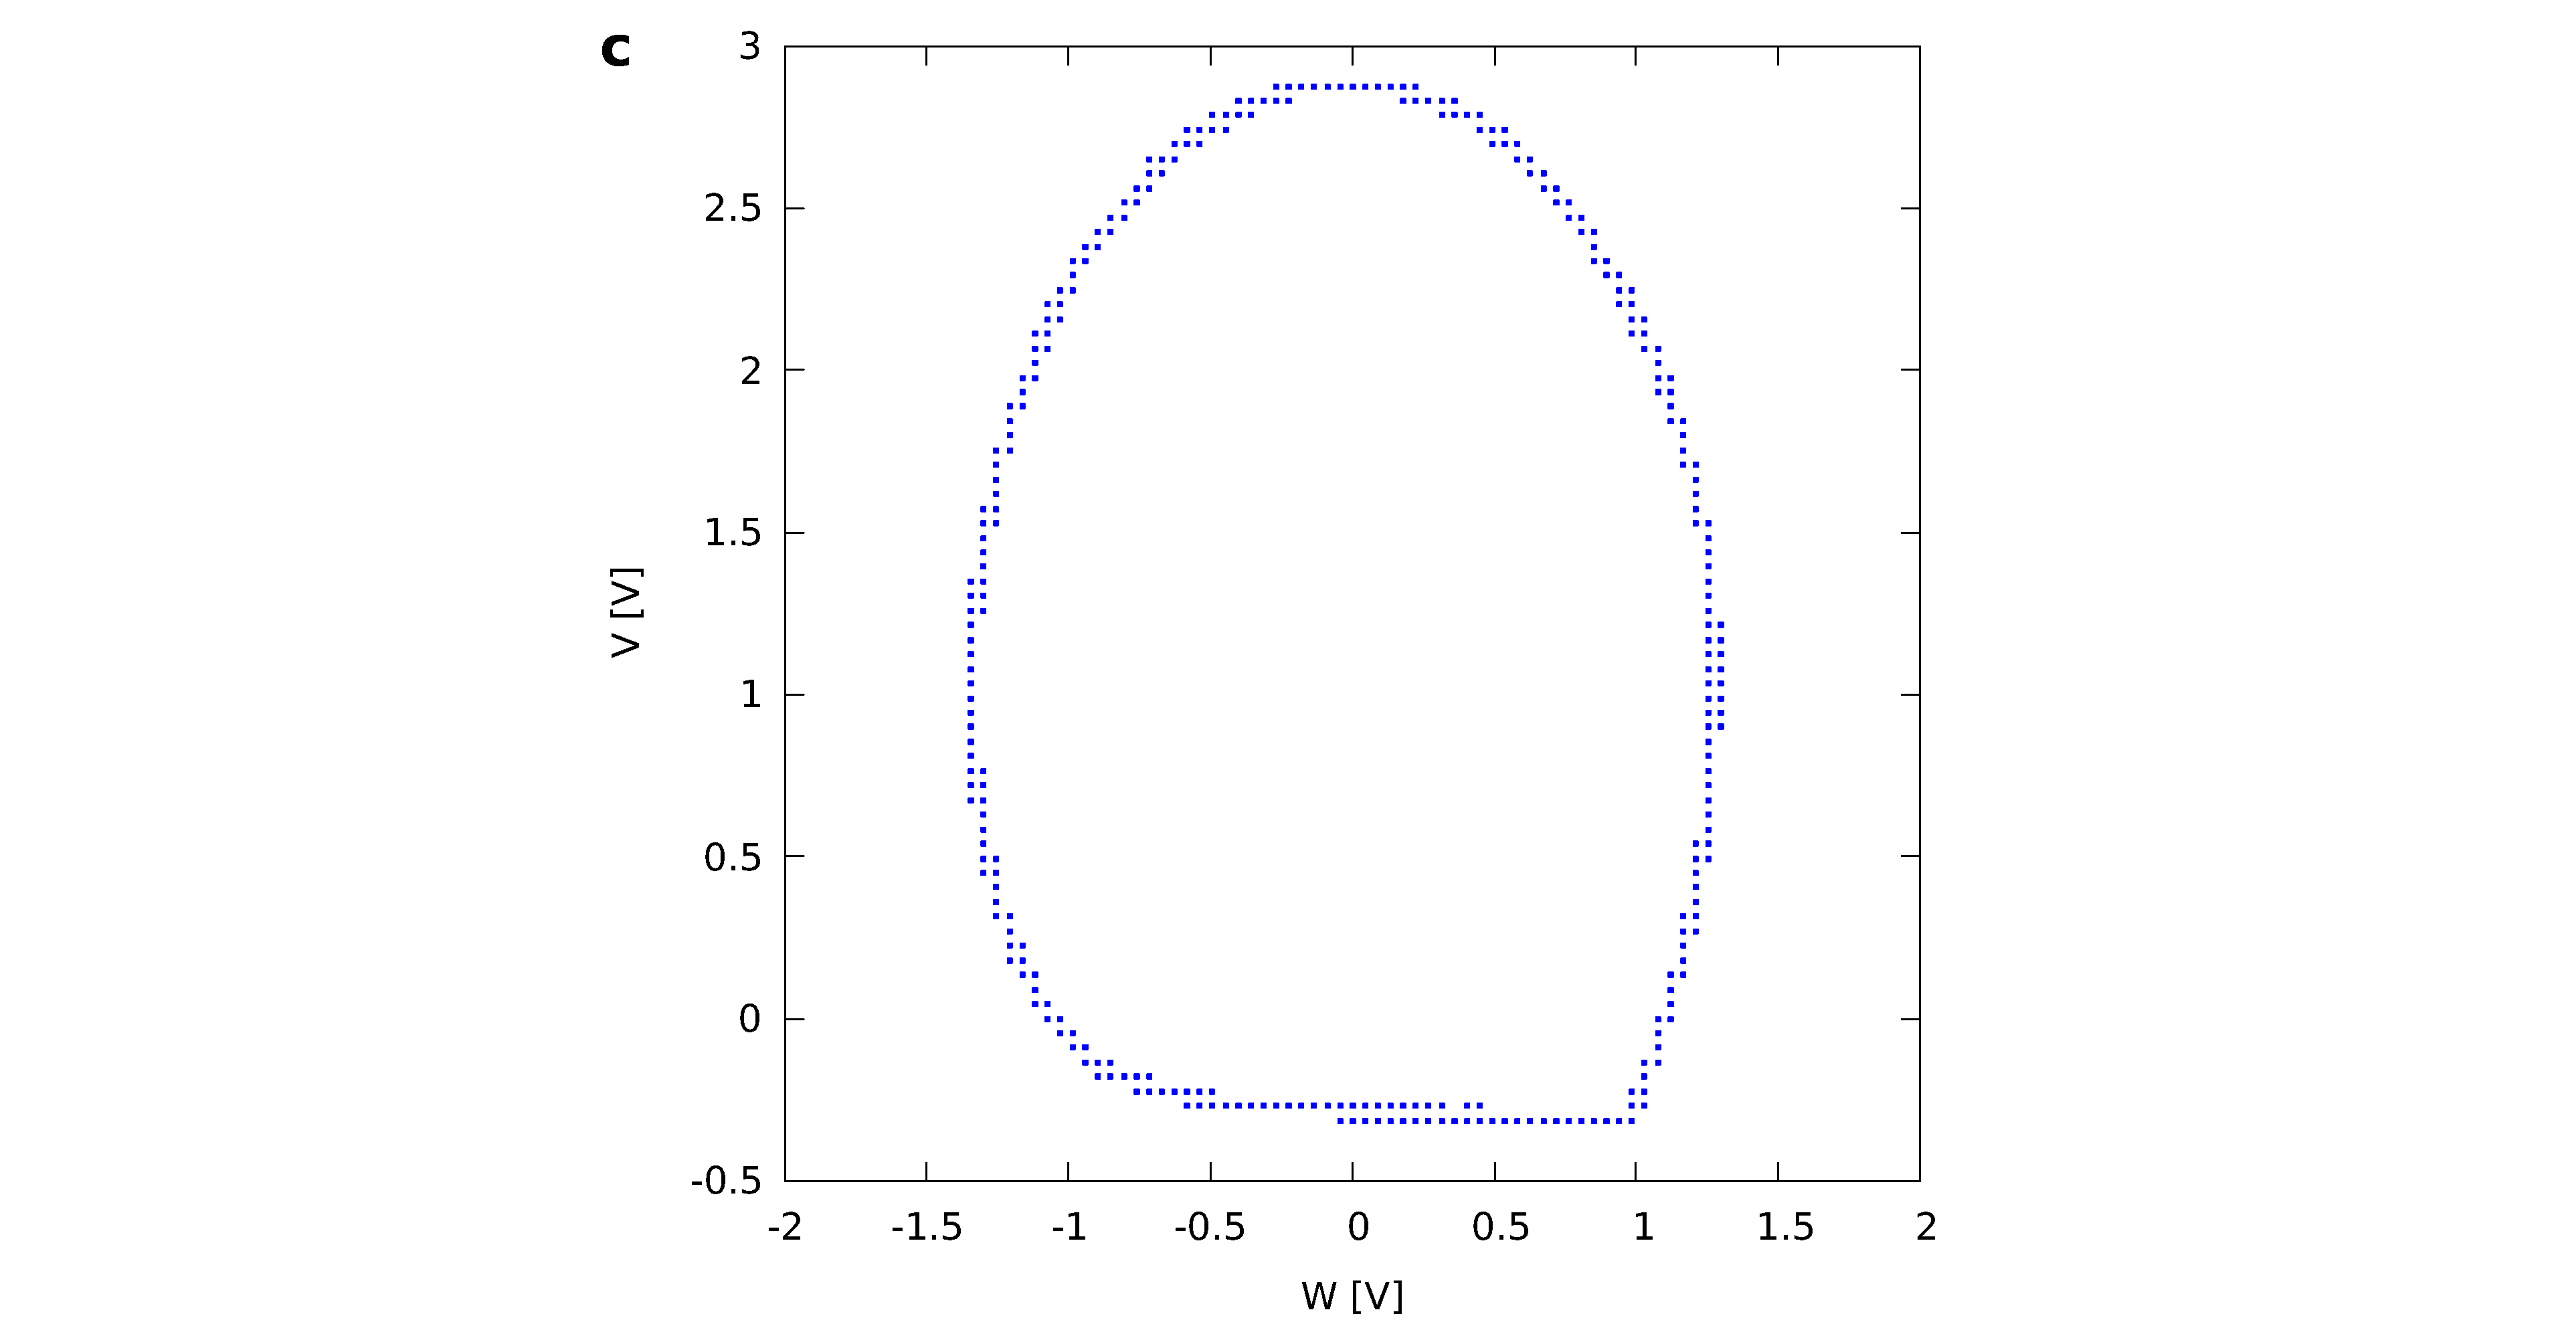
\includegraphics[width=\linewidth,trim={15cm 0 15cm 0},clip,right]
        {../1_block/board_new/Lissajous.pdf}
    \end{subfigure}
    \begin{subfigure}{.49\textwidth}
        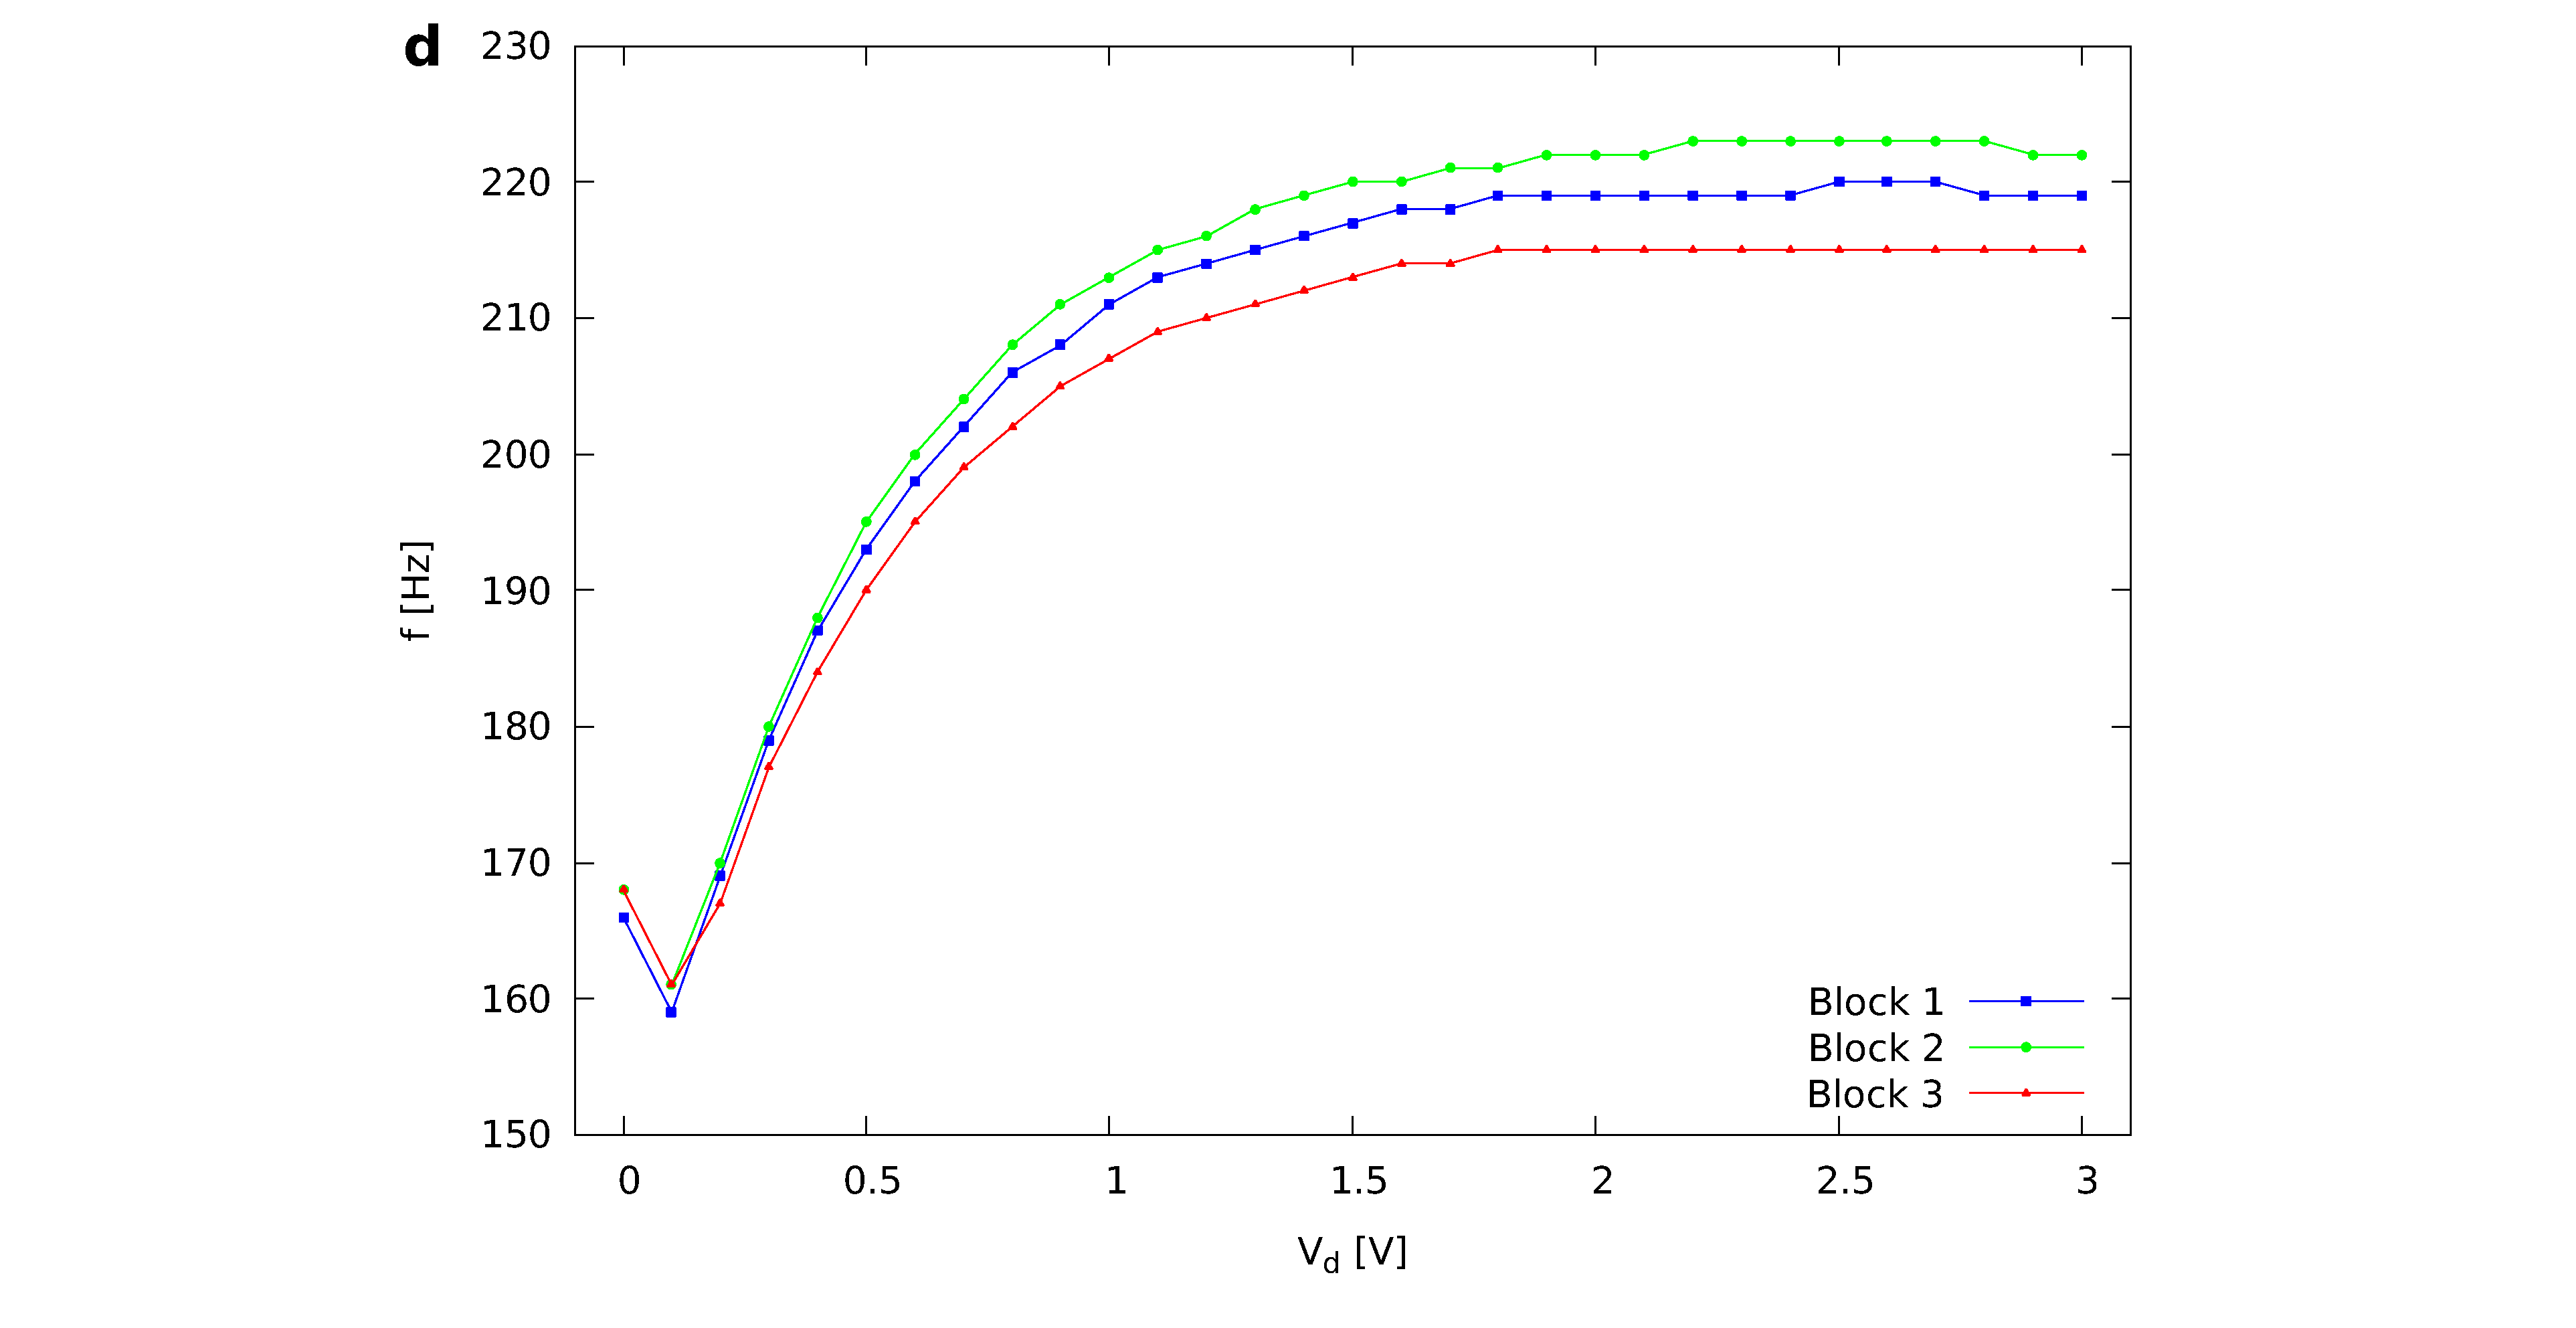
\includegraphics[width=\linewidth,trim={10cm 0 9cm 0},clip,left]
        {../1_block/board_new/freq_board.pdf}
    \end{subfigure}
    \begin{subfigure}{.49\textwidth}
        \centering
        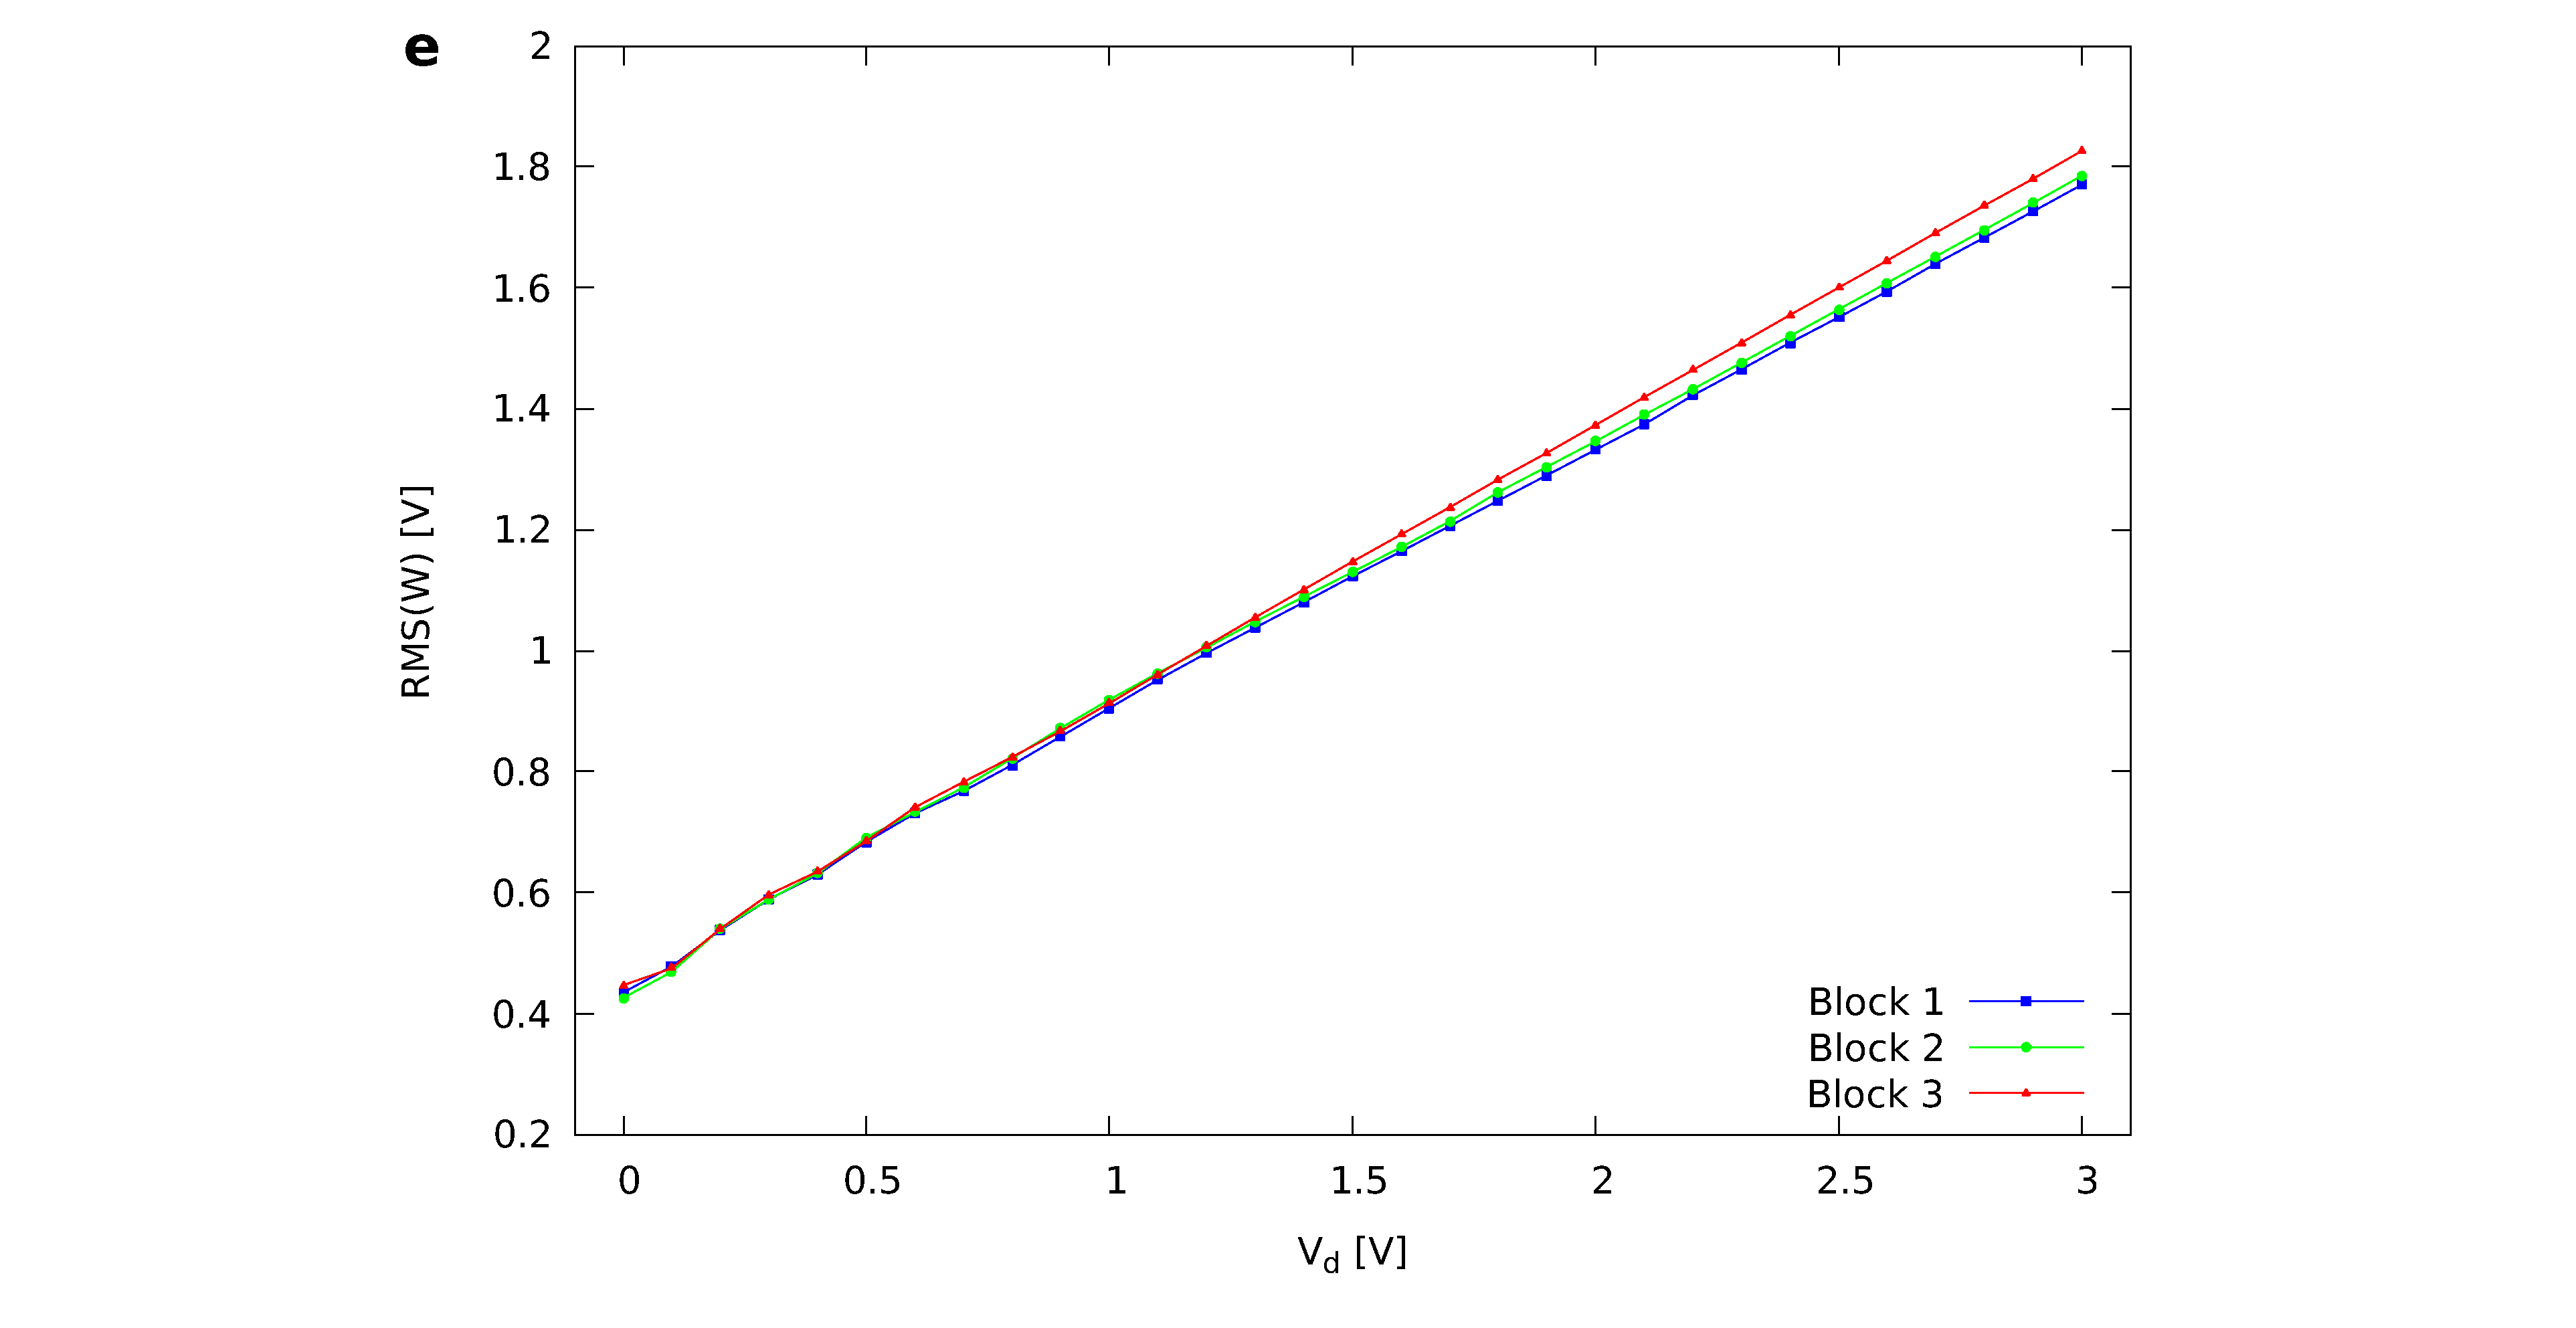
\includegraphics[width=\linewidth,trim={9cm 0 10cm 0},clip,right]
        {../1_block/board_new/rms_board.pdf}
    \end{subfigure}
    \caption{Oscillating behavior for the circuit implemented on
    the new board. (a) Plot of $W$ and (b) of $V$ as a
    function of time, for $V_d=1$ V.
    (c) Phase portrait (Lissajous figure) of $V$ versus $W$. (d)
    Frequency and (e) root mean square amplitude of the
    output signal $W$ as a function of the parameter $V_d$ and for
    three different blocks.}
    \label{fig:oscillation board new}
\end{figure}

\section{Conclusions}\label{sec:conclusions}

The comparison between frequency and amplitude on the three
implementations is shown in Fig. \ref{fig:comparison}.
The frequency of the board is very similar to the breadboard one
for voltages $V_d < 1$ V; at higher voltages there are small
deviations in the board, probably due to the increased relevance
of the current clamping. This might also be the reason why the
amplitude behavior of the board is not linear.

\begin{figure}[H]
    \centering
    \begin{subfigure}{.49\textwidth}
        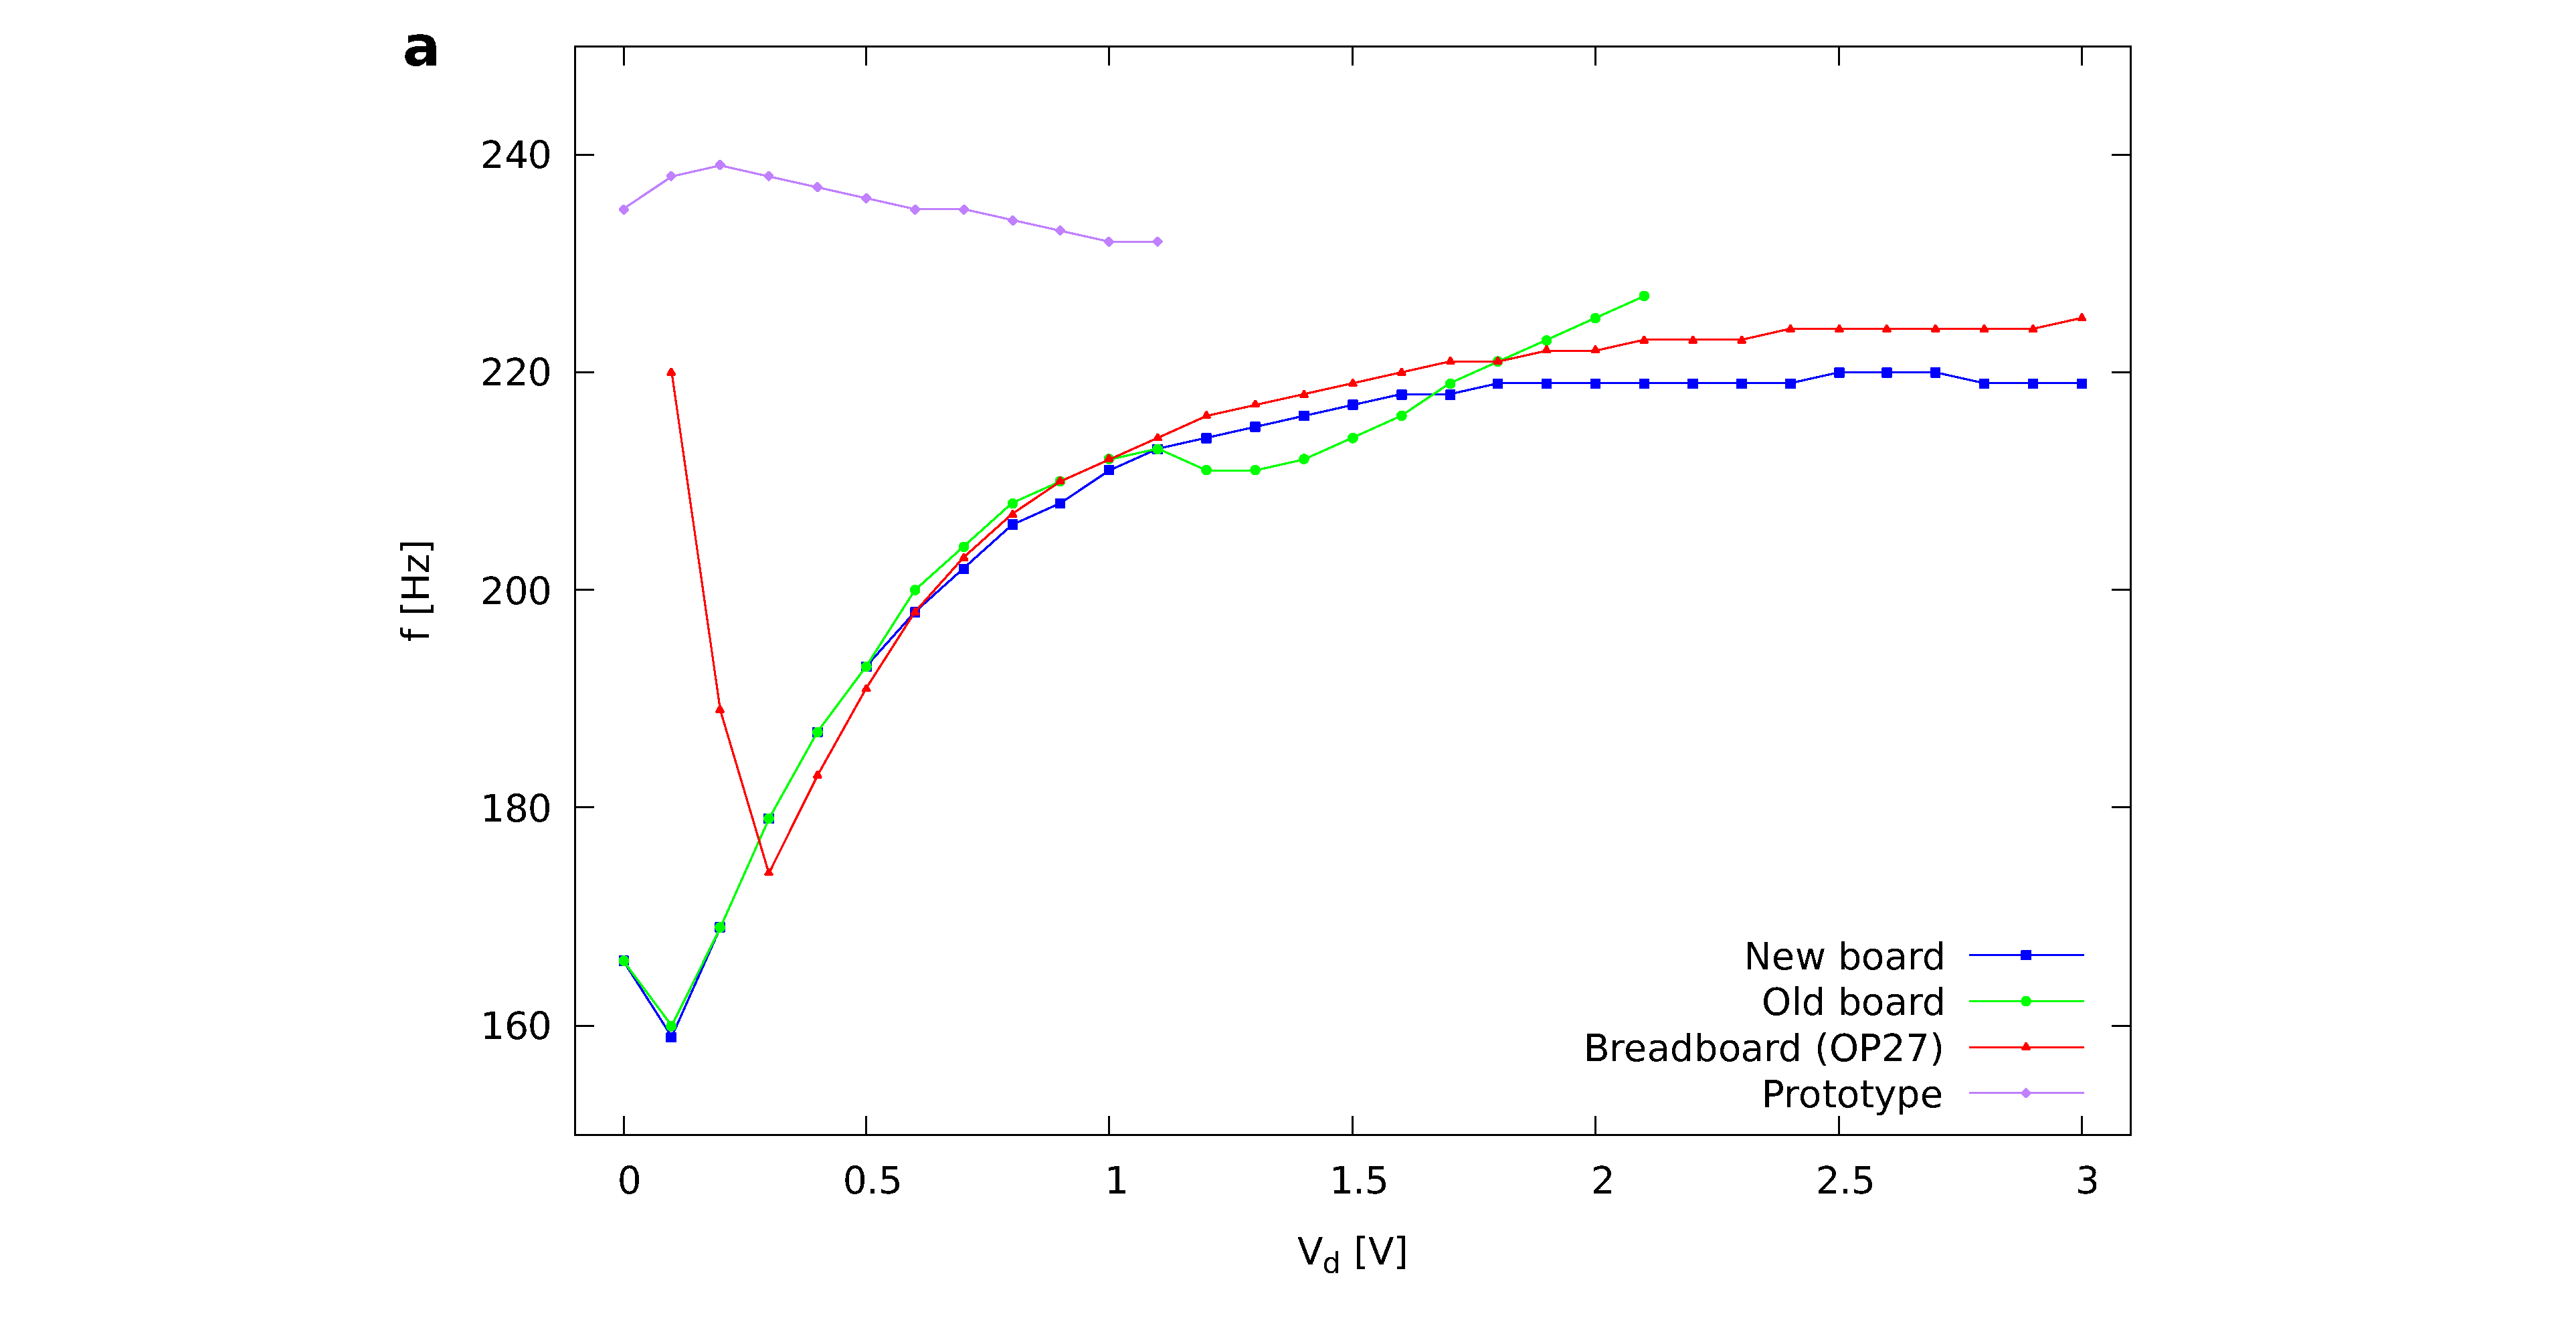
\includegraphics[width=\linewidth,trim={10cm 0 9cm 0},clip,left]
        {../1_block/images/freq_comparison.pdf}
    \end{subfigure}
    \begin{subfigure}{.49\textwidth}
        \centering
        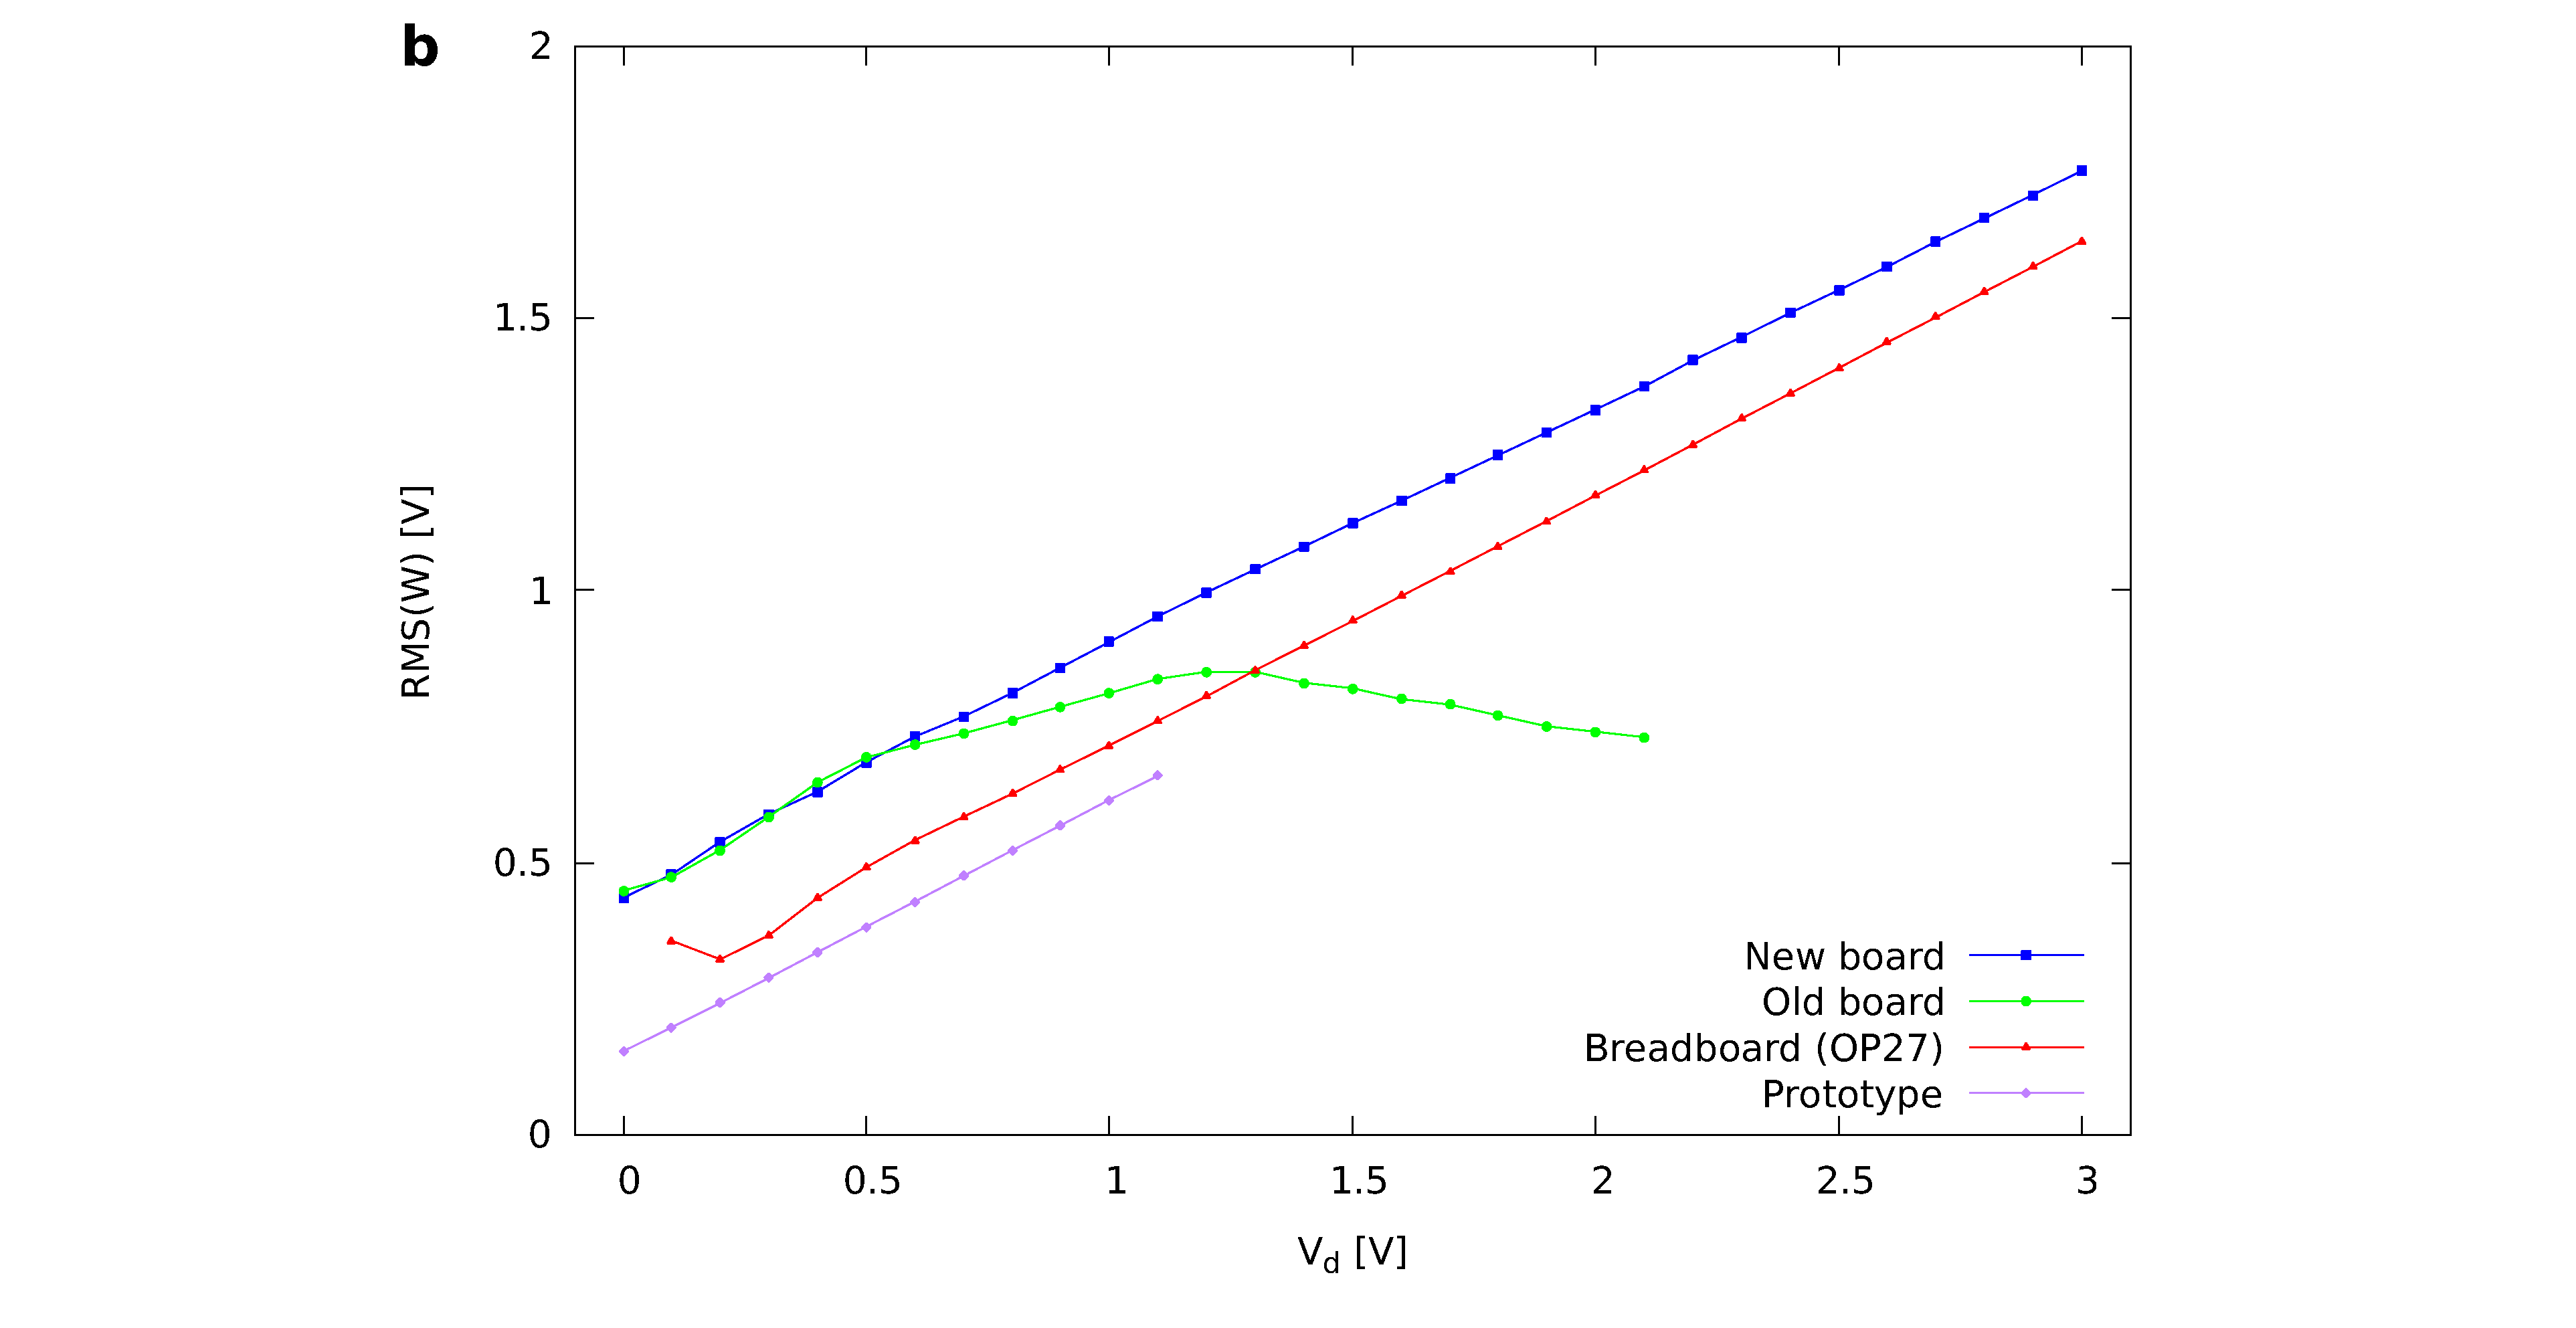
\includegraphics[width=\linewidth,trim={9cm 0 10cm 0},clip,right]
        {../1_block/images/rms_comparison.pdf}
    \end{subfigure}
    \caption{(a) Frequency and (b) root mean square amplitude
    of the output signal $W$ as a function of the parameter $V_d$
    for the three implementations of the BK model, i.e. the first
    block of the board, the breadboard implementation with the
    OP27 op-amps and the first prototypical chip.}
    \label{fig:comparison}
\end{figure}

\end{comment}